\documentclass[12pt]{article}
\usepackage[T1]{fontenc}
\usepackage[utf8]{inputenc}
\usepackage[polish]{babel}
\usepackage{graphicx}
\usepackage{geometry}
\usepackage{hyperref}
\usepackage{longtable}
\usepackage{booktabs}
\usepackage{float}
\usepackage{fancyhdr}

\renewcommand{\normalsize}{\fontsize{9}{11}\selectfont}
\normalsize

\geometry{a4paper, margin=2.5cm}
\title{{\Huge Analiza F1} \\ \small Dokumentacja Projektu Hurtowni Danych}
\author{Hubert Sobociński i Paweł Pozorski \\ \small Politechnika Warszawska, Wydział Matematyki i Nauk Informacyjnych}
\date{\today}

\pagestyle{fancy}
\fancyhf{}
\fancyhead[L]{Sobociński \& Pozorski}
\fancyhead[R]{Analiza F1}
\fancyfoot[C]{\thepage}
\renewcommand{\headrulewidth}{0.4pt}
\renewcommand{\footrulewidth}{0pt}

\begin{document}

\maketitle

\begin{abstract}
    Celem projektu jest stworzenie kompleksowej hurtowni danych dedykowanej zespołom Formuły 1, umożliwiającej integrację, analizę oraz raportowanie danych wyścigowych z różnych sezonów. System będzie wspierał strategiczne decyzje konstruktorów, kierowców i analityków, zapewniając spójne i wysokiej jakości informacje o wynikach, postępach oraz statystykach. Planowana architektura rozwiązania opiera się na centralnym repozytorium danych, które pozwoli na łatwy dostęp, porównywanie sezonów oraz generowanie prognoz. Projekt przyniesie korzyści zarówno decydentom, jak i kibicom, zwiększając zaangażowanie i jakość analiz w świecie F1.
\end{abstract}

\newpage
\tableofcontents
\newpage

\section{Cel projektu i planowane korzyści}
Celem projektu jest stworzenie hurtowni danych dla zespołów F1, która będzie gromadziła i analizowała informacje dotyczące konstruktorów, ich wyników oraz osiągnięć w poszczególnych sezonach wyścigowych. Hurtownia danych ma na celu integrację danych z różnych źródeł w jednym centralnym repozytorium, co umożliwi zaawansowaną analizę i generowanie raportów na temat wyników wyścigów, pozycji w mistrzostwach, oraz statystyk związanych z konkretnymi konstruktorami.

Główne cele projektu to:

\begin{itemize}
    \item Zgromadzenie różnych szczegółowych danych na temat wyścigów F1.
    \item Umożliwienie łatwego dostępu do danych z różnych lat, co pozwoli na porównanie wyników konstruktorów oraz kierowców w danym sezonie oraz na przestrzeni lat.
    \item Tworzenie raportów dotyczących postępów konstruktorów czy kierowców, które będą użyteczne zarówno dla menedżerów wyścigów, jak i analityków sportowych.
    \item Zapewnienie wysokiej jakości danych, które będą zgodne z wymaganiami raportowania w branży wyścigowej.
\end{itemize}

\subsection{Planowane korzyści z perspektywy odbiorcy rozwiązania}

Hurtownia danych umożliwi właścicielom drużyn, konstruktorom, kierowcą czy kibicom dostęp do istotnych informacji, co pozwoli im na podejmowanie lepszych decyzji strategicznych, a dla kibiców na przykład wybór ciekawszych wyścigów do oglądania. Główne korzyści dla użytkowników końcowych to:

\begin{itemize}
    \item \textbf{Lepsza analiza wyników wyścigów:} Hurtownia danych pozwoli na szybkie i dokładne analizowanie wyników poszczególnych wyścigów, co umożliwi ocenę efektywności konstruktorów w danym sezonie oraz porównanie ich wyników na przestrzeni lat.
    \item \textbf{Łatwiejsze raportowanie:} Zintegrowane dane w jednej hurtowni umożliwią szybkie generowanie raportów na potrzeby władz sportowych, sponsorów czy mediów, co usprawni procesy raportowe w wyścigach.
    \item \textbf{Lepsze prognozy:} Dzięki obszernym danym dotyczącym wyników i pozycji w mistrzostwach, możliwe będzie opracowanie bardziej trafnych prognoz dotyczących przyszłych wyników, które będą użyteczne zarówno dla analityków, jak i dla sponsorów czy mediów.
    \item \textbf{Lepsza organizacja i informacja dla kibiców:} Centralizacja danych pozwoli także na przygotowanie uporządkowanego terminarza wyścigów oraz łatwy dostęp do szczegółowych informacji o torach, co zwiększy zaangażowanie i satysfakcję kibiców.
\end{itemize}


Dzięki tym korzyściom, hurtownia danych przyczyni się do wzrostu efektywności zarządzania zespołami wyścigowymi, a także umożliwi lepsze podejmowanie decyzji opartych na danych. W dłuższej perspektywie projekt przyczyni się do poprawy konkurencyjności w wyścigach, dzięki dostarczeniu zespołom i analitykom narzędzi do lepszego zarządzania i analizy danych.
\section{Diagram i Opis Architektury Rozwiązania}
W ramach projektu zaplanowano następującą architekturę rozwiązania:

\begin{itemize}
    \item Prefect jako narzędzie do organizacji procesów ETL,
    \item Zbiory danych w formacie CSV,
    \item Hurtownia danych oparta na bazie SQL, w której przechowywane będą wyniki wyścigów, dane o torach, uczestnikach i inne,
    \item Raportowanie z wykorzystaniem narzędzi Business Intelligence.
\end{itemize}

\begin{figure}[h!]
    \centering
    \includegraphics[width=0.95\textwidth]{Mapa myśli (2).png}
    \caption{Diagram architektury rozwiązania}
\end{figure}

\subsection{Opis architektury}

\begin{itemize}
    \item \textbf{Prefect Cloud:} Początkowo aplikacja była hostowana na
    \href{https://app.prefect.cloud}{chmurze Prefect}, co umożliwiało centralne zarządzanie procesami ETL. Niestety, w darmowej wersji Prefect Cloud nie było wsparcia dla połączeń z bazą danych MSSQL, dlatego zdecydowaliśmy się na uruchomienie systemu lokalnie.
    \item \textbf{Azure MSSQL:} Baza danych MSSQL jest hostowana na platformie Azure
    \\(\texttt{hurtownie.database.windows.net}), co zapewnia wysoką dostępność i bezpieczeństwo danych. (Ze względu na ograniczone możliwości korzystania z platformy Azure to znaczy wykorzystanie darmowych zasobów, postawiliśmy później hurtownie lokalnie)
    \item \textbf{Lokalne hostowanie:} Testowo aplikacja działa z wykorzystaniem lokalnych zasobów i pełnej kontroli nad połączeniami do baz danych. System wciąż automatycznie pobiera najnowszy kod z repozytorium GitHub, co ułatwia rozwój i aktualizację aplikacji bez potrzeby jej resetowania.

\end{itemize}

\subsection{Bezpieczeństwo połączenia z bazą danych}

Dostęp do bazy MSSQL jest bezpieczny dzięki wdrożeniu kilku mechanizmów ochrony:
\begin{itemize}
    \item \textbf{Firewall z whitelistą IP:} Aby zapewnić, że tylko autoryzowane adresy IP mogą uzyskać dostęp do bazy danych, skonfigurowano firewall z whitelistą dozwolonych adresów IP.
    \item \textbf{Logowanie po SQL:} Użytkownicy mogą logować się do bazy danych za pomocą standardowego logowania SQL, co zapewnia bezpieczeństwo dostępu oraz audyt działań użytkowników.
    \item \textbf{MS Authenticator:} Dodatkowo, osoby, które mają mieć dostęp do bazy danych przez narzędzia i muszą wykonywać operacje bezpośrednio na bazie danych, są zmuszone do korzystania z aplikacji MS Authenticator, co umożliwia uwierzytelnienie dwuetapowe i zwiększa bezpieczeństwo dostępu.
\end{itemize}

\section{Wykorzystywane zbiory danych}

Projekt wykorzystuje trzy główne źródła danych:

\begin{table}[ht]
\centering
\begin{tabular}{|p{4cm}|p{5cm}|p{2.5cm}|p{3cm}|}
\hline
\textbf{Zbiór danych} & \textbf{Źródło} & \textbf{Format danych} & \textbf{Częstotliwość odświeżania} \\
\hline
Dane historyczne F1 (kierowcy, zespoły, wyścigi, wyniki, itd.) & \href{https://github.com/f1db/f1db}{f1db GitHub} – zestaw plików CSV z pełną bazą danych F1 & CSV & Co tydzień po wyścigu \\
\hline
Frekwencje na Grand Prix & Zescrapowane dane ze strony: \href{https://f1destinations.com/resources/f1-attendance-figures/}{f1destinations.com} & Ręcznie stworzona CSV & Co tydzień po wyścigu\\
\hline
Dane o torach wyścigowych (lokalizacja, długość, typ, itp.) & Zescrapowane ze strony: \href{https://www.racingcircuits.info}{racingcircuits.info} & Ręcznie stworzona CSV & Co miesiąc\\
\hline
\end{tabular}
\caption{Wykorzystywane zbiory danych}
\end{table}

Dane z repozytorium \texttt{f1db} obejmują m.in. tabele: \texttt{drivers.csv}, \texttt{constructors.csv}, \texttt{races.csv}, \texttt{results.csv}, \texttt{circuits.csv} i inne, które razem tworzą pełną relacyjną bazę danych Formuły 1.

Zescrapowane dane z dwóch stron internetowych uzupełniają brakujące informacje niedostępne w \texttt{f1db}, takie jak liczba widzów na torze oraz szczegółowe parametry torów.

\section{Proces ETL}

\textbf{ETL} to proces służący do ekstrakcji danych, ich transformacji oraz załadowania do systemu docelowego. Nasz proces ETL wykorzystuje Prefect do zarządzania i harmonogramowania zadań, które realizują poszczególne etapy tego procesu.

\subsection{Extract}

Dane są ekstraktowane z różnych źródeł, w tym:
\begin{itemize}
    \item Z repozytorium GitHub, gdzie znajduje się kod aplikacji.
    \item Z baz danych MSSQL, z których pobierane są dane wymagające przetworzenia.
    \item Z zewnętrznych źródeł CSV.
\end{itemize}

\subsection{Transform}

Proces transformacji obejmuje następujące kroki:
\begin{itemize}
    \item \textbf{Czyszczenie danych:} Usuwanie nieprawidłowych rekordów, uzupełnianie brakujących danych.
    \item \textbf{Zmiana struktury danych:} Normalizacja danych.
    \item \textbf{Walidacja danych:} Sprawdzanie poprawności danych.
    \item \textbf{Agregacja danych:} Grupowanie danych w celu uzyskania bardziej skondensowanej i użytecznej formy.
\end{itemize}

W ramach procesu ETL (Extract, Transform, Load) dokonaliśmy szeregu przekształceń danych, które umożliwiają uzyskanie wymaganych wyników w strukturze analitycznej. Poniżej przedstawiono szczegółowy opis poszczególnych kroków transformacji danych.


\begin{enumerate}
    \item \textbf{Season\_tyre\_manufacturer → usunięte}

    \textbf{Opis:} Sezonowe wyniki producenta opon (Season\_tyre\_manufacturer) da się wyliczyć za pomocą \texttt{Fact\_Race\_Data}

    \item \textbf{Season\_constructor + constructor →usunięte}

    \textbf{Opis:} Sezonowe wyniki konstruktora (Season\_constructor) da się wyliczyć za pomocą \texttt{Fact\_Race\_Data}


    \item \textbf{Season\_engine\_manufacturer → usunięte}

    \textbf{Opis:} Sezonowe wyniki producenta silników (Season\_engine\_manufacturer) da się wyliczyć za pomocą \texttt{Fact\_Race\_Data}

    \item \textbf{Season\_driver + Season\_driver\_standing → usunięte}

    \textbf{Opis:} Sezonowe wyniki kierowców (Season\_driver + Season\_driver\_standing) da się wyliczyć za pomocą \texttt{Fact\_Race\_Data}

    \item \textbf{Season\_entrant + entrant → entrant}

    \textbf{Opis:} Dane zespołów z sezonów oraz ogólne informacje o uczestnikach (entrant) zostały scalone w jedną tabelę \texttt{entrant}.

    \textbf{Agregacja:} Zapewnia pełne dane o zespołach i ich wynikach sezonowych.

    \item \textbf{Race + grand\_prix → Dim\_race}

    \textbf{Opis:} Połączenie danych o wyścigach (Race) oraz Grand Prix (grand\_prix) w tabeli \texttt{Dim\_race}. Dodano również nazwy krajów i nazwiska związane z Grand Prix.

    \textbf{Usunięcie:} Kolumna \texttt{total\_races\_held} została usunięta, ponieważ liczbę wyścigów można łatwo obliczyć przez agregację.

    \item \textbf{Country + continent → Dim\_country}

    \textbf{Opis:} Dane o kraju (Country) oraz kontynencie (continent) zostały połączone w tabeli \texttt{Dim\_country}, gdzie kontynent jest zawarty w danych o kraju.

    \item \textbf{Season\_entrant\_* – Usunięte}

    \textbf{Opis:} Kolumny \texttt{season\_entrant\_*} zostały usunięte, ponieważ dane te są już zawarte w tabeli \texttt{entrant}.

    \item \textbf{Season\_constructor\_standing → usunięto}

    \textbf{Opis:} Ranking konstruktorów da się uzyskać z tabeli \textit{Fact\_Race\_Data}

    \item \textbf{Chassis + engine + entrant → entrant}

    \textbf{Opis:} Informacje o podwoziu (\texttt{chassis}) i silniku (\texttt{engine}) połączono z tabelą \texttt{entrant}, uzupełniając ją o dane specyfikacyjne zespołów.


    \textbf{Opis:} Informacje o podwoziu (\texttt{chassis}) i silniku (\texttt{engine}) połączono z tabelą \texttt{entrant}, uzupełniając ją o dane specyfikacyjne zespołów.

\end{enumerate}

\subsection{Load}

Po przetworzeniu danych, są one ładowane do \textbf{Bazy MSSQL na Azure}


\section{Model fizyczny hurtowni danych}

Ze względu na rozbudowaną strukturę hurtowni danych oraz ograniczenia środowiska SQL Server Management Studio, nie było możliwe przejrzyste i estetyczne wyeksportowanie diagramu struktury bazy danych w formie graficznej.

W związku z tym, pełny model logiczny hurtowni został odtworzony w postaci skryptu SQL. Skrypt ten znajduje się w pliku \texttt{skrypt\_hurtowni\_danych.sql} i zawiera definicje wszystkich tabel, kluczy głównych oraz relacji między encjami.

\begin{figure}[H]
    \centering
    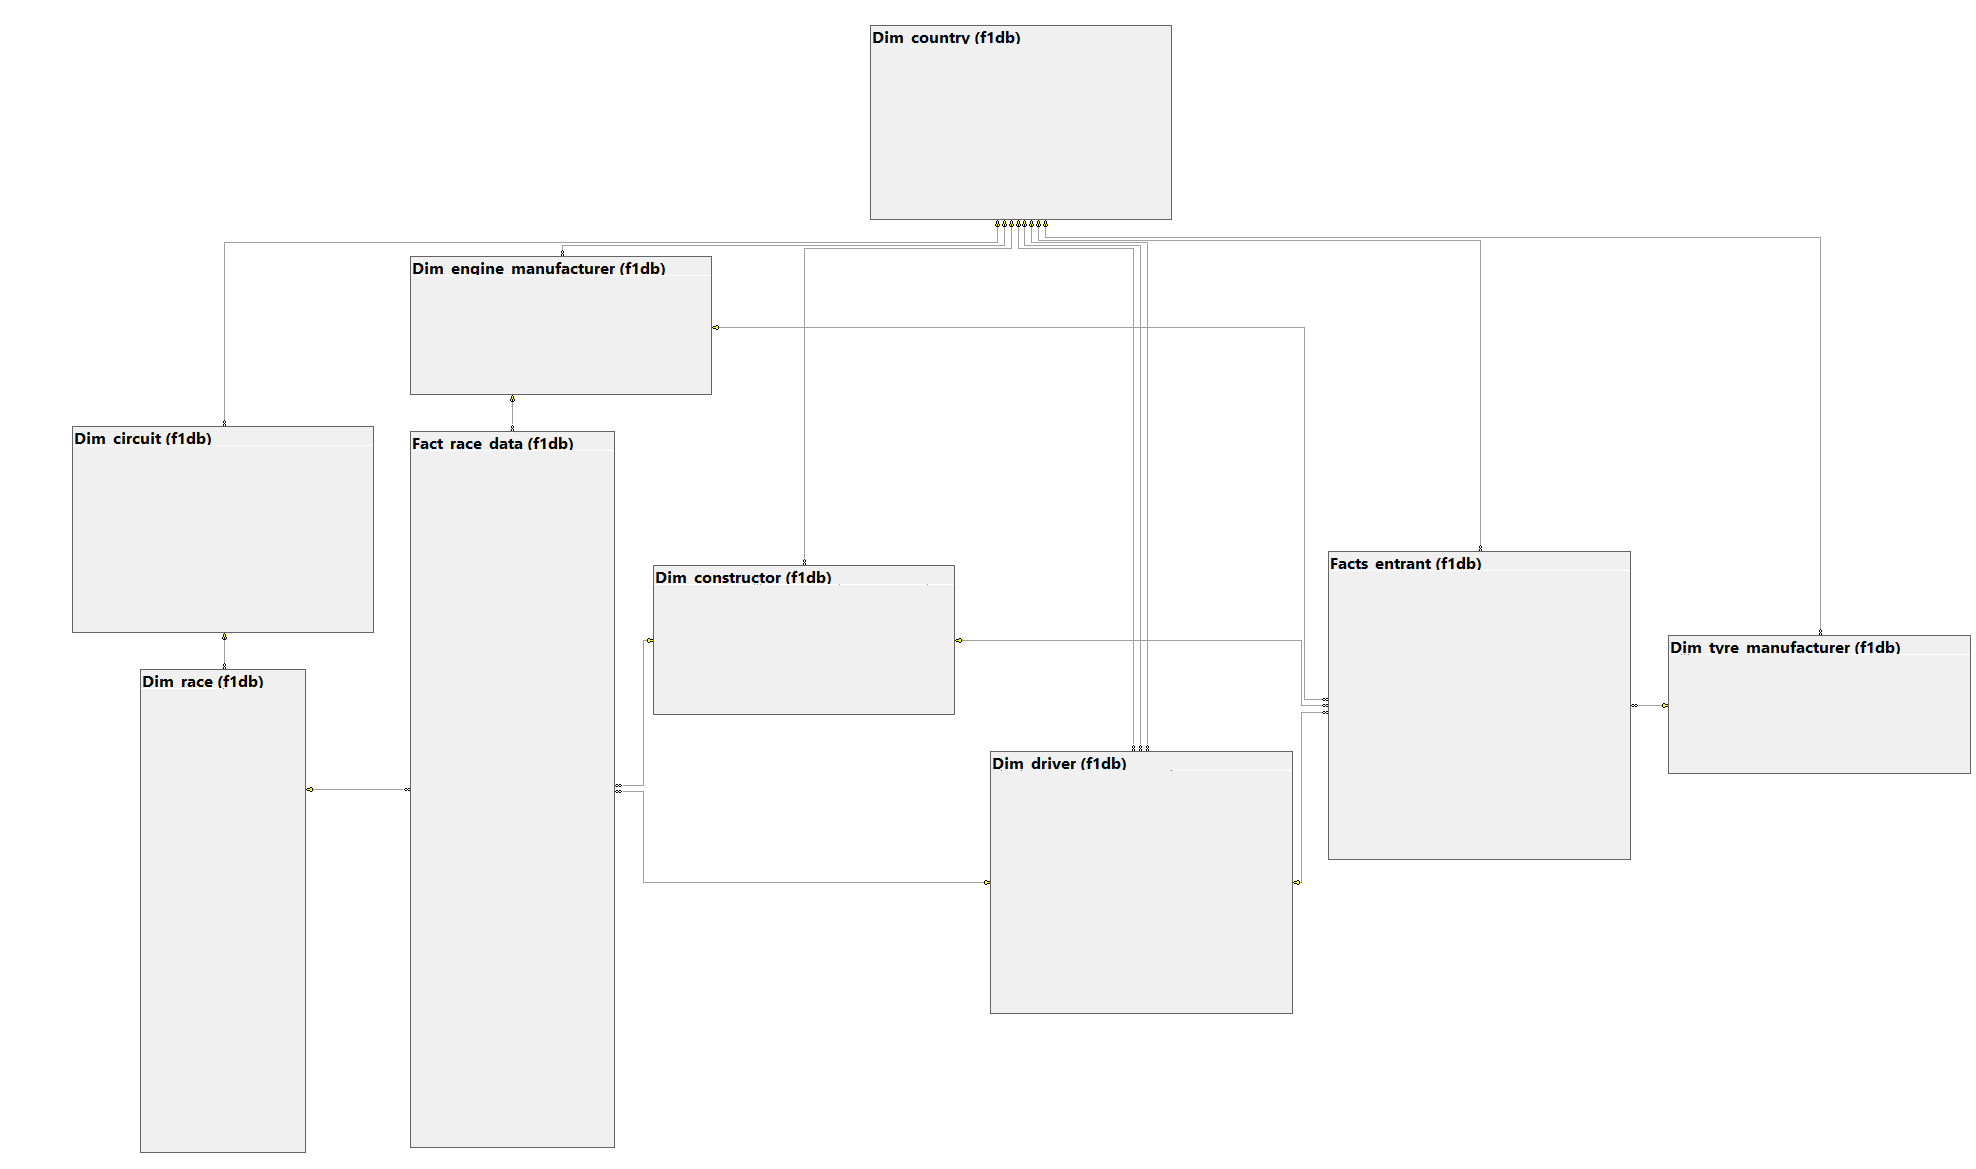
\includegraphics[width=\textwidth]{diagram1.png}
    \caption{Schemat hurtowni danych}
\end{figure}

\begin{figure}[H]
    \centering
    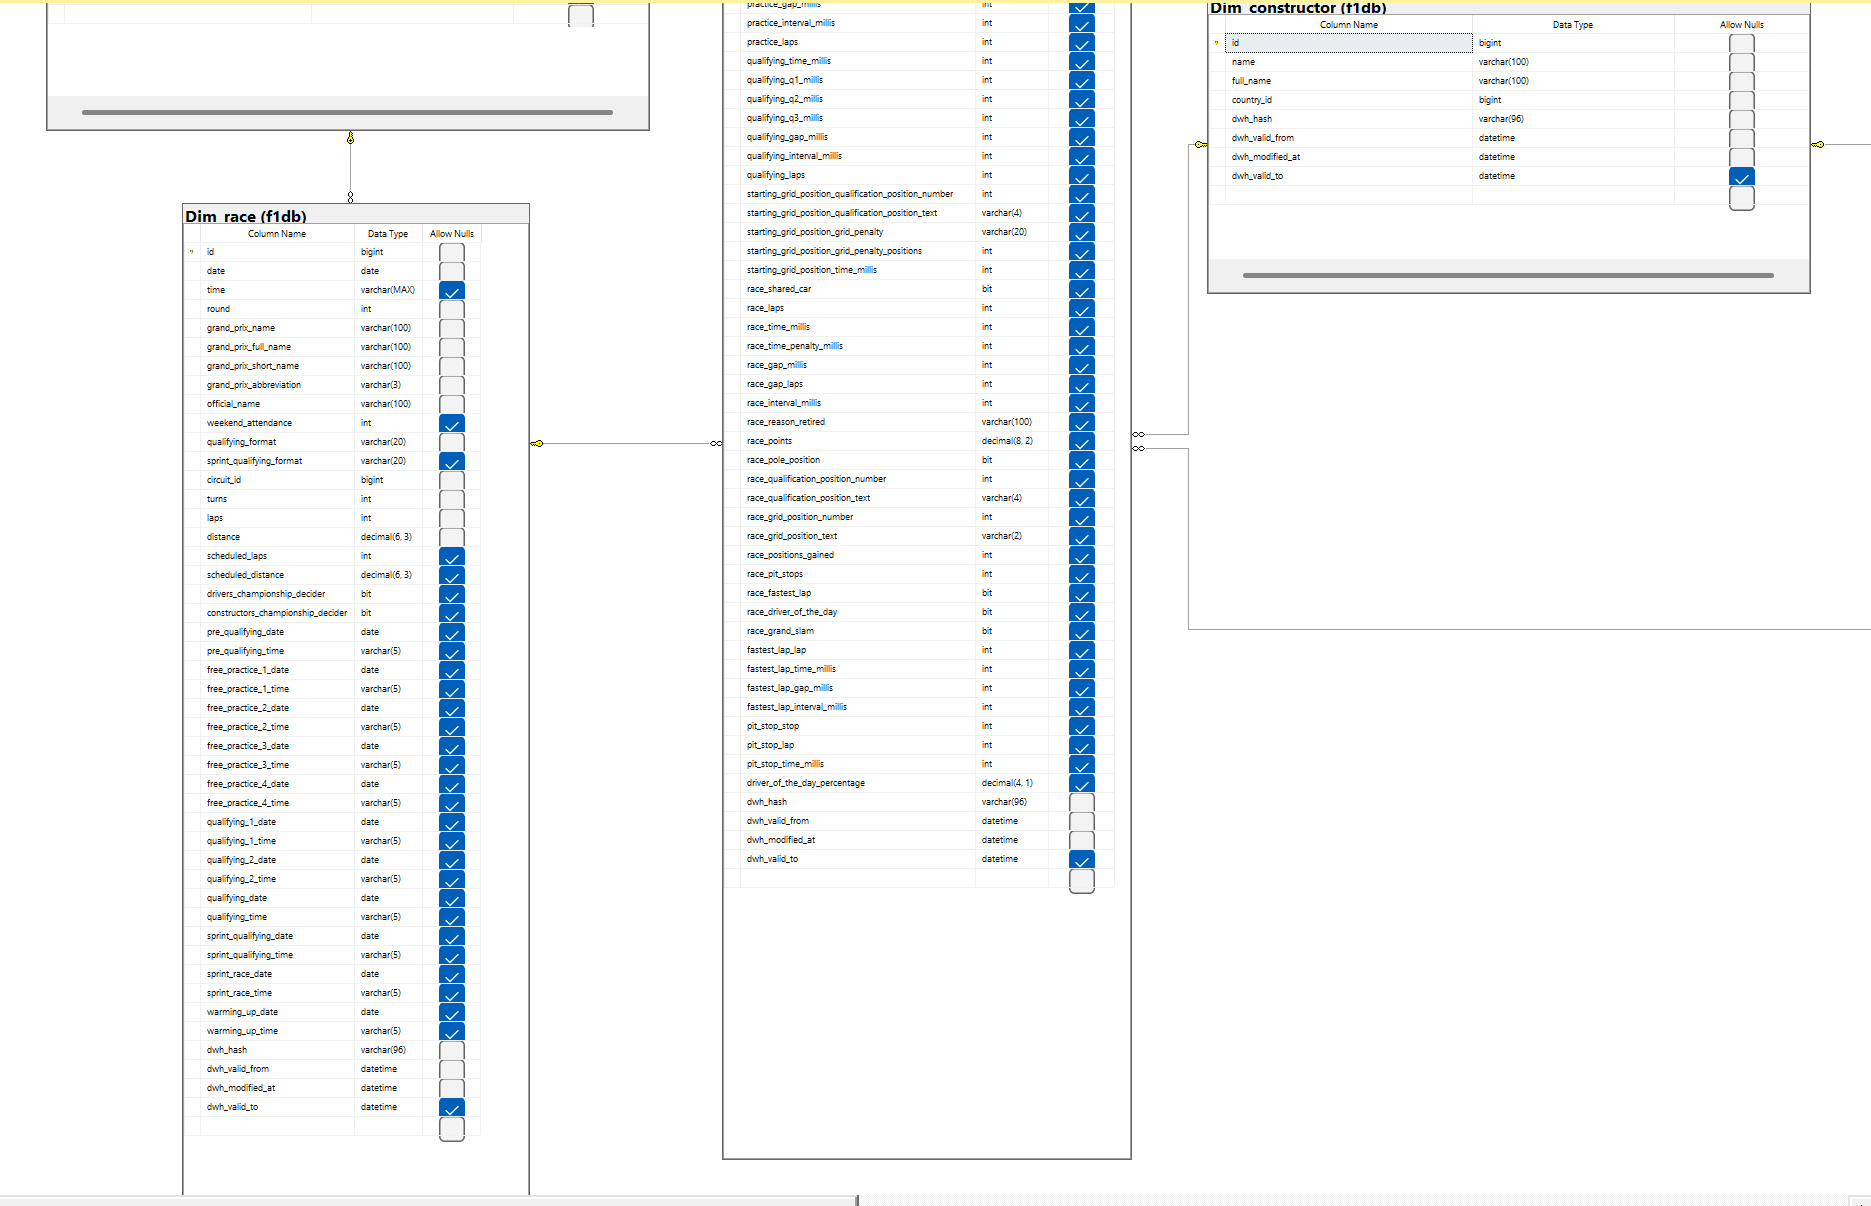
\includegraphics[width=\textwidth]{diagram2.png}
    \caption{Schemat hurtowni danych}
\end{figure}

\begin{figure}[H]
    \centering
    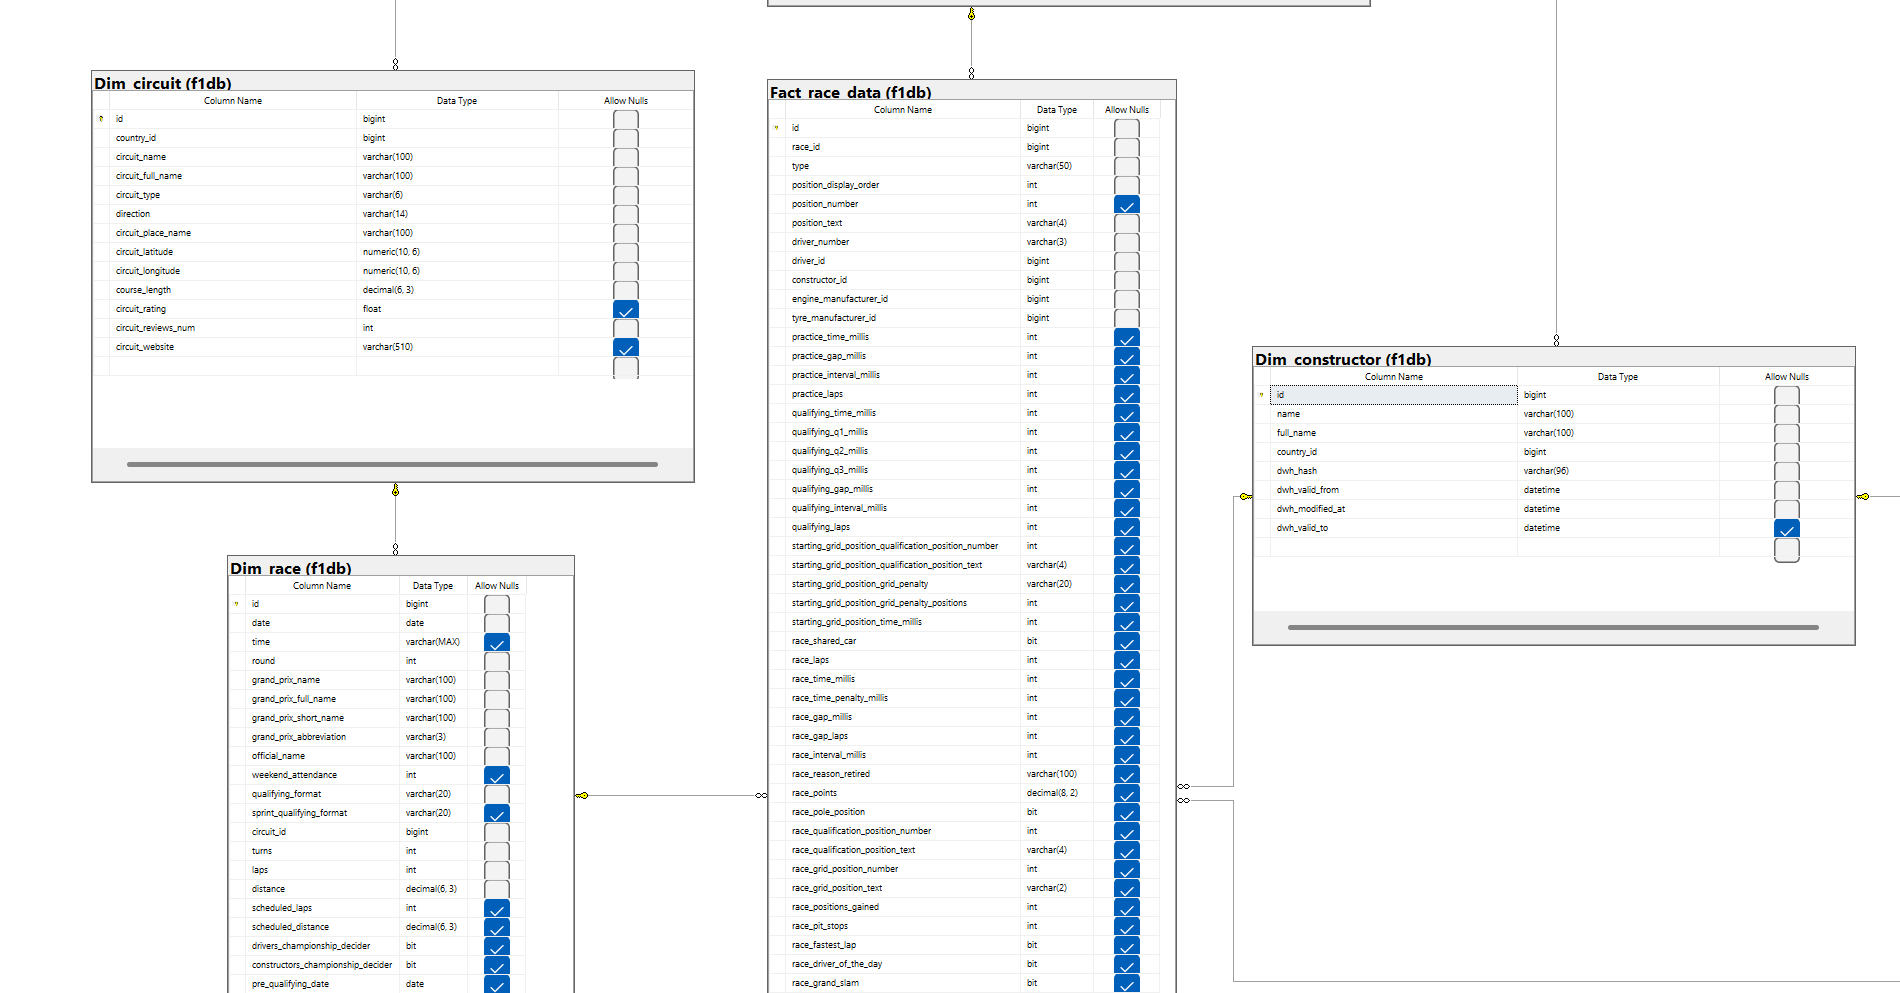
\includegraphics[width=\textwidth]{diagram3.png}
    \caption{Schemat hurtowni danych}
\end{figure}

\begin{figure}[H]
    \centering
    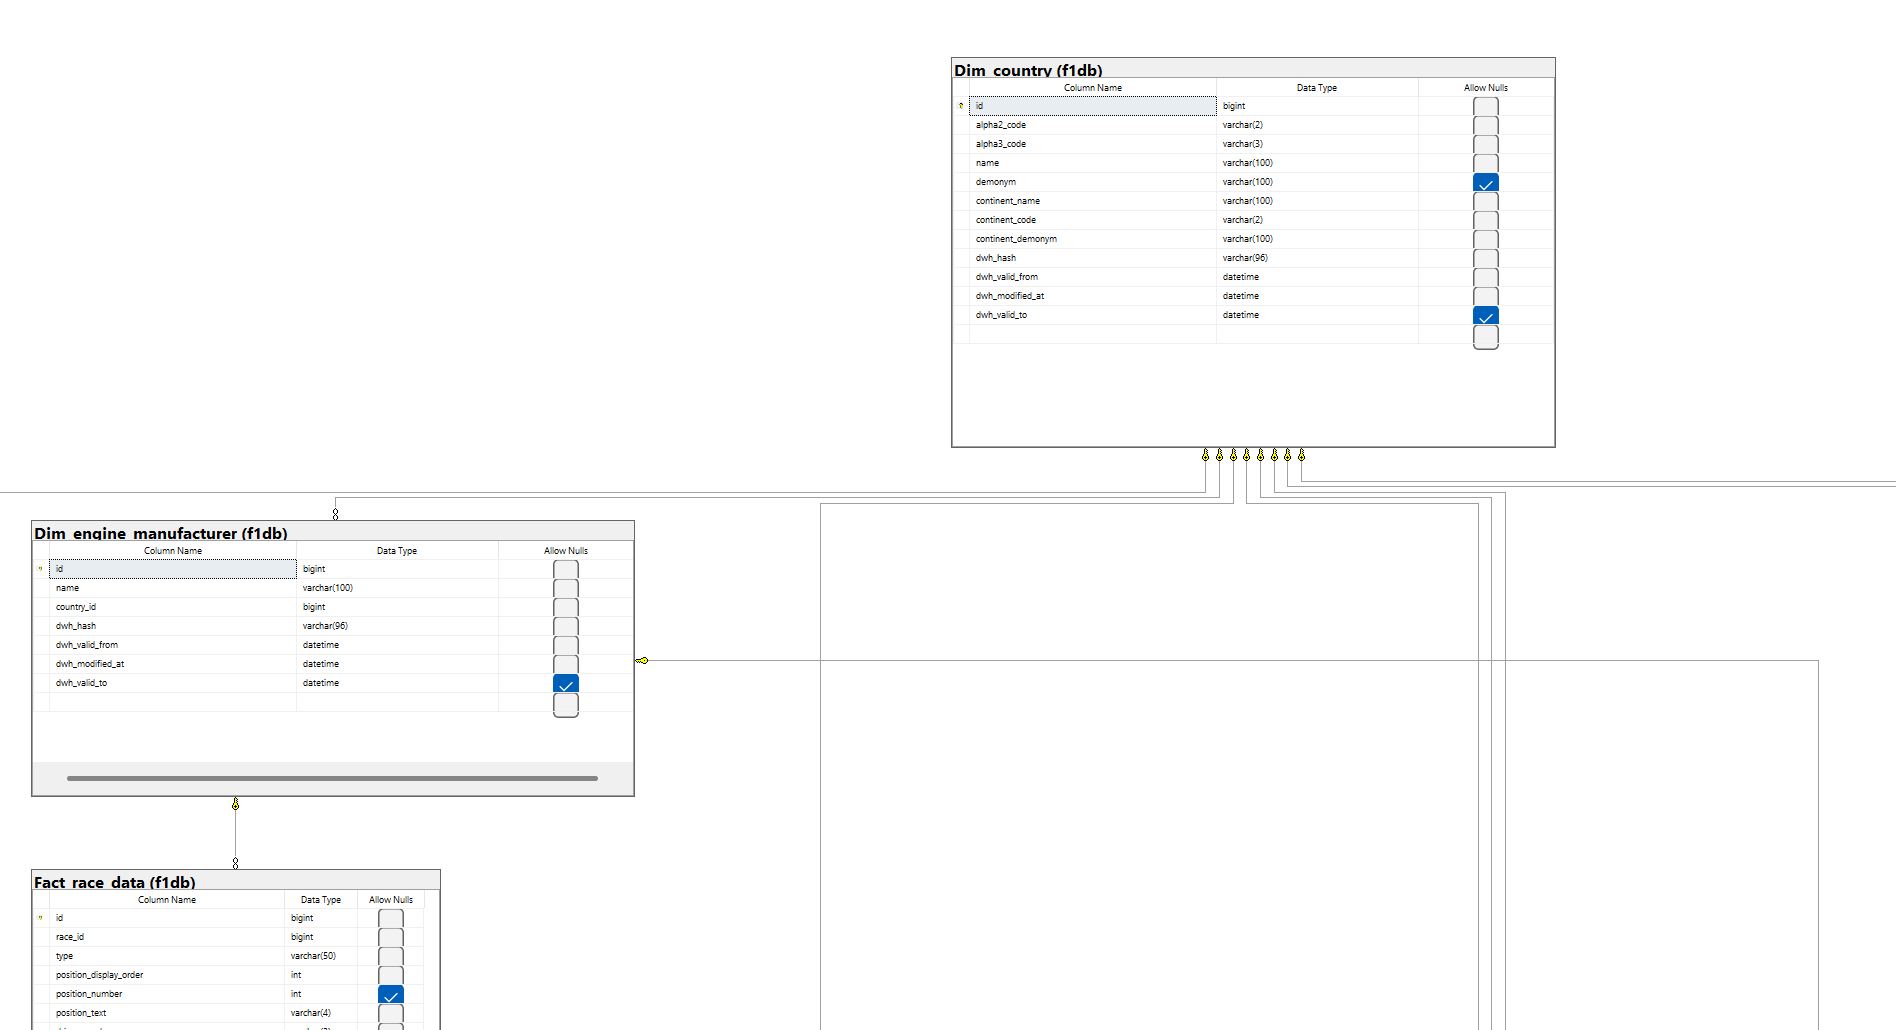
\includegraphics[width=\textwidth]{diagram4.png}
    \caption{Schemat hurtowni danych}
\end{figure}


\begin{figure}[H]
    \centering
    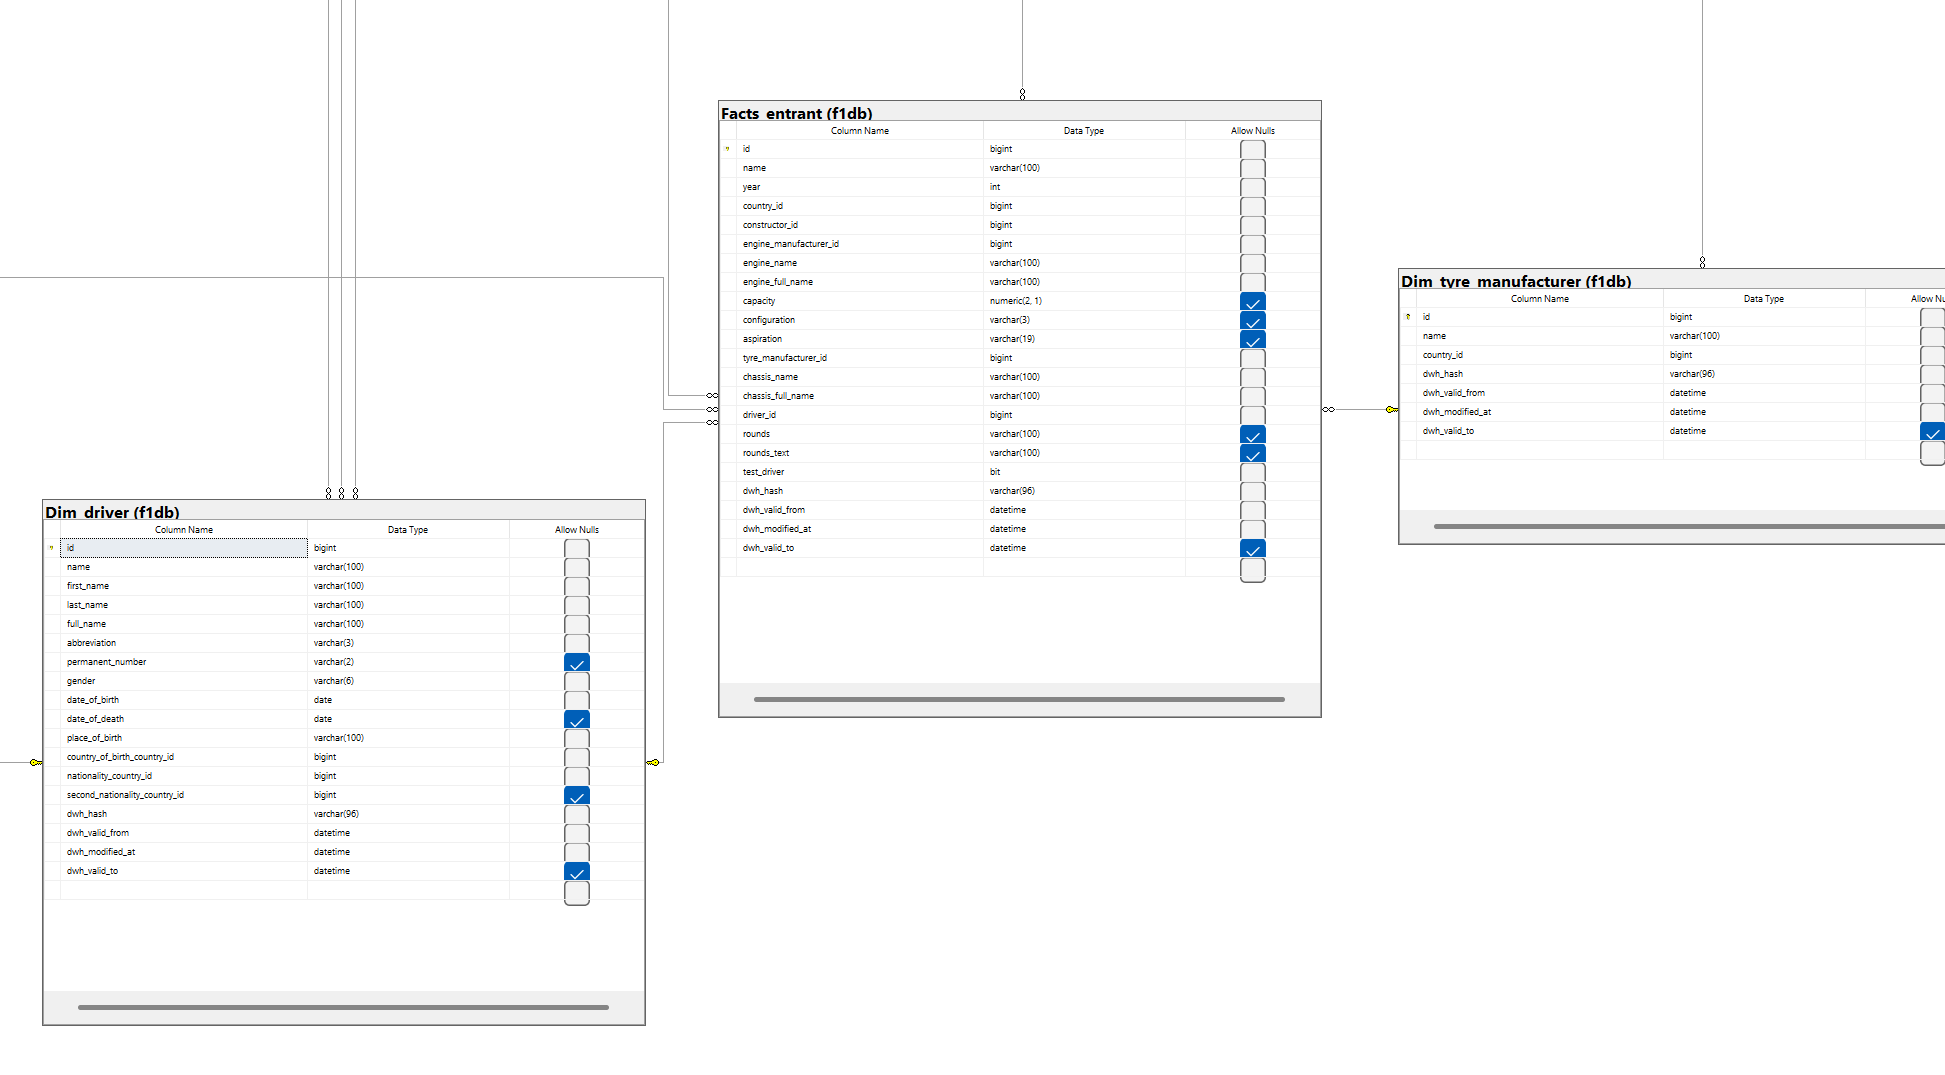
\includegraphics[width=\textwidth]{diagram5.png}
    \caption{Schemat hurtowni danych}
\end{figure}

Powyższy diagram stanowi fragment przykładowej wizualizacji struktury. Pełna implementacja została załączona jako skrypt SQL.

\section{Opis kluczowych miar i atrybutów}

\subsection{Tabele faktów}
Tabele faktów zawierają miary ilościowe, które są przedmiotem analiz. Poniżej przedstawiono główne tabele faktów wraz z opisem kluczowych miar.

\subsubsection{Fact\_race\_data}
\begin{longtable}{lp{8.5cm}}
\toprule
\textbf{Kolumna} & \textbf{Opis} \\
\midrule
\endhead

race\_id & Identyfikator wyścigu (klucz obcy do Dim\_race). \\
type & Typ sesji: race, qualifying, practice. \\
driver\_id & Identyfikator kierowcy (Dim\_driver). \\
constructor\_id & Identyfikator zespołu (Dim\_constructor). \\

race\_laps & Liczba ukończonych okrążeń. \\
race\_time\_millis & Całkowity czas wyścigu w milisekundach. \\
race\_gap\_millis & Różnica czasowa do lidera w milisekundach. \\
race\_positions\_gained & Liczba pozycji zyskanych względem startu. \\
race\_pit\_stops & Liczba pit stopów wykonanych w wyścigu. \\
race\_points & Punkty zdobyte za wyścig. \\
race\_fastest\_lap & Czy kierowca uzyskał najszybsze okrążenie (TAK/NIE). \\
race\_driver\_of\_the\_day & Czy kierowca został Driver of the Day. \\

qualifying\_time\_millis & Najlepszy czas kwalifikacyjny w milisekundach. \\
qualifying\_laps & Liczba okrążeń w kwalifikacjach. \\
starting\_grid\_position\_grid\_penalty\_positions & Liczba pozycji kary na starcie. \\

fastest\_lap\_time\_millis & Czas najszybszego okrążenia w milisekundach. \\
pit\_stop\_time\_millis & Czas trwania pit-stopu w milisekundach. \\
driver\_of\_the\_day\_percentage & Procent głosów oddanych na Driver of the Day. \\

\bottomrule
\caption{Najważniejsze miary i atrybuty w tabeli Fact\_race\_data}
\end{longtable}


\subsubsection{Facts\_entrant}
\begin{longtable}{lp{8.5cm}}
\toprule
\textbf{Kolumna} & \textbf{Opis} \\
\midrule
\endhead

id & Unikalny identyfikator zespołu. \\
name & Nazwa wyświetlana uczestnika. \\
year & Rok sezonu. \\
country\_id & Kraj uczestnika. \\
constructor\_id & Konstruktor. \\
engine\_manufacturer\_id & Producent silnika. \\
engine\_name & Skrócona nazwa silnika. \\
engine\_full\_name & Pełna nazwa silnika. \\
capacity & Pojemność silnika w litrach. \\
configuration & Konfiguracja silnika (np. V6, V8). \\
aspiration & Typ doładowania (np. Turbo, N/A). \\
tyre\_manufacturer\_id & Producent opon. \\
chassis\_name & Skrócona nazwa nadwozia. \\
chassis\_full\_name & Pełna nazwa nadwozia. \\
driver\_id & Identyfikator przypisanego kierowcy. \\
rounds & Numery rund, w których uczestniczył kierowca. \\
rounds\_text & Opis tekstowy rund. \\
test\_driver & Czy kierowca był testowym/rezerwowym. \\

\bottomrule
\caption{Najważniejsze miary i atrybuty w tabeli Facts\_entrant}
\end{longtable}

\subsection{Tabele wymiarów}
Tabele wymiarów zawierają atrybuty opisujące kontekst, którego dotyczą miary w tabelach faktów.

\subsubsection{Dim\_constructor}
\begin{longtable}{lp{8.5cm}}
\toprule
\textbf{Kolumna} & \textbf{Opis} \\
\midrule
\endhead

id & Unikalny identyfikator konstruktora. \\
name & Skrócona nazwa konstruktora. \\
full\_name & Pełna oficjalna nazwa konstruktora. \\
country\_id & Kraj pochodzenia konstruktora. \\

\bottomrule
\caption{Najważniejsze miary i atrybuty w tabeli Dim\_constructor}
\end{longtable}

\subsubsection{Dim\_driver}
\begin{longtable}{lp{8.5cm}}
\toprule
\textbf{Kolumna} & \textbf{Opis} \\
\midrule
\endhead

id & Unikalny identyfikator kierowcy. \\
full\_name & Pełne imię i nazwisko kierowcy. \\
abbreviation & Skrót nazwiska kierowcy (3 litery). \\
gender & Płeć kierowcy. \\
date\_of\_birth & Data urodzenia kierowcy. \\
country\_of\_birth\_country\_id & Kraj urodzenia kierowcy. \\
nationality\_country\_id & Główna narodowość kierowcy. \\


\bottomrule
\caption{Najważniejsze miary i atrybuty w tabeli Dim\_driver}
\end{longtable}

\subsubsection{Dim\_engine\_manufacturer}
\begin{longtable}{lp{8.5cm}}
\toprule
\textbf{Kolumna} & \textbf{Opis} \\
\midrule
\endhead

id & Unikalny identyfikator producenta silników. \\
name & Nazwa producenta silników. \\
country\_id & Kraj producenta silników. \\


\bottomrule
\caption{Najważniejsze miary i atrybuty w tabeli Dim\_engine\_manufacturer}
\end{longtable}

\subsubsection{Dim\_race}
\begin{longtable}{lp{8.5cm}}
\toprule
\textbf{Kolumna} & \textbf{Opis} \\
\midrule
\endhead

id & Unikalny identyfikator wyścigu. \\
year & Rok rozegrania wyścigu. \\
round & Numer wyścigu w sezonie. \\
date & Data wyścigu. \\
time & Godzina rozpoczęcia wyścigu. \\
grand\_prix\_name & Nazwa Grand Prix. \\
grand\_prix\_full\_name & Pełna nazwa Grand Prix. \\
grand\_prix\_short\_name & Skrócona nazwa Grand Prix. \\
grand\_prix\_abbreviation & Trzyliterowy skrót Grand Prix. \\
country\_id & Identyfikator kraju, w którym odbywa się wyścig. \\
official\_name & Oficjalna nazwa wydarzenia. \\
weekend\_attendance & Frekwencja podczas weekendu wyścigowego. \\
qualifying\_format & Format kwalifikacji. \\
sprint\_qualifying\_format & Format kwalifikacji sprinterskich. \\


\bottomrule
\caption{Atrybuty wymiaru wyścigu w tabeli Dim\_race}
\end{longtable}


\section{Opis warstwy raportowej}

Warstwa raportowa w hurtowni danych dla środowiska Formuły 1 odgrywa kluczową rolę w prezentacji przetworzonych informacji użytkownikom końcowym – analitykom, strategom zespołów, mediom oraz organizatorom. Zapewnia ona ustrukturyzowany i zrozumiały dostęp do danych poprzez zdefiniowane modele biznesowe, przekształcenia oraz hierarchie.

\subsection*{Dostęp do danych}

Użytkownicy uzyskują dostęp do warstwy raportowej za pośrednictwem:
\begin{itemize}
    \item narzędzia analitycznego Power BI,
\end{itemize}
które umożliwia interaktywne przeglądanie raportów, wizualizację danych oraz wykonywanie zapytań ad hoc. Dostęp do informacji jest kontrolowany w oparciu o system ról i uprawnień.

\subsection*{Model biznesowy danych}

Model danych oparty jest na schemacie galaktyki (ang. \textit{galaxy schema}). Główne fakty to:
\begin{itemize}
    \item \texttt{Fact\_race\_data} – szczegółowe dane wyścigowe,
    \item \texttt{Fact\_entrant} – dane związane z udziałem bolidów i kierowców w wyścigach.
\end{itemize}
Modele te są otoczone przez odpowiednie wymiary, takie jak czas, tor, kierowca, zespół czy lokalizacja, umożliwiając tworzenie zaawansowanych analiz przekrojowych.

\subsection*{Transformacje w obrębie warstwy raportowej}

Transformacje stosowane w warstwie raportowej umożliwiają prezentację danych w formie zoptymalizowanej pod kątem raportowania i analizy. Wśród kluczowych transformacji znajdują się:
\begin{itemize}
    \item obliczanie skumulowanej liczby punktów w obrębie sezonu,
    \item formatowanie czasu trwania pit stopów,
    \item oznaczenie ostatniego rozegranego wyścigu,
    \item identyfikacja najbliższego zaplanowanego wyścigu,
    \item określenie, czy kierowca znalazł się na podium w danym wyścigu,
    \item agregacja i formatowanie łącznego czasu ukończenia wyścigu,
    \item obliczenia zagregowanej oraz średniej oglądalności wyścigów,
    \item porównania oglądalności sezonów (wzrosty/spadki),
    \item wyodrębnienie roku wyścigu z daty wydarzenia,
    \item sumowanie liczby miejsc na podium i zwycięstw danego kierowcy,
    \item kalkulacja łącznych punktów kierowców oraz zespołów w sezonie,
    \item oznaczenie, czy wyścig się odbył oraz czy należy do najbliższych Grand Prix.
\end{itemize}

\section{Realizacja przykładowych raportów}

\subsection*{1. Rankingi}

\textbf{Cel:} Prezentacja bieżącej klasyfikacji kierowców i zespołów.\\
\textbf{Zakres:}
\begin{itemize}
    \item klasyfikacja kierowców w danym sezonie,
    \item klasyfikacja zespołów w danym sezonie,
    \item wykres przedstawiający zmiany punktacji kierowców w trakcie sezonu,
    \item ranking popularności kierowców na podstawie danych demograficznych i interakcji fanów.
\end{itemize}

\subsection*{2. Kierowcy}

\textbf{Cel:} Analiza osiągnięć i kariery poszczególnych kierowców.\\
\textbf{Zakres:}
\begin{itemize}
    \item wyszukiwanie kierowców według imienia i nazwiska,
    \item liczba zdobytych punktów,
    \item narodowość i data urodzenia,
    \item liczba miejsc na podium,
    \item liczba zwycięstw w wyścigach.
\end{itemize}

\subsection*{3. Tory i oglądalność wyścigów}

\textbf{Cel:} Analiza atrakcyjności poszczególnych torów na podstawie danych oglądalności.\\
\textbf{Zakres:}
\begin{itemize}
    \item łączna i średnia oglądalność w sezonie,
    \item mapa torów wyścigowych zawierająca:
    \begin{itemize}
        \item długość toru,
        \item datę nadchodzącego Grand Prix,
        \item link do oficjalnej strony toru.
    \end{itemize}
\end{itemize}

\subsection*{4. Terminarz wyścigów}

\textbf{Cel:} Ułatwienie śledzenia przebiegu sezonu dla kibiców oraz użytkowników komercyjnych.\\
\textbf{Zakres:}
\begin{itemize}
    \item liczba zakończonych i planowanych wyścigów w sezonie,
    \item szczegóły dotyczące najbliższego wyścigu (data, lokalizacja),
    \item mapa torów wraz z podziałem geograficznym (kontynenty),
    \item wyniki ostatniego rozegranego wyścigu.
\end{itemize}

\subsection*{5. Przegląd zespołów}

\textbf{Cel:} Przedstawienie danych technicznych bolidów oraz efektywności operacyjnej zespołów.\\
\textbf{Zakres:}
\begin{itemize}
    \item szczegóły techniczne dotyczące podwozia i silnika bolidu,
    \item wizualizacja modelu bolidu,
    \item wykresy czasu pit-stopów z podziałem na zespoły i wyścigi.
\end{itemize}

\section{Wizualizacja raportu}

Poniżej znajdują się zdjęcia ilustrujące wygląd raportu w \textit{Power BI}.

\begin{figure}[H]
    \centering
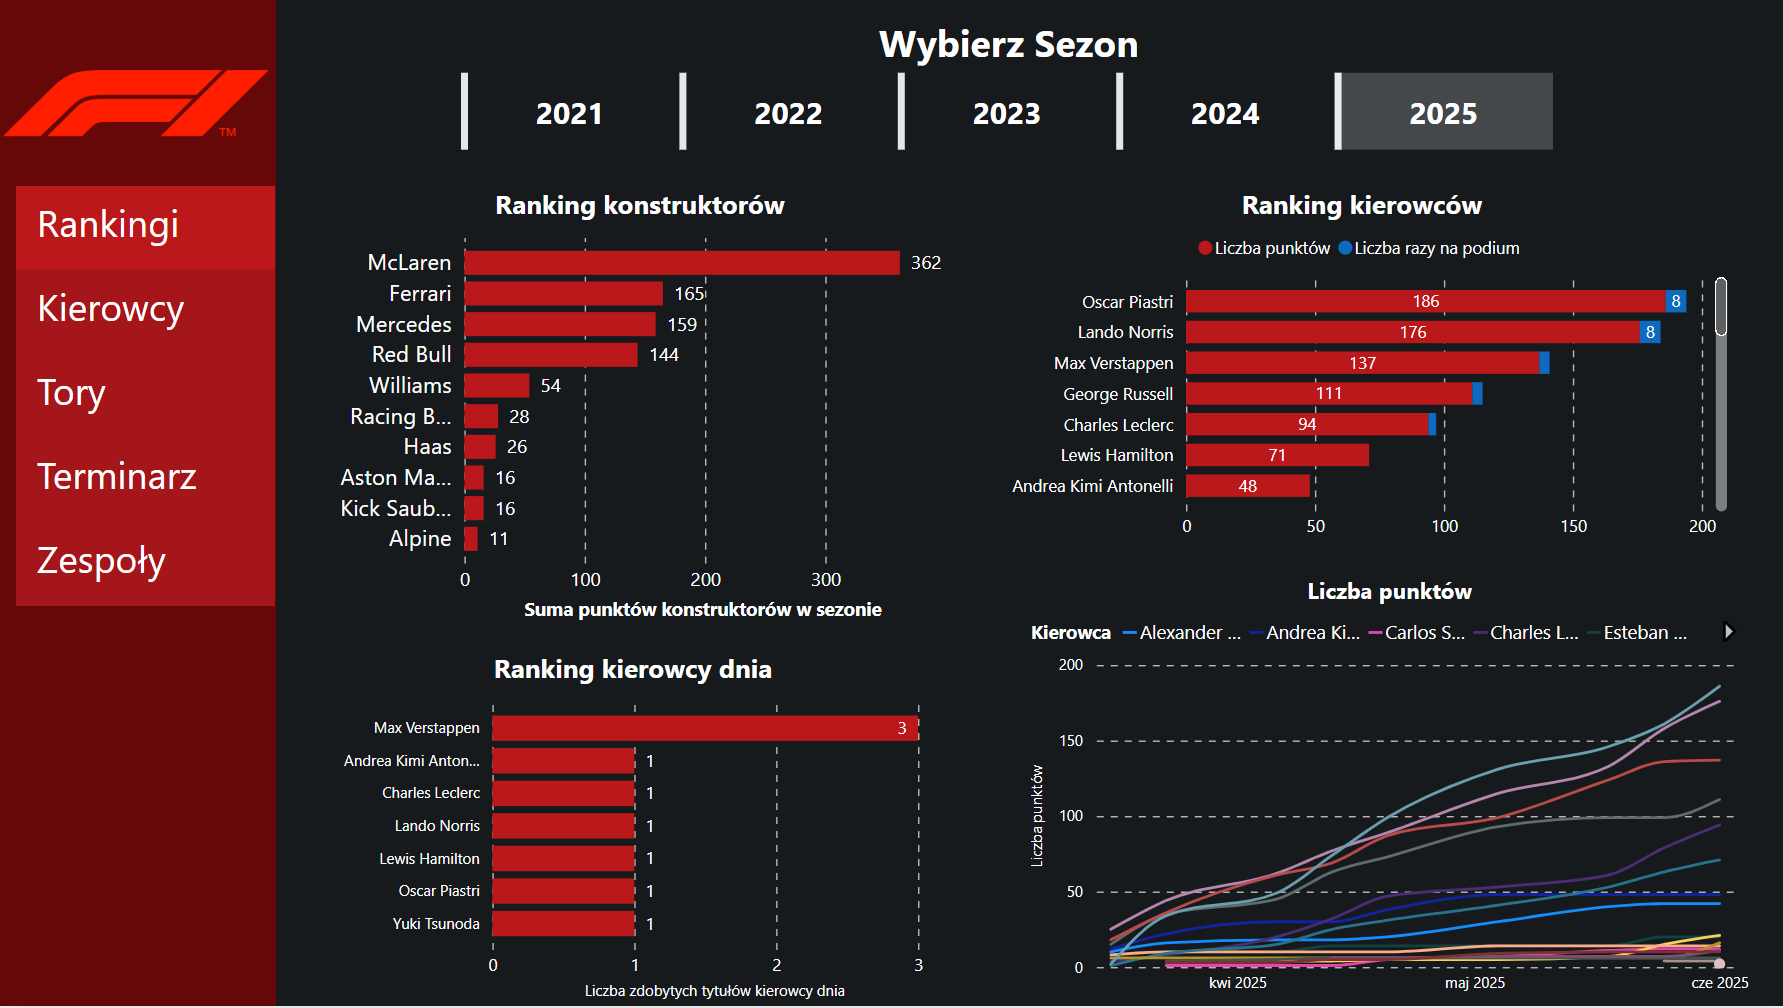
\includegraphics[width=\textwidth]{raport1.png}
    \caption{Strona przedstawiająca aktualne rankingi kierowców i zespołów, wraz z wizualizacją zmian punktacji w trakcie sezonu oraz analizą popularności wśród fanów.}
\end{figure}

\begin{figure}[H]
    \centering
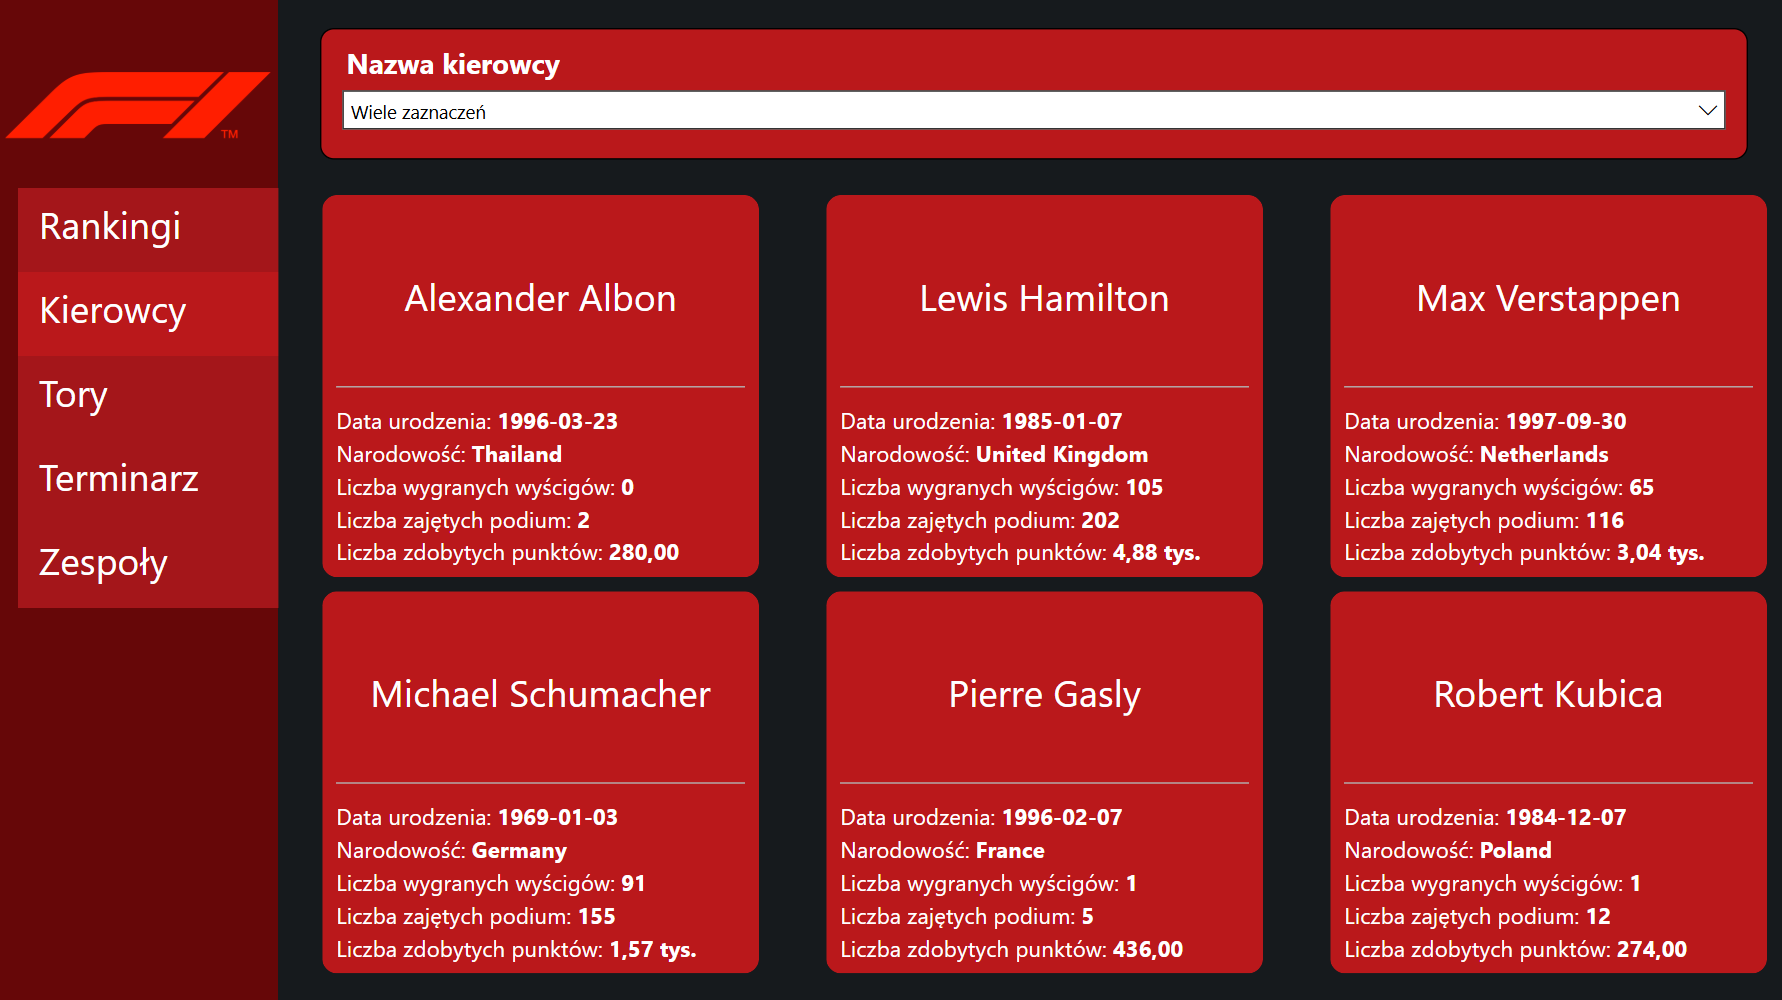
\includegraphics[width=\textwidth]{raport2.png}
    \caption{Widok umożliwiający przegląd i porównanie kierowców, ich statystyk, narodowości, liczby zwycięstw i miejsc na podium.}
\end{figure}


\begin{figure}[H]
    \centering
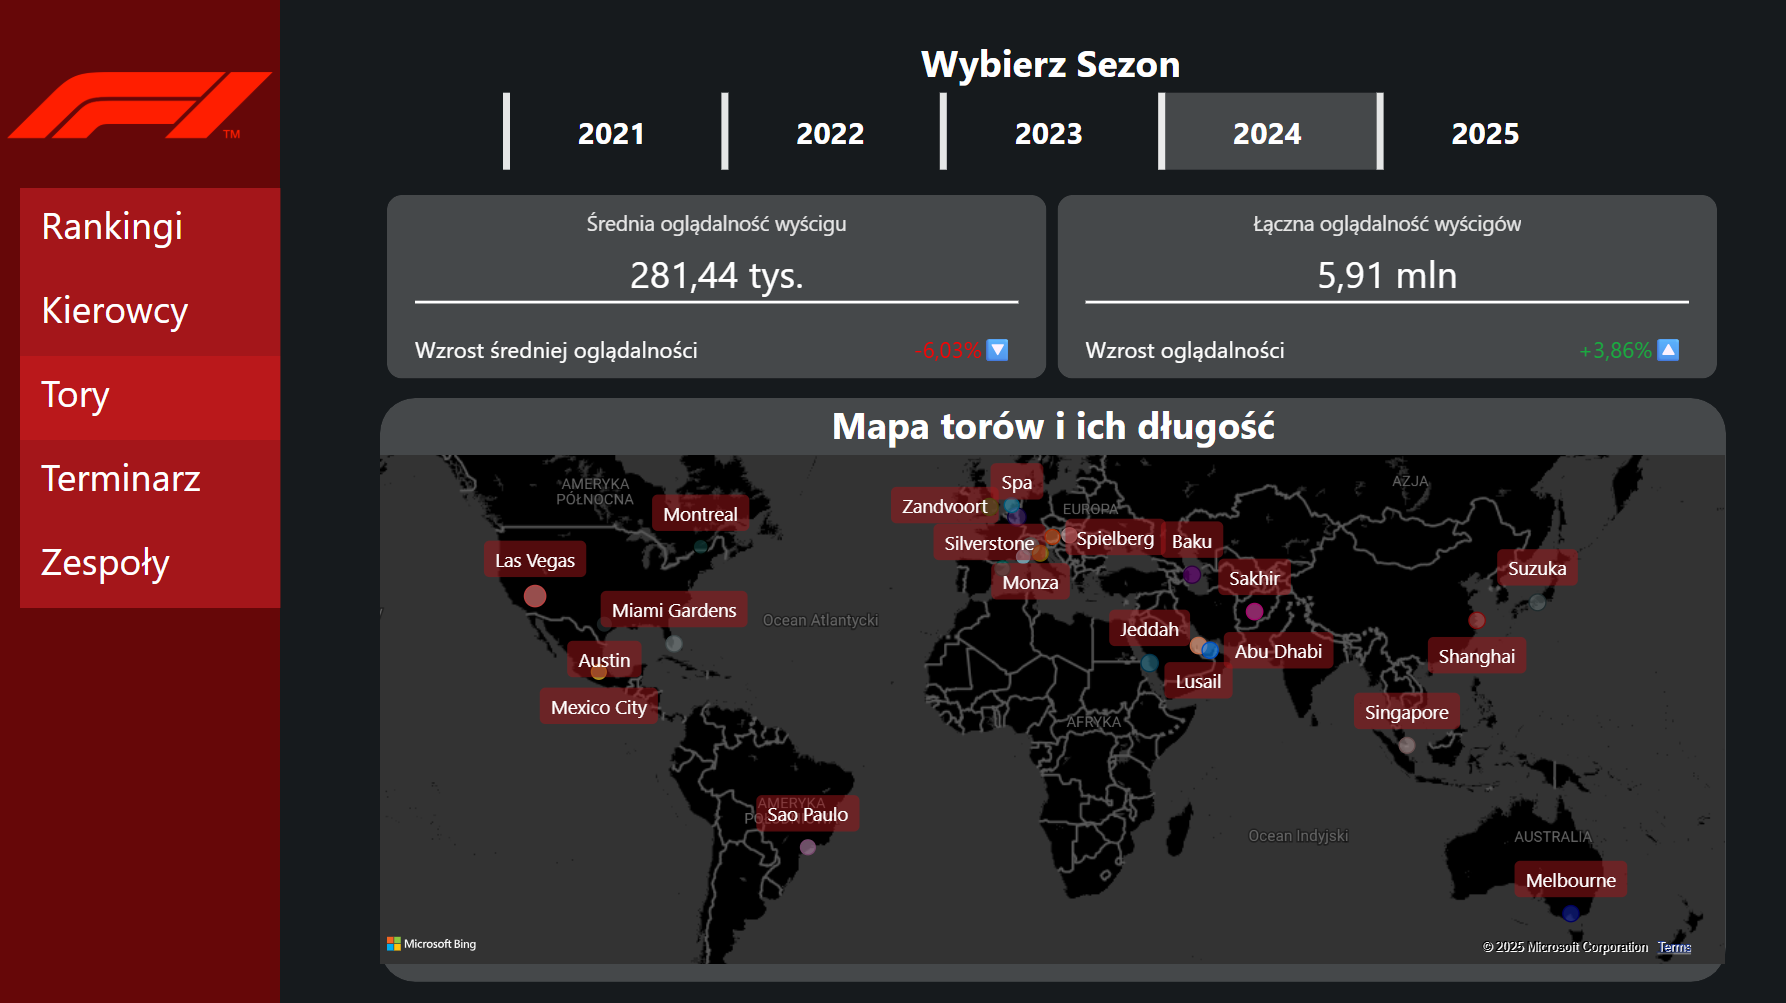
\includegraphics[width=\textwidth]{raport3.png}
    \caption{Strona z mapą torów wyścigowych i szczegółami dotyczącymi długości torów, nadchodzących wydarzeń oraz statystyk oglądalności.}
\end{figure}

\begin{figure}[h!]
    \centering
    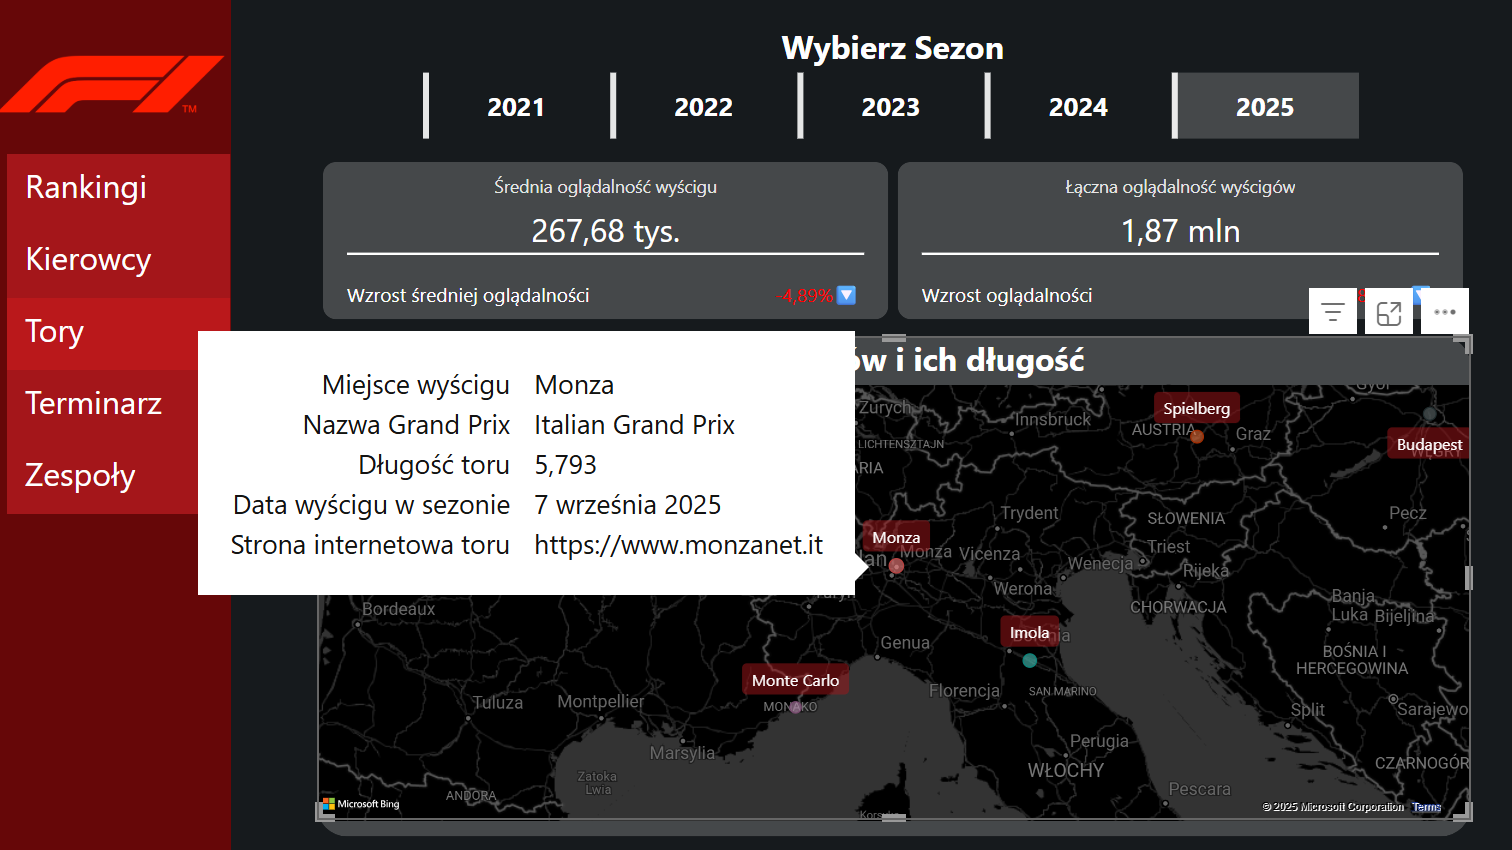
\includegraphics[width=0.95\textwidth]{ab.png}
    \caption{Strona z mapą torów wyścigowych i szczegółami dotyczącymi długości torów, nadchodzących wydarzeń oraz statystyk oglądalności.}
\end{figure}


\begin{figure}[H]
    \centering
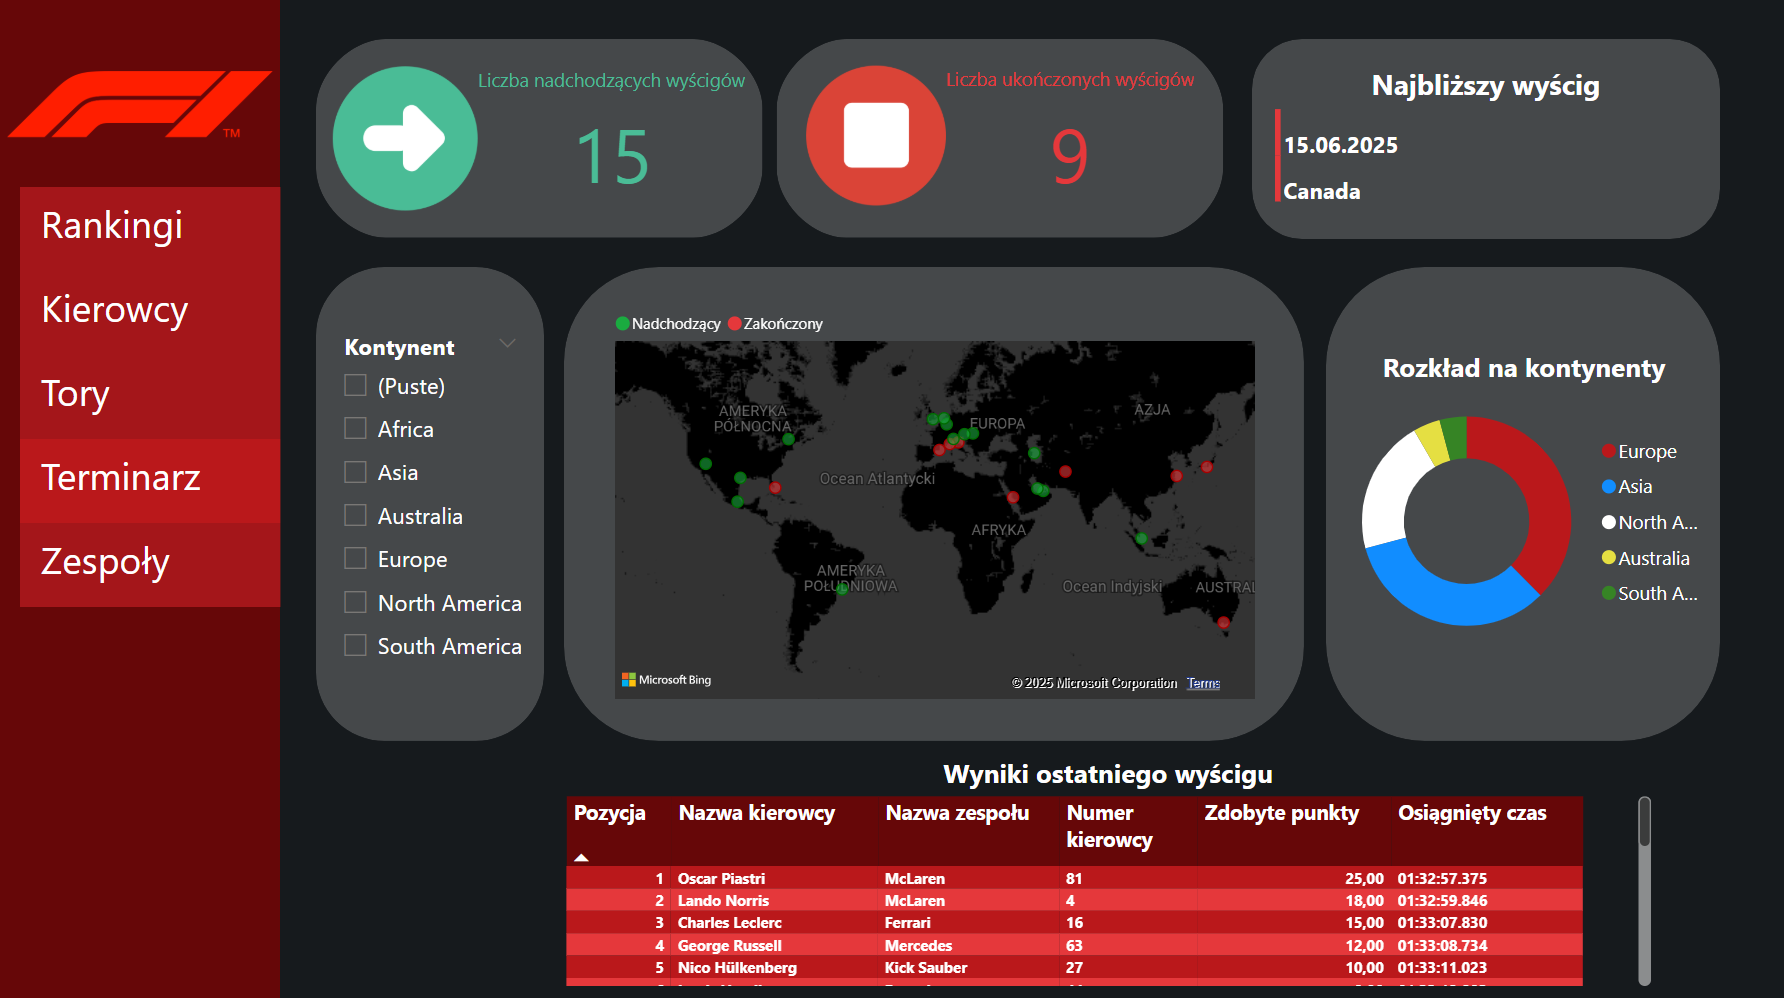
\includegraphics[width=\textwidth]{raport4.png}
    \caption{Zestawienie zakończonych i planowanych wyścigów w sezonie, uzupełnione mapą lokalizacji i wynikami ostatniego Grand Prix.}
\end{figure}


\begin{figure}[H]
    \centering
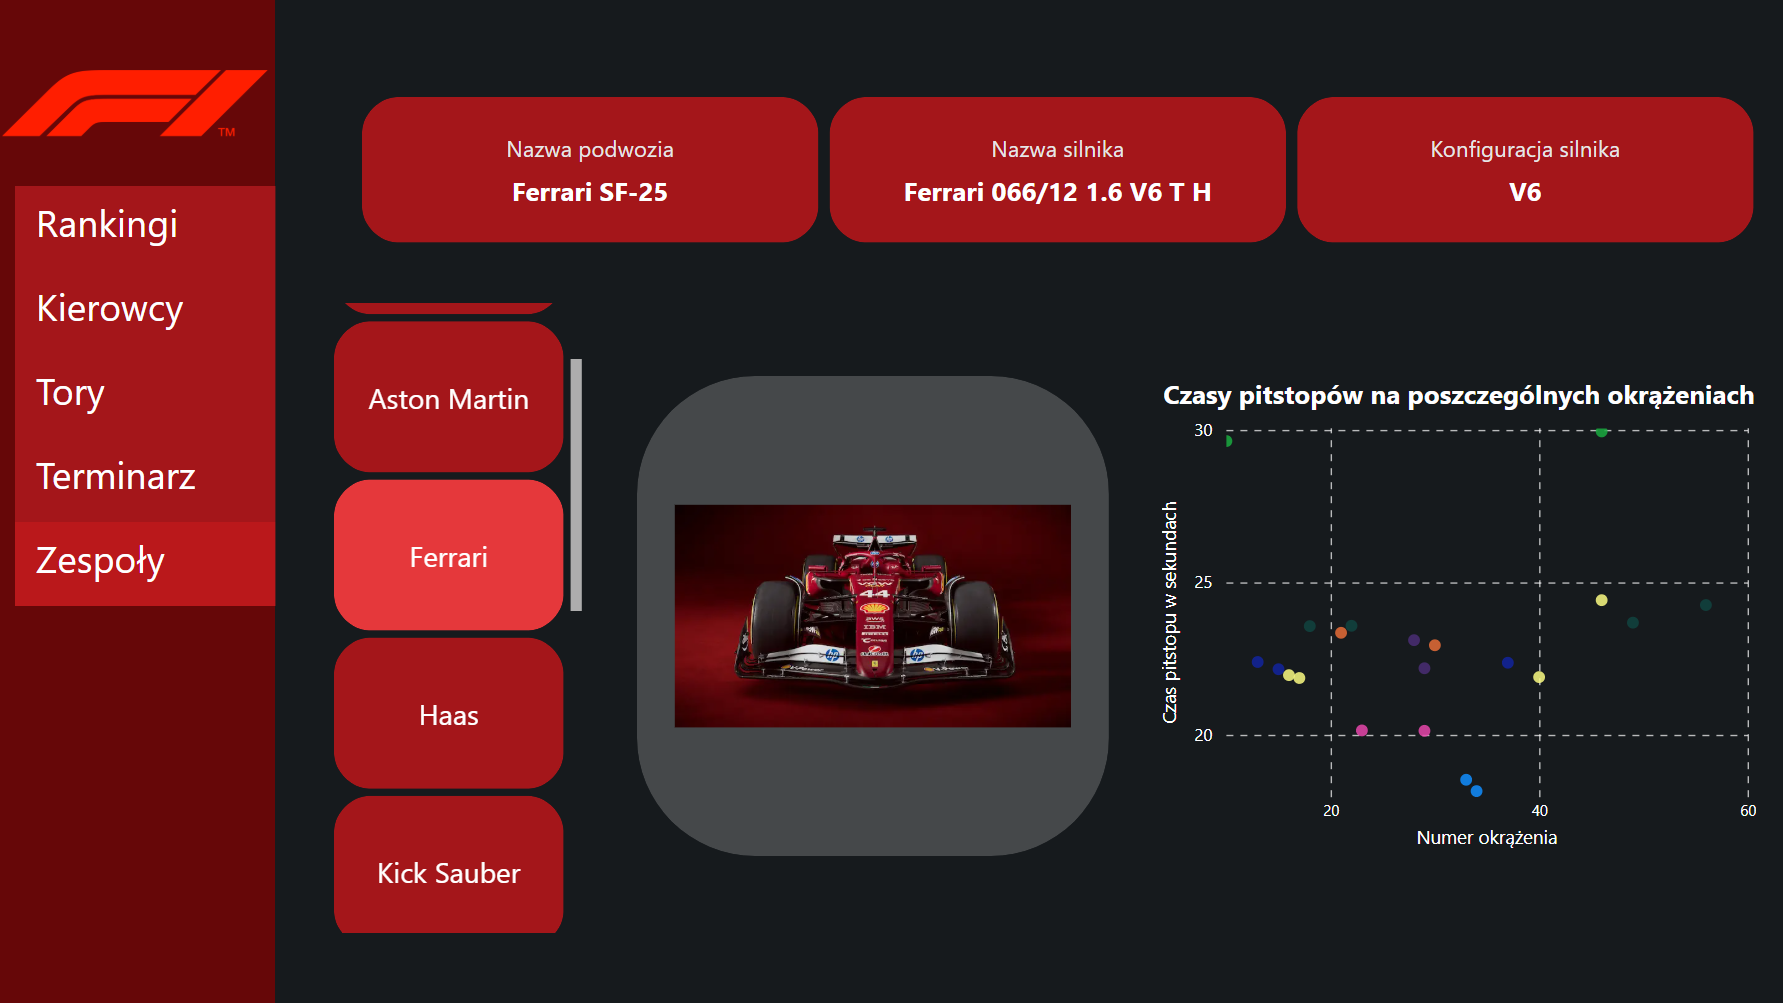
\includegraphics[width=\textwidth]{raport5.png}
    \caption{Prezentacja danych technicznych bolidów, wizualizacji modeli oraz analiz czasów pit-stopów dla każdego zespołu.}
\end{figure}

\section{Podsumowanie rezultatów projektu}

Zrealizowany projekt budowy hurtowni danych dla środowiska Formuły 1 dostarczył kompleksowe i skalowalne rozwiązanie wspierające analizę wyników sportowych, planowanie strategiczne oraz komunikację z interesariuszami. Na podstawie przeprowadzonych testów oraz przykładowych raportów można wskazać szereg korzyści biznesowych wynikających z wdrożenia systemu:

\begin{itemize}
    \item \textbf{Wzrost efektywności analizy danych:} Integracja danych z różnych źródeł (wyniki wyścigów, statystyki kierowców, oglądalność, dane o torach) umożliwiła tworzenie przekrojowych raportów wspomagających decyzje analityków i strategów zespołów.

    \item \textbf{Usprawnienie raportowania:} Zcentralizowana warstwa raportowa pozwala na automatyzację procesu tworzenia raportów dla sponsorów, federacji oraz mediów, co znacząco skraca czas przygotowania analiz sezonowych i bieżących.

    \item \textbf{Lepsze planowanie strategiczne:} Dzięki wdrożeniu zaawansowanych transformacji danych i wskaźników (np. rankingów, wzrostów/spadków oglądalności, formy kierowców), możliwe jest podejmowanie trafniejszych decyzji dotyczących składu zespołów, logistyki czy marketingu.

    \item \textbf{Wsparcie zaangażowania kibiców:} Raporty prezentujące terminarz, lokalizacje torów, dane historyczne oraz nadchodzące wyścigi umożliwiają tworzenie atrakcyjnych i angażujących treści dla fanów motorsportu.

    \item \textbf{Elastyczność i skalowalność:} Zastosowana architektura hurtowni danych pozwala na łatwe rozszerzenie systemu o dodatkowe źródła danych oraz nowe raporty.
\end{itemize}

Pod względem biznesowym projekt spełnił swoje cele, zapewniając wartość dodaną zarówno dla użytkowników operacyjnych, jak i decyzyjnych. Przyjęte rozwiązania wspierają rozwój analityki w organizacji oraz budowanie przewagi konkurencyjnej w sektorze sportów motorowych.


\section{Testy}
\subsection{Testowanie ręczne z Prefect Deployment}
W ramach testów, osoba odpowiedzialna za nadzór powinna okresowo monitorować tablicę z wynikami, aby upewnić się, że wszystkie zadania wykonują się zgodnie z planem. Dodatkowo, powiadomienia mailowe zostały skonfigurowane, aby informować zespół o statusie zadań.

\subsection{Proces Deploymentu}
Deployment w systemie jest wykonywany na podstawie kilku zadań (tasks), które są uruchamiane zgodnie z harmonogramem. Każdy task jest odpowiedzialny za wykonanie konkretnego etapu procesu, np. klonowanie repozytorium, instalowanie zależności, uruchamianie skryptów ELT, itp.

Harmonogram uruchamiania jest zarządzany przez Prefect, który obsługuje wszystkie zadania (tasks) w ramach deploymentu, zgodnie z poniższymi ustawieniami.

\subsection{Zadania w deploymentach}
\subsubsection{test-flow}
\begin{itemize}
    \item \textbf{Cel:} Testowanie połączeń oraz sprawdzenie poprawności uruchamiania zadań w systemie.
    \item \textbf{Harmonogram:} Ręczne uruchomienie zadania.
    \item \textbf{Opis:} Task testowy uruchamiany ręcznie w celu weryfikacji, czy wszystkie połączenia (np. do bazy danych, repozytorium GitHub) działają prawidłowo.
    \item \textbf{Kroki:}
    \begin{itemize}
        \item Klonowanie repozytorium z GitHub.
        \item Instalowanie wymaganych zależności.
        \item Uruchomienie testów (np. testów jednostkowych lub połączeń).
    \end{itemize}

\end{itemize}

\subsubsection{racing-circuits}
\begin{itemize}
    \item \textbf{Cel:} Uruchomienie procesu ETL dla danych o torach wyścigowych.
    \item \textbf{Harmonogram:} Uruchamiane co miesiąc o godzinie 3:00 w pierwszym dniu miesiąca.
    \item \textbf{Opis:} Pobieranie danych o torach wyścigowych, przetwarzanie ich i ładowanie do systemu.
    \item \textbf{Cron:} \texttt{0 3 1 * *} (co miesiąc, 3:00 AM, 1 dnia)
\end{itemize}

\subsubsection{f1\_attandance}
\begin{itemize}
    \item \textbf{Cel:} Uruchomienie procesu ETL dla danych o obecności.
    \item \textbf{Harmonogram:} Uruchamiane co poniedziałek o godzinie 3:00.
    \item \textbf{Opis:} Pobieranie danych o obecności kibiców i ich wprowadzenie do bazy danych.
    \item \textbf{Cron:} \texttt{0 3 * * 1} (co tydzień, poniedziałek, 3:00 AM)
\end{itemize}

\subsubsection{f1db}
\begin{itemize}
    \item \textbf{Cel:} Przesyłanie danych do bazy danych F1.
    \item \textbf{Harmonogram:} Uruchamiane co poniedziałek o godzinie 3:00.
    \item \textbf{Opis:} Proces ETL do przesyłania danych do bazy danych.
    \item \textbf{Cron:} \texttt{0 3 * * 1} (co tydzień, poniedziałek, 3:00 AM)
\end{itemize}

\subsection{DWH}
\begin{itemize}
    \item \textbf{Cel:} Przeprowadzenie procesu ETL dla danych z naszej bazy F1DB do naszej hurtowni danych F1DWH.
    \item \textbf{Harmonogram:} Uruchamiane co poniedziałek o godzinie 5:00.
    \item \textbf{Opis:} Proces ETL danych z bazy do hurtowni danych.
    \item \textbf{Cron:} \texttt{0 5 * * 1} (co tydzień, poniedziałek, 5:00 AM)
    \item \textbf{Test:}
    Test w postaci logów czy dane zostały załadowane w poprawny sposób.
    \begin{figure}[H]
    \centering
    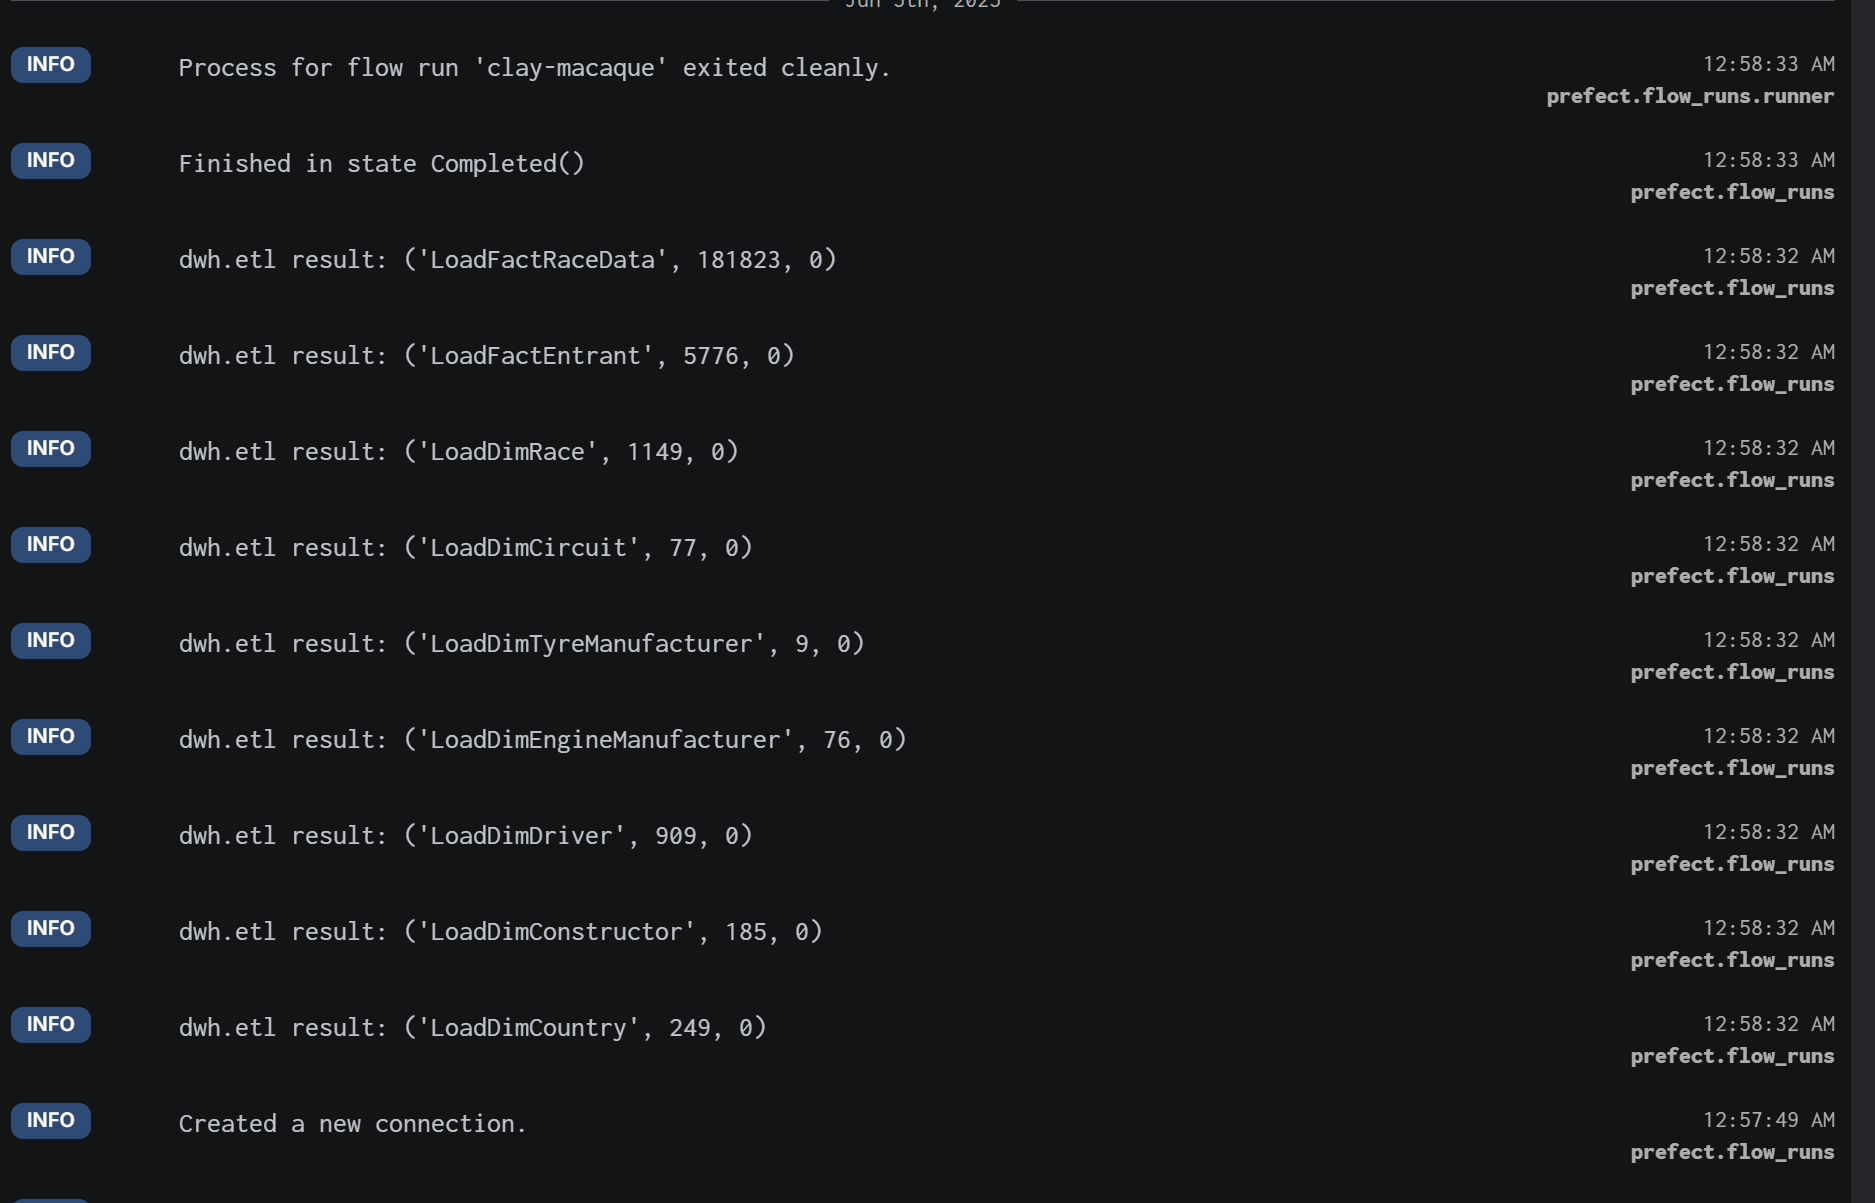
\includegraphics[width=\textwidth]{test1.png}
    \caption{Logi dla tego procesu}
\end{figure}

\end{itemize}

\begin{figure}[H]
    \centering
    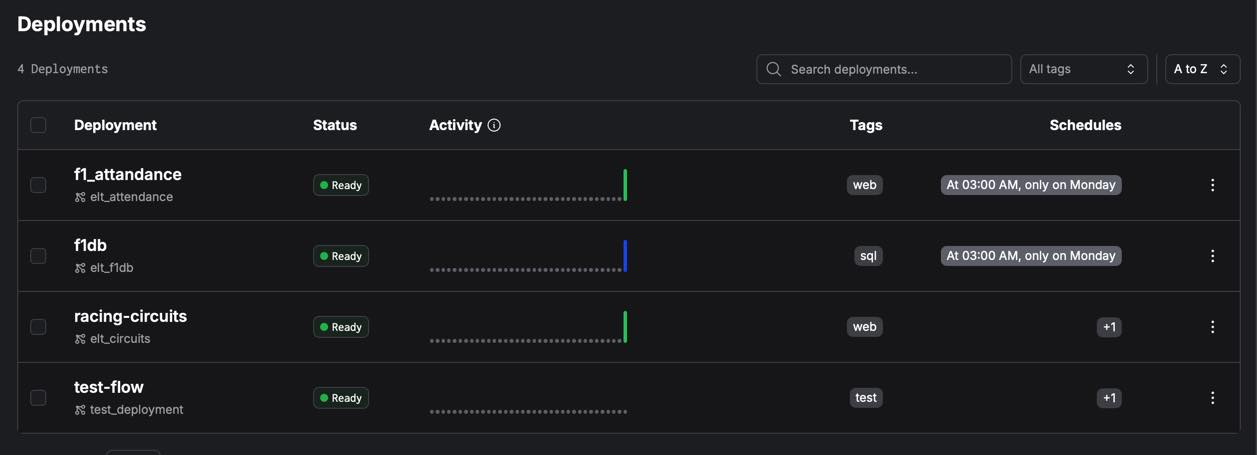
\includegraphics[width=\textwidth]{sc3.jpg}
    \caption{Zaplanowane procesy}
\end{figure}

\subsection{Testowanie jakościowe kodu}

Aby zapewnić, że system będzie rozwijalny, łatwy w utrzymaniu i niezawodny, przeprowadzono również testy jakościowe kodu. Testy te koncentrują się na trzech kluczowych aspektach: poprawności typów danych, formatowaniu kodu oraz dokumentacji. Poniżej przedstawiono szczegóły tych testów.

\subsubsection{Testowanie poprawności typów danych}

Testy sprawdzają, czy kod gwarantuje poprawność typów danych oraz unika niejawnych rzutowań (castów), które mogłyby prowadzić do błędów w działaniu systemu. Kluczowe kroki w tym procesie to:
\begin{itemize}
    \item \textbf{Sprawdzanie deklaracji typów:} Weryfikacja, czy zmienne są odpowiednio zadeklarowane z właściwymi typami danych. Na przykład, zmienne przechowujące liczby całkowite powinny być deklarowane jako \texttt{int}, a zmienne przechowujące dane tekstowe jako \texttt{str}.
    \item \textbf{Brak niejawnych rzutowań:} Zapewnienie, że w kodzie nie występują niejawne rzutowania danych, takie jak konwersja zmiennych typu \texttt{str} do \texttt{int} czy \texttt{float} bez jawnej weryfikacji poprawności. Każda konwersja powinna być wyraźnie zdefiniowana w kodzie, aby uniknąć nieoczekiwanych błędów.
\end{itemize}

\subsubsection{Testowanie formatowania kodu}

Testy formatowania kodu mają na celu zapewnienie spójności i zgodności przy dalszym rozwoju hurtowni.

\subsection{Testy z wykorzystaniem constraints}

W ramach testowania bazy danych wykorzystaliśmy system constraintów w celu weryfikacji poprawności wprowadzanych danych.

\subsubsection{1. Przykłady constraintów na bazie danych}

Przykład constraintu na bazie danych:
\begin{itemize}
    \item \textbf{Constraint UNIQUE:} Zapewnienie, że wartości w określonej kolumnie są unikalne. Na przykład, w tabeli krajów, nazwa kraju musi być unikalna
    \begin{verbatim}
    UniqueConstraint("name", name="uq_country_name")
    \end{verbatim}
    \item \textbf{Constraint CHECK:} Weryfikacja, że wartości w kolumnie spełniają określony warunek. Na przykład, pozycja w wyścigu musi być większa, bądź równa 1 i nie może być NULL.
    \begin{verbatim}
    CheckConstraint(
            "position_number IS NULL OR position_number >= 1",
            name="check_sem_position_number_min",
        ),
    \end{verbatim}
\end{itemize}

\subsection{Testowanie Scrappingu}

Podczas procesu scrappingu danych, kluczowe jest, aby wszystkie dane były zbierane w oczekiwanym formacie i z odpowiednimi typami danych. Każdy scrapowany element jest walidowany pod kątem oczekiwanego typu danych oraz struktury.


\subsection{Zdjęcia przedstawiające działanie}
\begin{figure}[H]
    \centering
    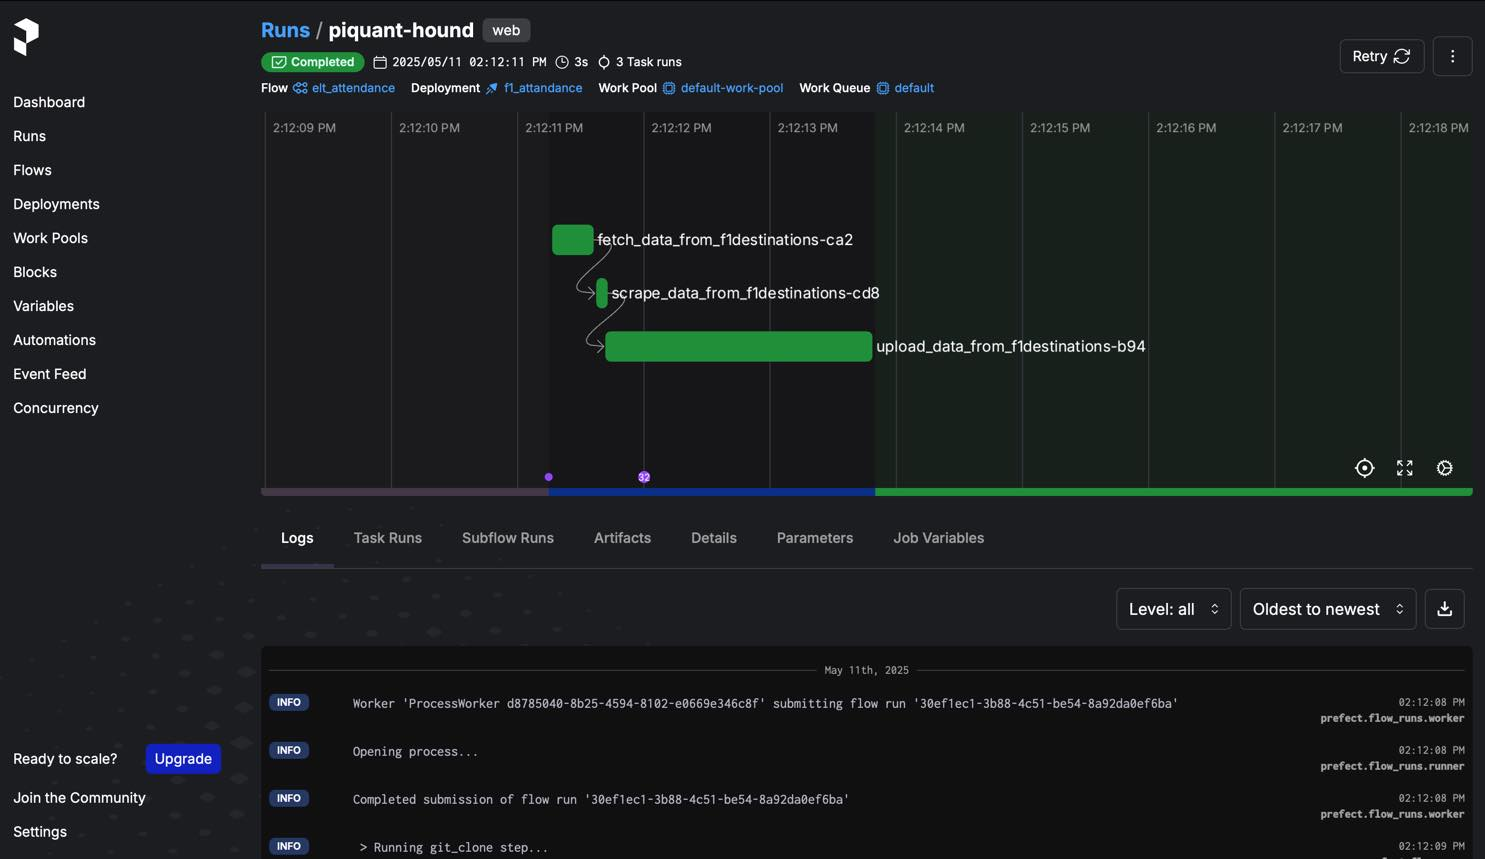
\includegraphics[width=\textwidth]{sc1.jpg}
    \caption{Proces zbierania danych dotyczących liczby osób na poszczególnych wyścigach}
\end{figure}

\begin{figure}[H]
    \centering
    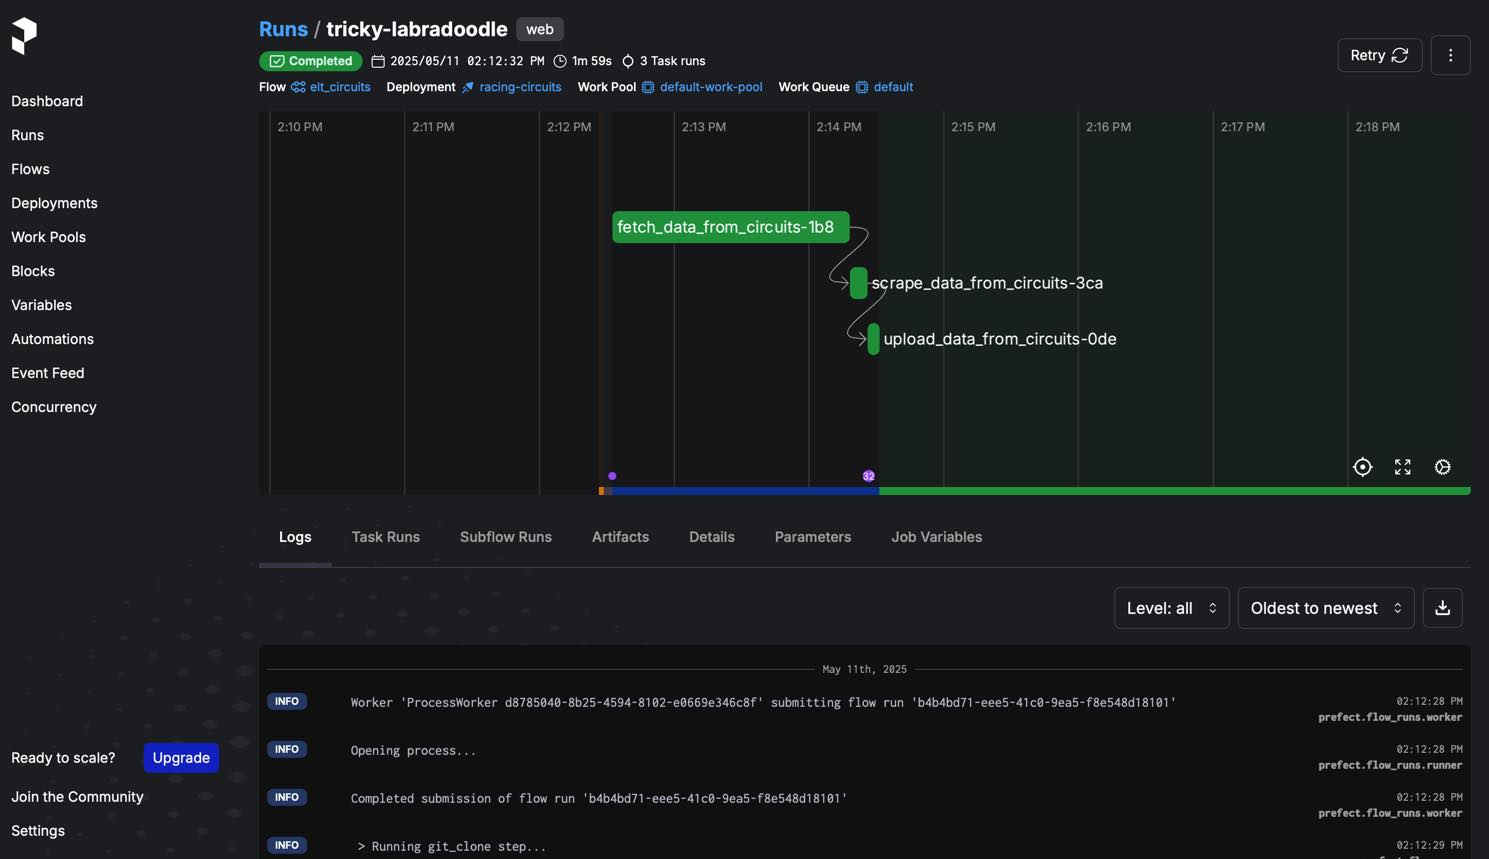
\includegraphics[width=\textwidth]{sc2.jpg}
    \caption{Proces zbierania danych dotyczących torów wyścigowych}
\end{figure}

\begin{figure}[H]
    \centering
    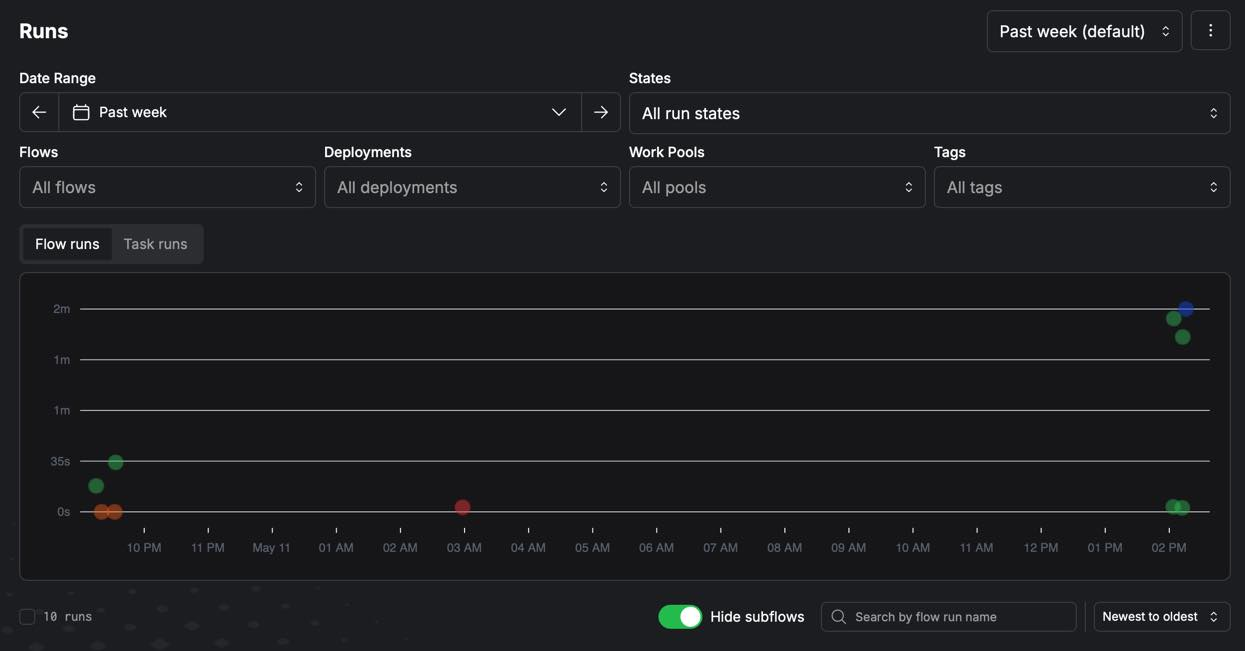
\includegraphics[width=\textwidth]{sc4.jpg}
    \caption{Przeprowadzone procesy}
\end{figure}

\begin{figure}[H]
    \centering
    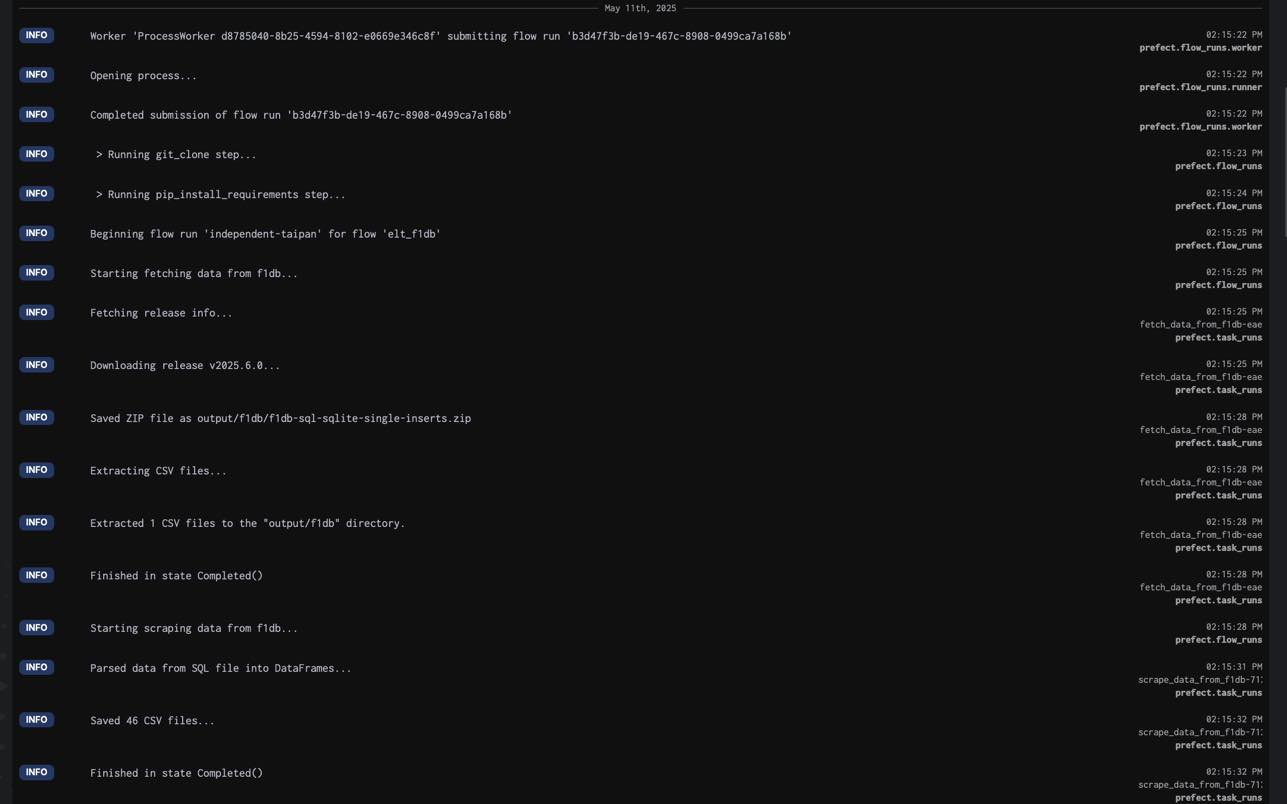
\includegraphics[width=\textwidth]{sc5.jpg}
    \caption{Przykład logów podczas ładowania danych}


\end{figure}

\subsection{Test ponownego wczytywania danych do bazy danych.}
W przypadku ponownego włączenia procesu ładującego dane do bazy w celu uaktualnienia danych po ostatnich wyścigach widzimy, że zostały dodane tylko ostanie rekordy związane z ostatnim wyścigiem.

\begin{itemize}
    \item \textit{Cel:} Testowanie poprawności aktualizacji danych w bazie F1
    \item \textit{Sposób:}
    Testy są wykonane za pomocą sprawdzenia logów z Prefecta oraz wyświetleniu liczby wierszy przed wczytaniem danych oraz po wczytaniu i sprawdzenia.
     \item \textit{Oczekiwany wynik:}
     Liczba wierszy wczytanych w logu powinna być zgodna z liczbą wierszy po aktualizacji, liczba wierszy modyfikowanych plus wierszy przed aktualizacją jest równa liczbie wierszy po aktualizacji.
      \item \textit{Potwierdzenie:}
\end{itemize}

\begin{figure}[H]
    \centering   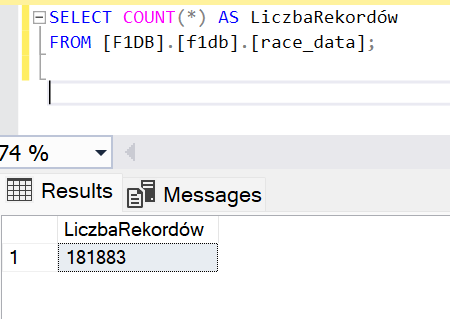
\includegraphics[width=0.6\textwidth]{test2.png}
    \caption{Liczba wierszy w tabeli race\_data po pierwszym załadowaniu danych}
\end{figure}

\begin{figure}[H]
    \centering   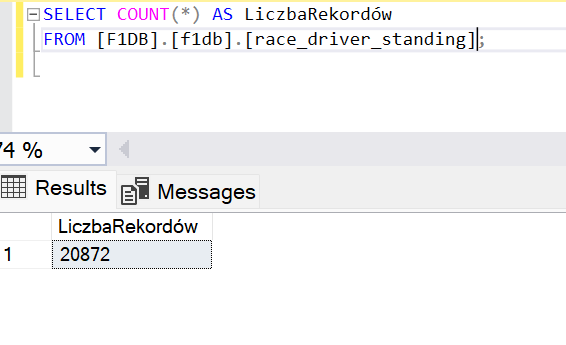
\includegraphics[width=0.6\textwidth]{test3.png}
    \caption{Liczba wierszy w tabeli race\_driver\_standing po pierwszym załadowaniu danych}
\end{figure}

Ładujemy dane po ostatnim wyścigu. Poniżej widzimy procedurę ładowania oraz wyniki po aktualizacji dla tych 2 tabel:

\begin{figure}[H]
    \centering   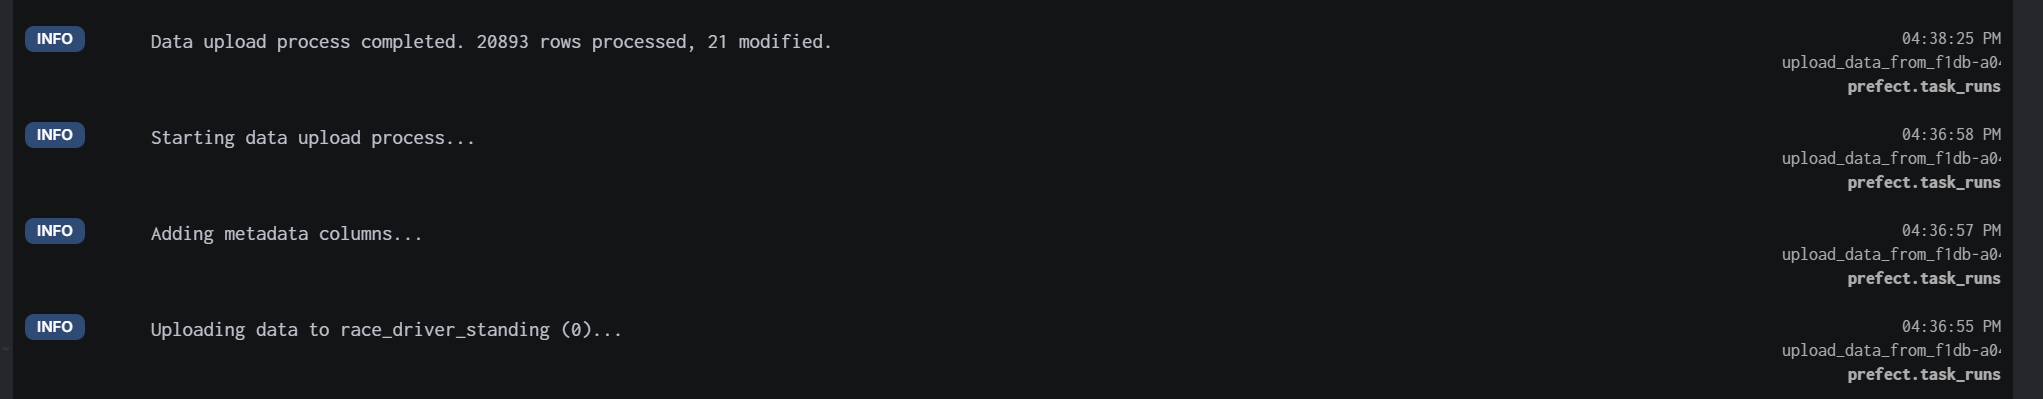
\includegraphics[width=\textwidth]{test4.png}
    \caption{Pokaz logów z ładownia danych dla tabeli race\_driver\_standing}
\end{figure}
Widzimy, że zostało załadowane 20893 z czego 21 zmodyfikowanych oznaczających zmianę rankingu po wyścigu co by się zgadzało.
\begin{figure}[H]
    \centering   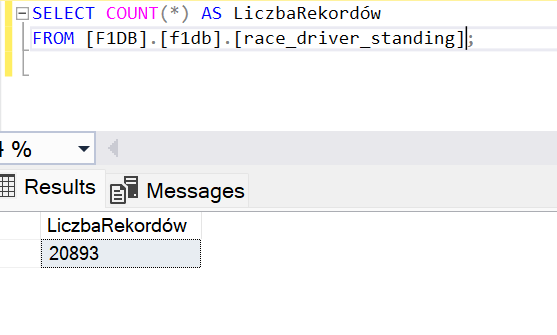
\includegraphics[width=0.6\textwidth]{test5.png}
    \caption{Liczba wierszy w tabeli race\_driver\_standing po aktualizacji z ostatniego wyścigu}
\end{figure}
Widzimy że liczba wierszy się zgadza. Poniżej sprawdzamy czy dane dla \textit{race\_data} też załadowały się poprawnie.

\begin{figure}[H]
    \centering   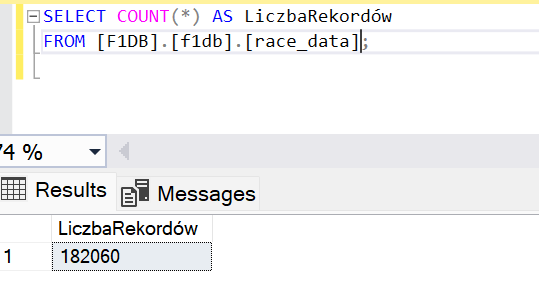
\includegraphics[width=0.6\textwidth]{test6.png}
    \caption{Liczba wierszy w tabeli race\_data po aktualizacji z ostatniego wyścigu}
\end{figure}
Widzimy, że dane zostały faktycznie dodane.

\subsection{Test ponownego wczytywania danych do bazy danych scrapowanych ze strony z oglądalnością wyścigów oraz ze strony z informacjami torów.}
Testy przebiegają identycznie co w przypadku powyżej.

\begin{itemize}
    \item \textit{Cel:} Testowanie poprawności aktualizacji danych w bazie F1 ze scrapowanych stron.
    \item \textit{Sposób:}
    Testy są wykonane za pomocą sprawdzenia logów z Prefecta oraz wyświetleniu liczby wierszy przed wczytaniem danych oraz po wczytaniu i sprawdzenia.
     \item \textit{Oczekiwany wynik:}
     Liczba wierszy wczytanych w logu powinna być zgodna z liczbą wierszy po aktualizacji oraz z liczbą wiersz przed, ponieważ strona z wynikiem oglądalności nie została zaktualizowana.
      \item \textit{Potwierdzenie:}
\end{itemize}

\begin{figure}[H]
    \centering   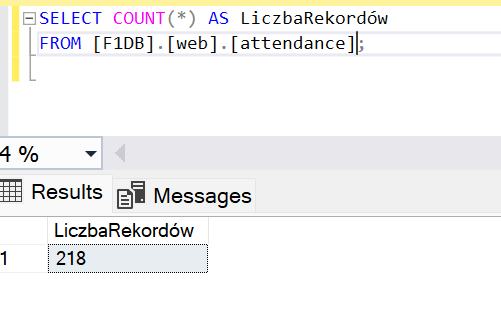
\includegraphics[width=0.6\textwidth]{test7.png}
    \caption{Liczba wierszy w tabeli web\_attendence przed aktualizacją}
\end{figure}


\begin{figure}[H]
    \centering   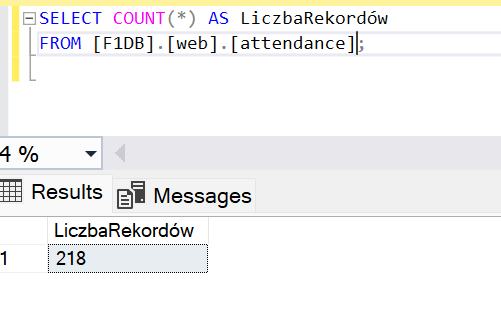
\includegraphics[width=0.6\textwidth]{test7.png}
    \caption{Liczba wierszy w tabeli web\_attendence po aktualizacji}
\end{figure}

\begin{figure}[H]
    \centering   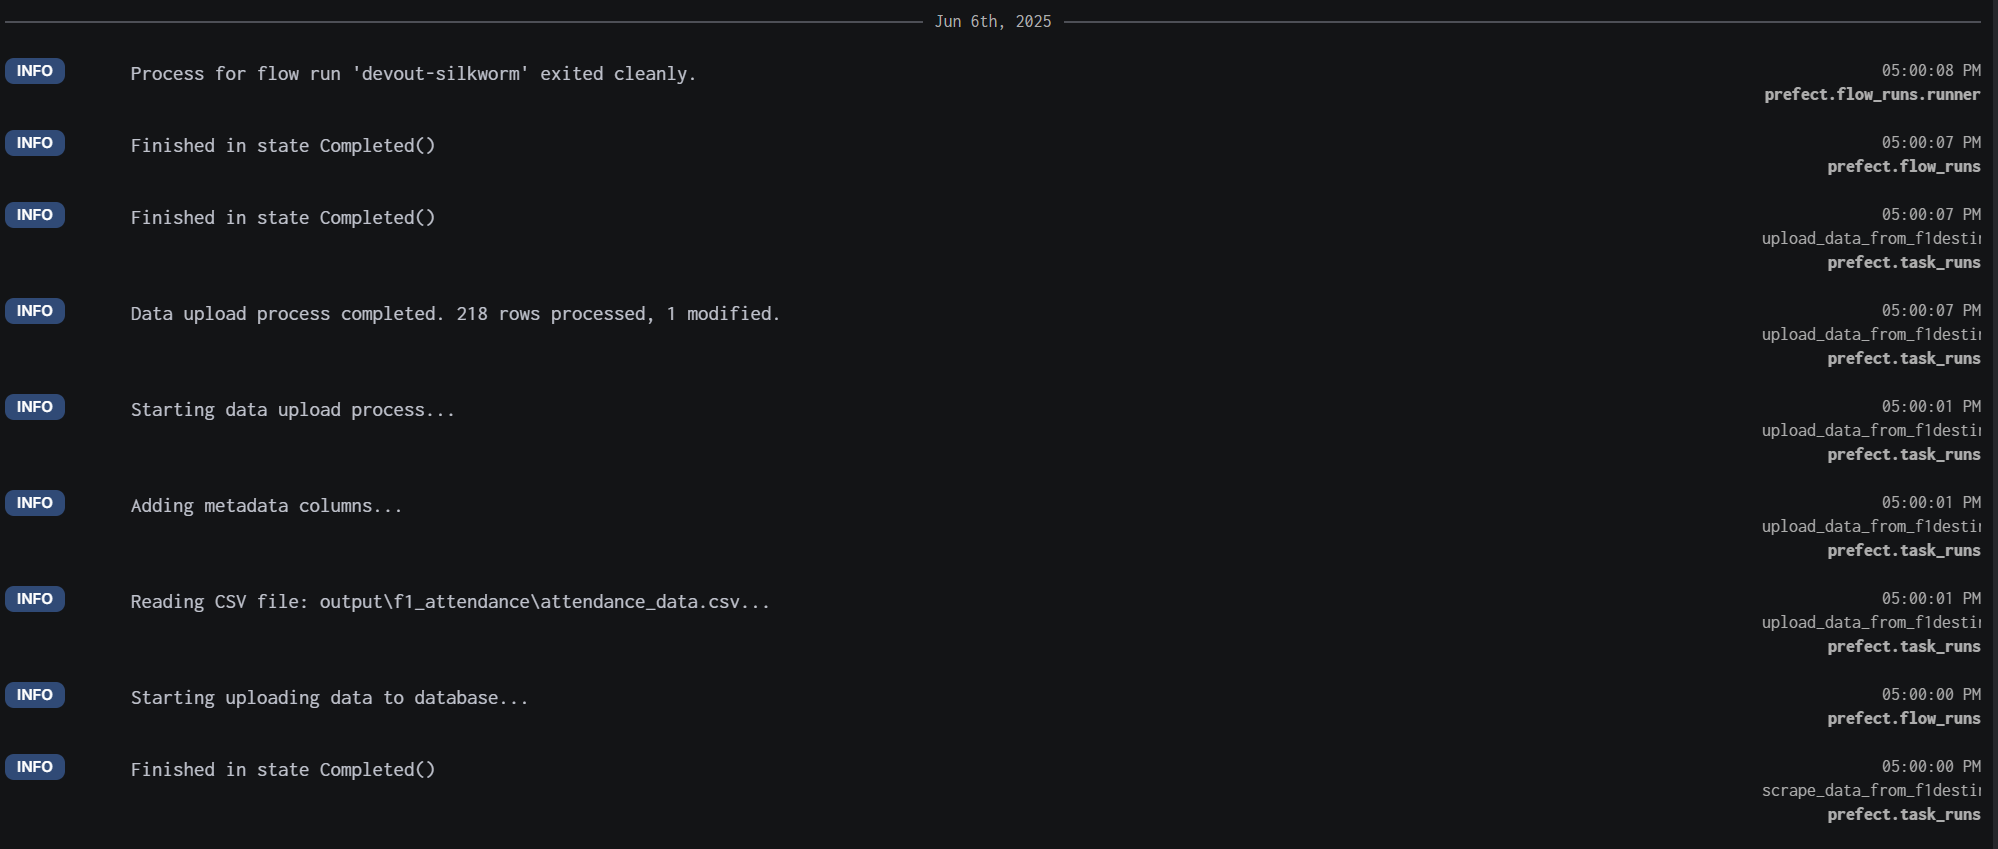
\includegraphics[width=\textwidth]{test8.png}
    \caption{Logi z Prefecta podczas aktualizacji}
\end{figure}

W przypadku \textit{circuit\_details} robimy to samo:

\begin{figure}[H]
    \centering   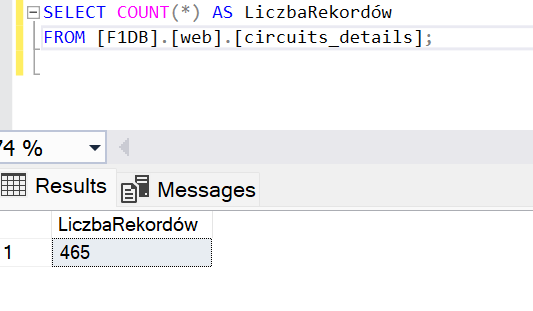
\includegraphics[width=0.6\textwidth]{test9.png}
    \caption{Liczba wierszy w tabeli web\_circuit\_details przed aktualizacją}
\end{figure}


\begin{figure}[H]
    \centering   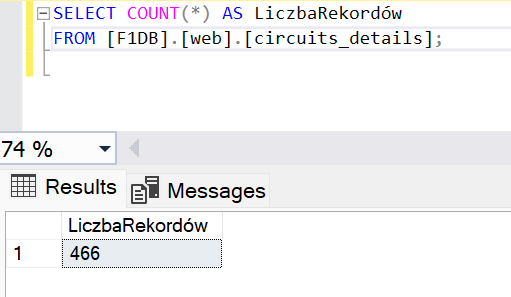
\includegraphics[width=0.6\textwidth]{test11.png}
    \caption{Liczba wierszy w tabeli web\_circuit\_details po aktualizacji}
\end{figure}

\begin{figure}[H]
    \centering   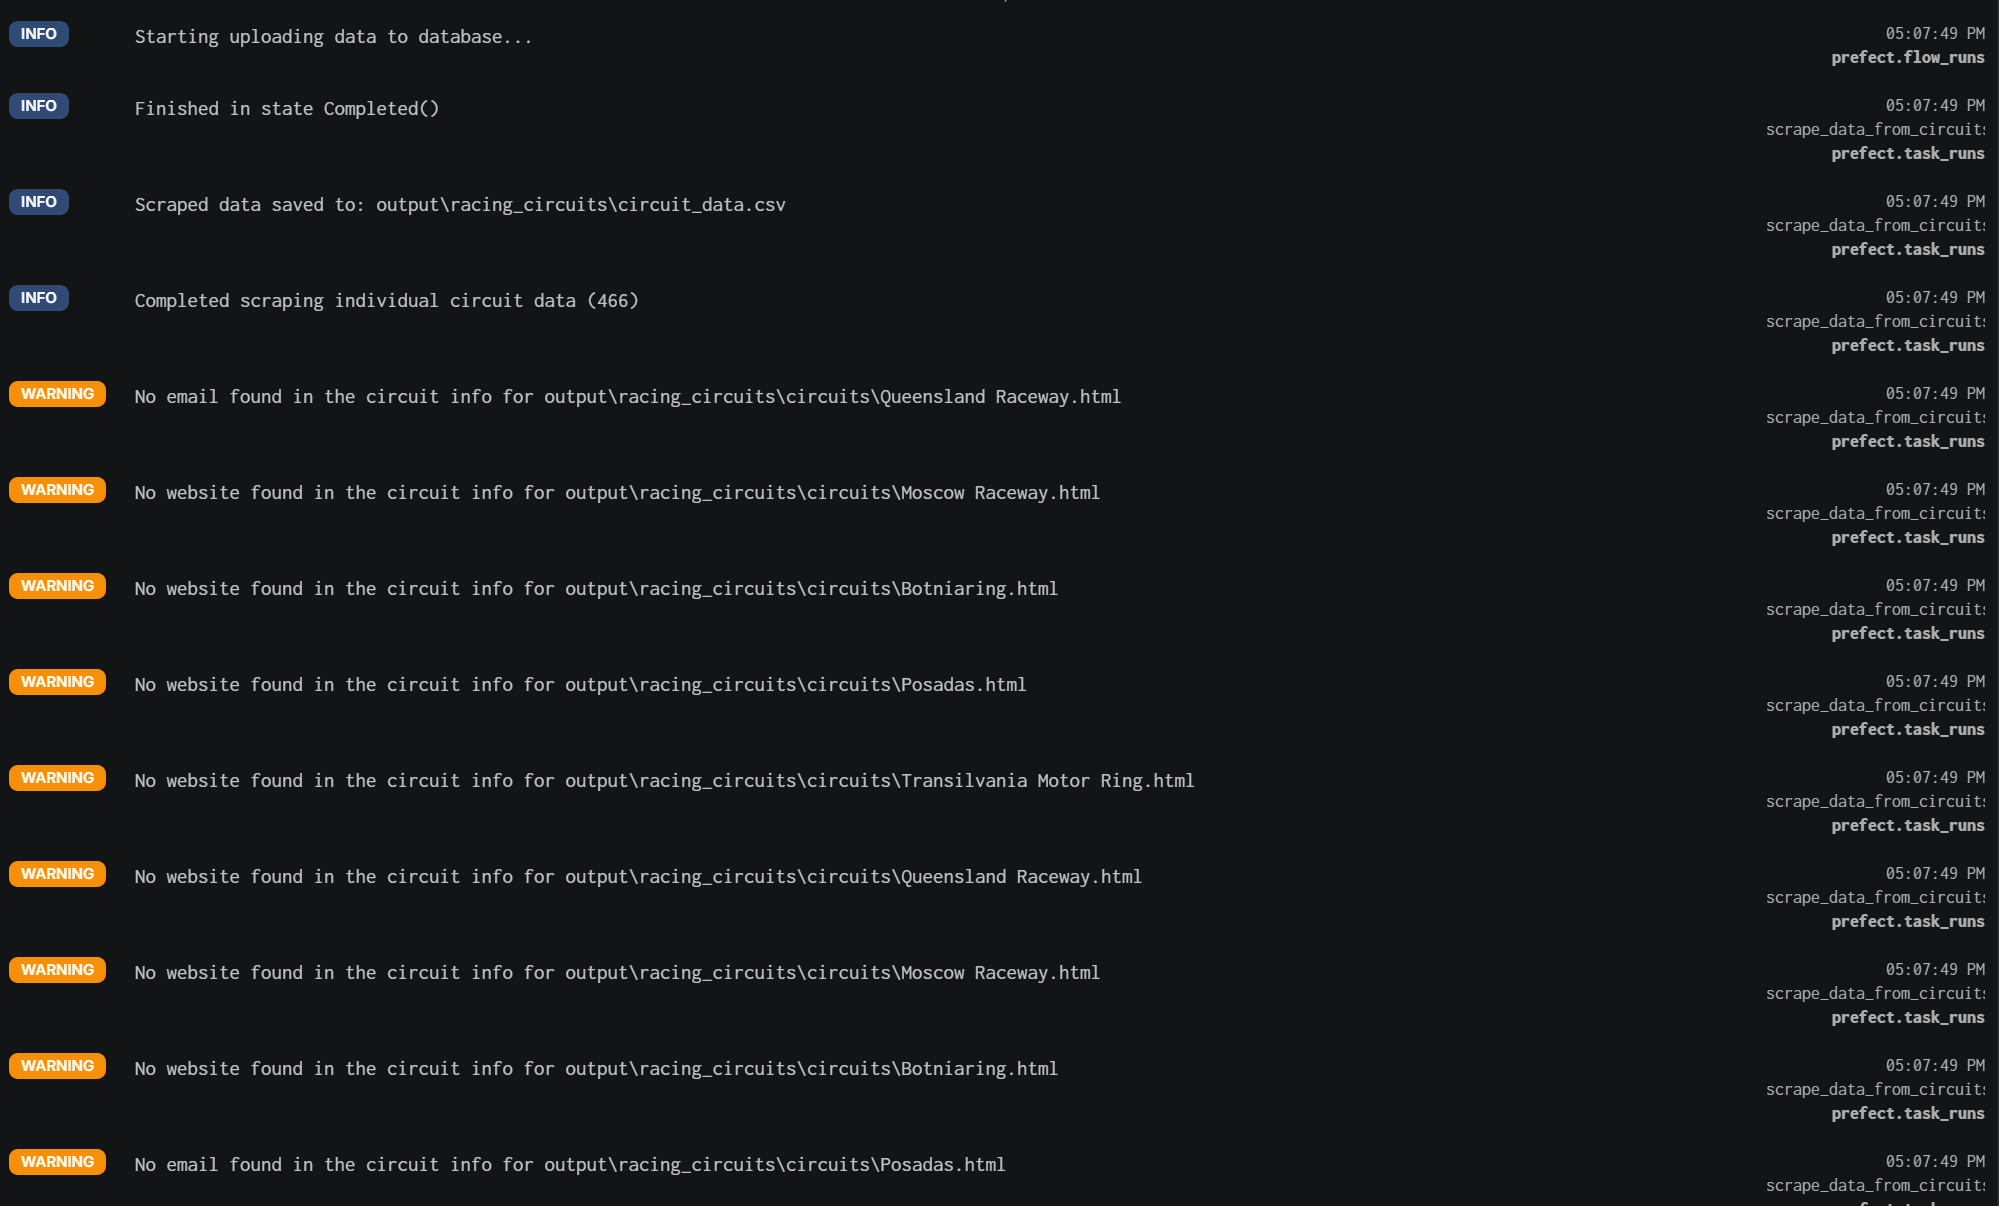
\includegraphics[width=\textwidth]{test10.png}
    \caption{Logi z Prefecta podczas aktualizacji}
\end{figure}
W logach widzimy ostrzeżenia, że w przypadku niektórych torów informacje na stronie są niekompletne. Widzimy, że liczba wiersz z logów zgadza się z tym co jest po w SQL, został dodany jeden nowy tor.

\subsection{Test ponownego procesu ETL z bazy do hurtowni danych.}
\begin{itemize}
    \item \textit{Cel:} Testowanie poprawności aktualizacji danych w hurtowni F1 po procesie ETL.
    \item \textit{Sposób:}
    Testy są wykonane za pomocą sprawdzenia logów z Prefecta oraz wyświetleniu liczby wierszy przed wczytaniem danych oraz po wczytaniu i sprawdzenia.
     \item \textit{Oczekiwany wynik:}
     Liczba nowych wierszy w logu plus liczba wiersz w hurtowni przed aktualizacją powinna być równa liczbie wierszy po aktualizacji.
      \item \textit{Potwierdzenie:}
\end{itemize}
\begin{figure}[H]
    \centering   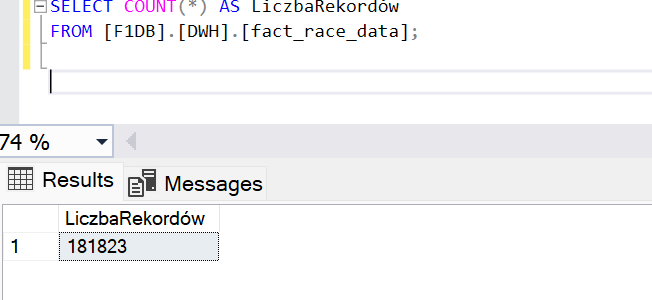
\includegraphics[width=0.6\textwidth]{test12.png}
    \caption{Liczba wierszy w tabeli DW\_fact\_race\_data przed aktualizacją}
\end{figure}


\begin{figure}[H]
    \centering   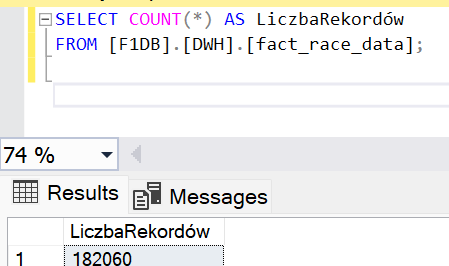
\includegraphics[width=0.6\textwidth]{test14.png}
    \caption{Liczba wierszy w tabeli DW\_fact\_race\_data po aktualizacją}
\end{figure}

\begin{figure}[H]
    \centering   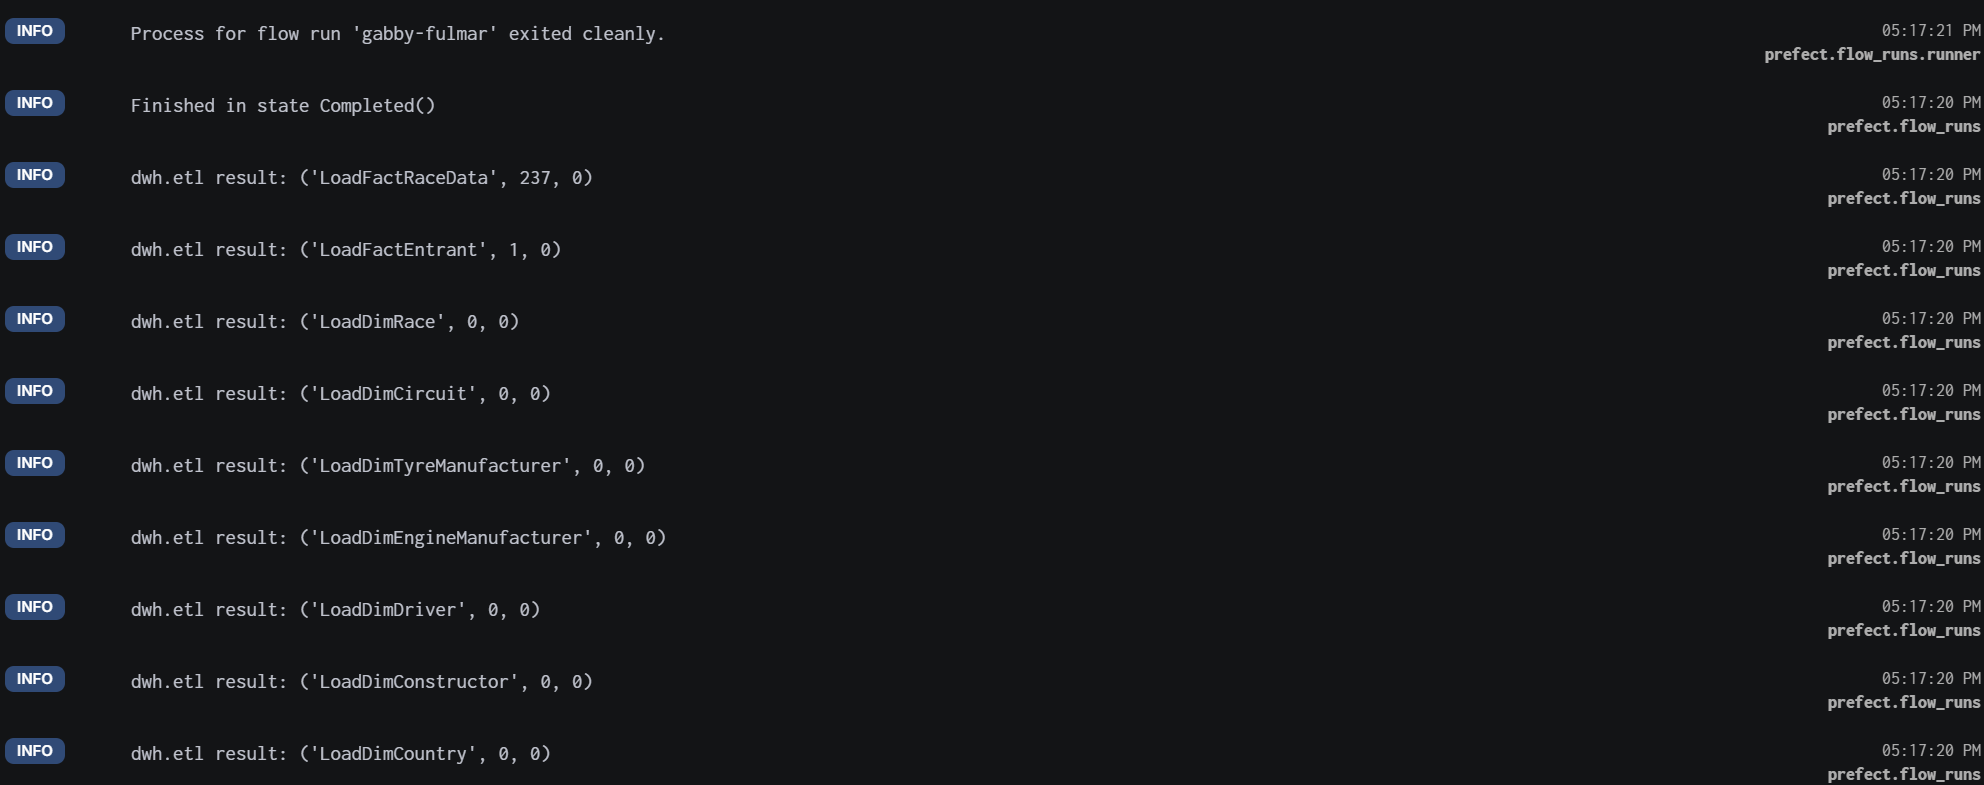
\includegraphics[width=\textwidth]{test13.png}
    \caption{Logi z Prefecta podczas aktualizacji}
\end{figure}

Jaki widać po zsumowaniu wszystko się zgadza. Widzimy też że zostały dodane wiersze tylko w tabelach faktowych gdzie znajdują się nowe dane z ostatniego wyścigu.


\subsection{Test zmiany danych, które nie mogą być zmieniane w hurtowni.}
\begin{itemize}
    \item \textit{Cel:} Sprawdzenie czy na pewno nie da się zmienić danych w hurtowni, których nie powinno dać się zmienić
    \item \textit{Sposób:}
   Zmieniamy ręcznie dane, których nie powinno dać się zmienić, przeprowadzamy proces ETL i sprawdzamy czy się zmodyfikowały.
     \item \textit{Oczekiwany wynik:}
     Testowany wiersz nie uległ zmianie, wyrzuca błąd, że nie da się go zmienić
      \item \textit{Potwierdzenie:}
\end{itemize}

\begin{figure}[H]
    \centering   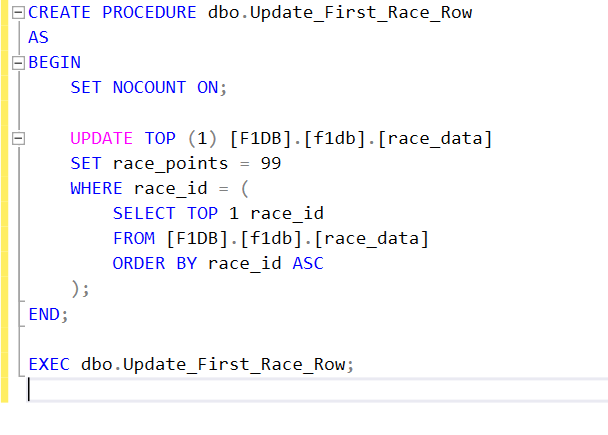
\includegraphics[width=0.6\textwidth]{test16.png}
    \caption{Testowa kwerenda zmieniając wiersz}
\end{figure}

\begin{figure}[H]
    \centering   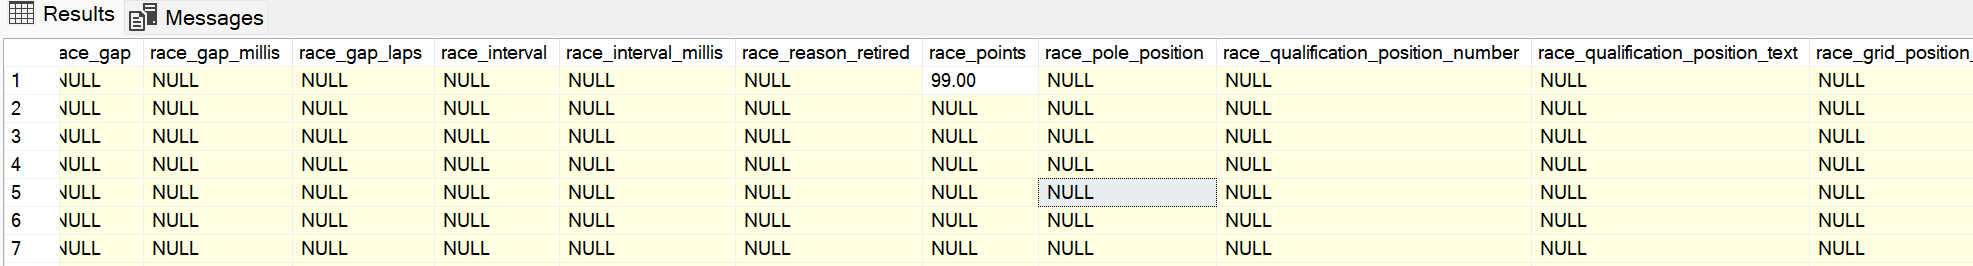
\includegraphics[width=\textwidth]{test15.png}
    \caption{Rezultat kwerendy}
\end{figure}

\begin{figure}[H]
    \centering   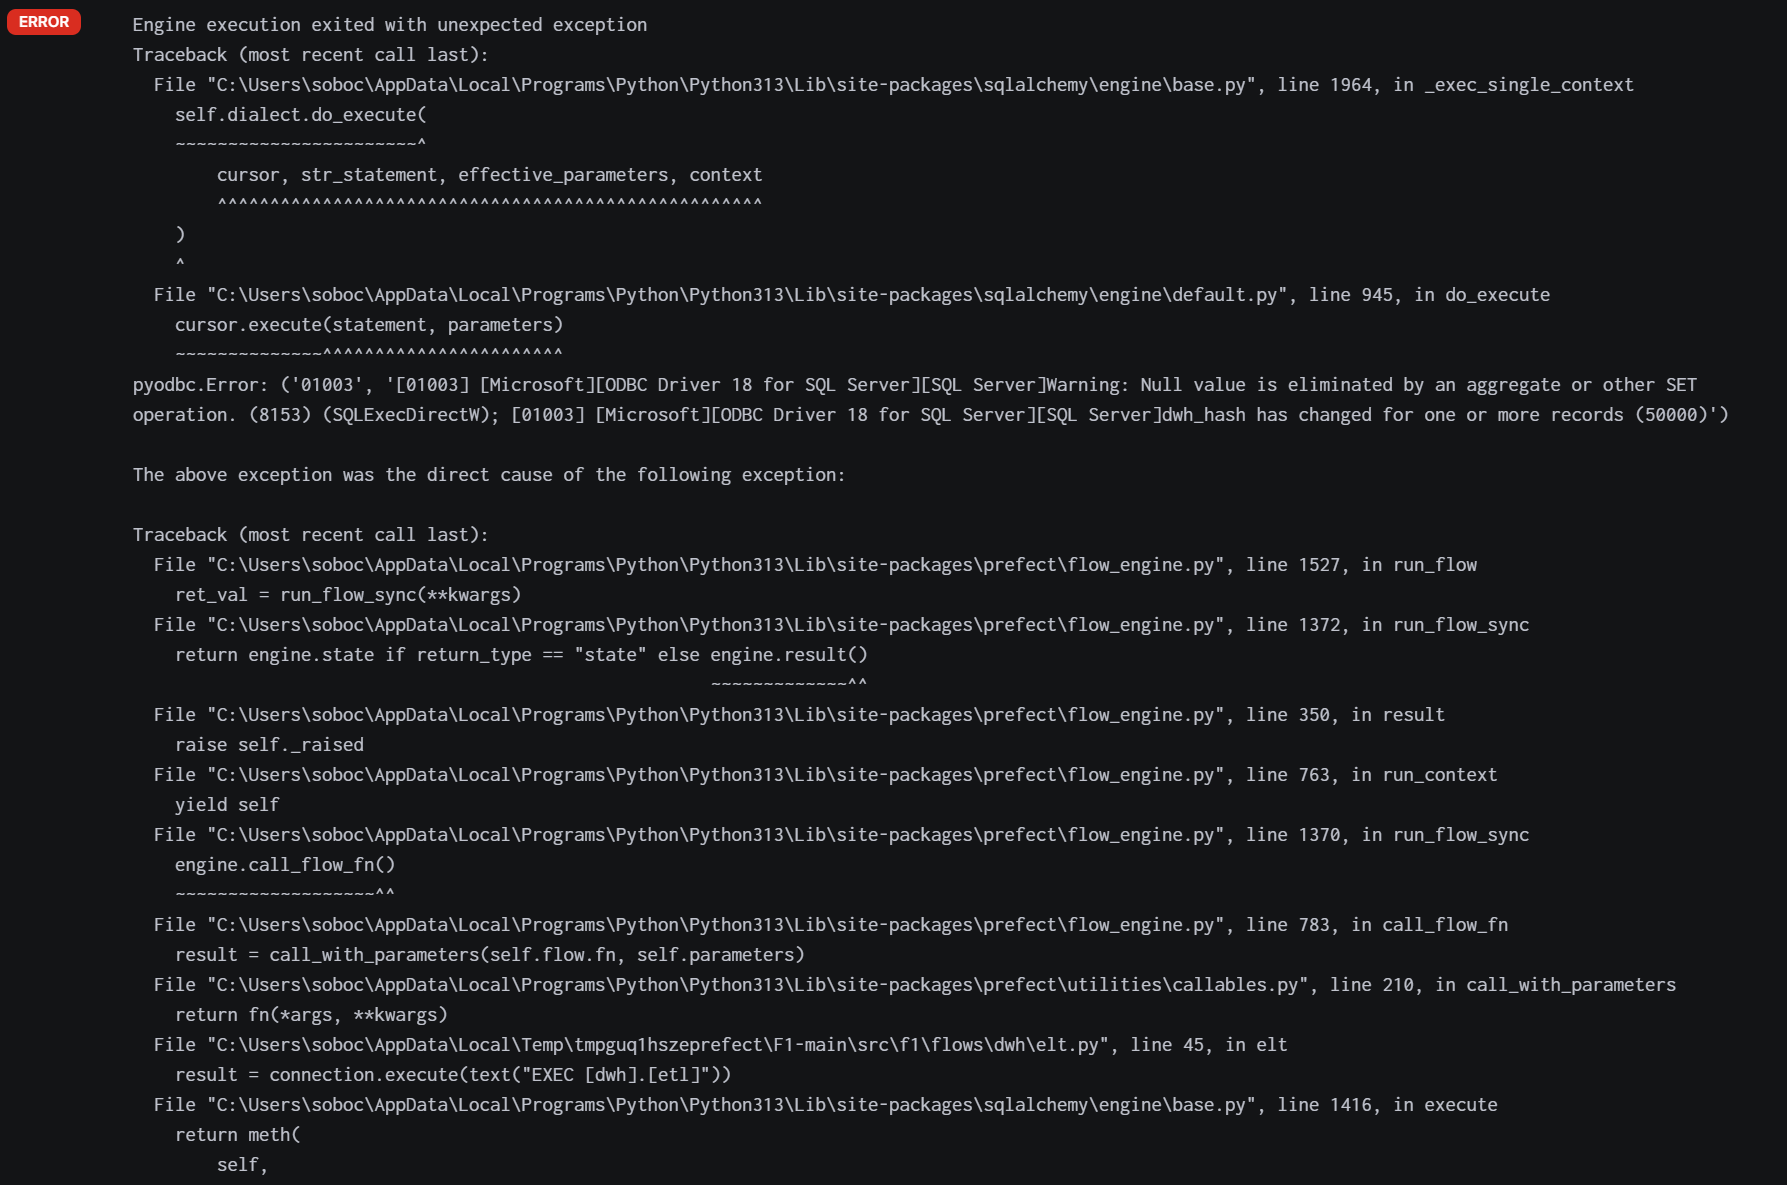
\includegraphics[width=\textwidth]{test22.png}
    \caption{Logi z prefecta. Wyskakuj błąd, że nie da się zmienić tego wiersza.}
\end{figure}


\subsection{Test zmiany danych, które mogą być zmieniane w hurtowni.}
\begin{itemize}
    \item \textit{Cel:} Sprawdzenie czy da się zmienić dane w hurtowni, które mogą być zmienione.
    \item \textit{Sposób:}
   Zmieniamy ręcznie dane, których mogą być zmienione, przeprowadzamy proces ETL i sprawdzamy czy się zmodyfikowały.
     \item \textit{Oczekiwany wynik:}
     Testowany wiersz uległ zmianie.
      \item \textit{Potwierdzenie:}
\end{itemize}

\begin{figure}[H]
    \centering   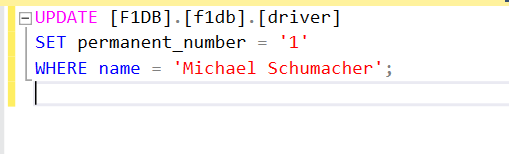
\includegraphics[width=0.6\textwidth]{test18.png}
    \caption{Testowa kwerenda zmieniając wiersz}
\end{figure}

\begin{figure}[H]
    \centering   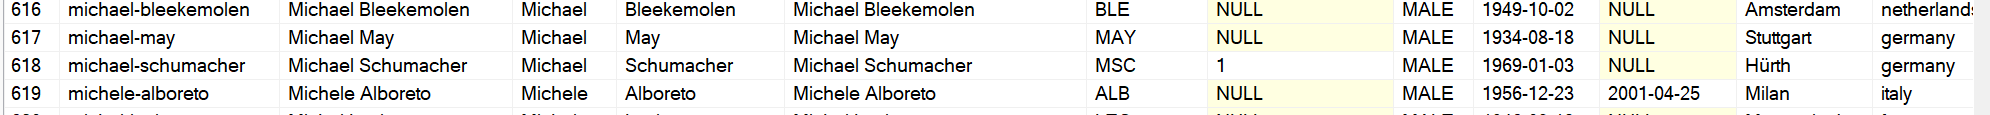
\includegraphics[width=\textwidth]{test17.png}
    \caption{Rezultat kwerendy}
\end{figure}

\begin{figure}[H]
    \centering   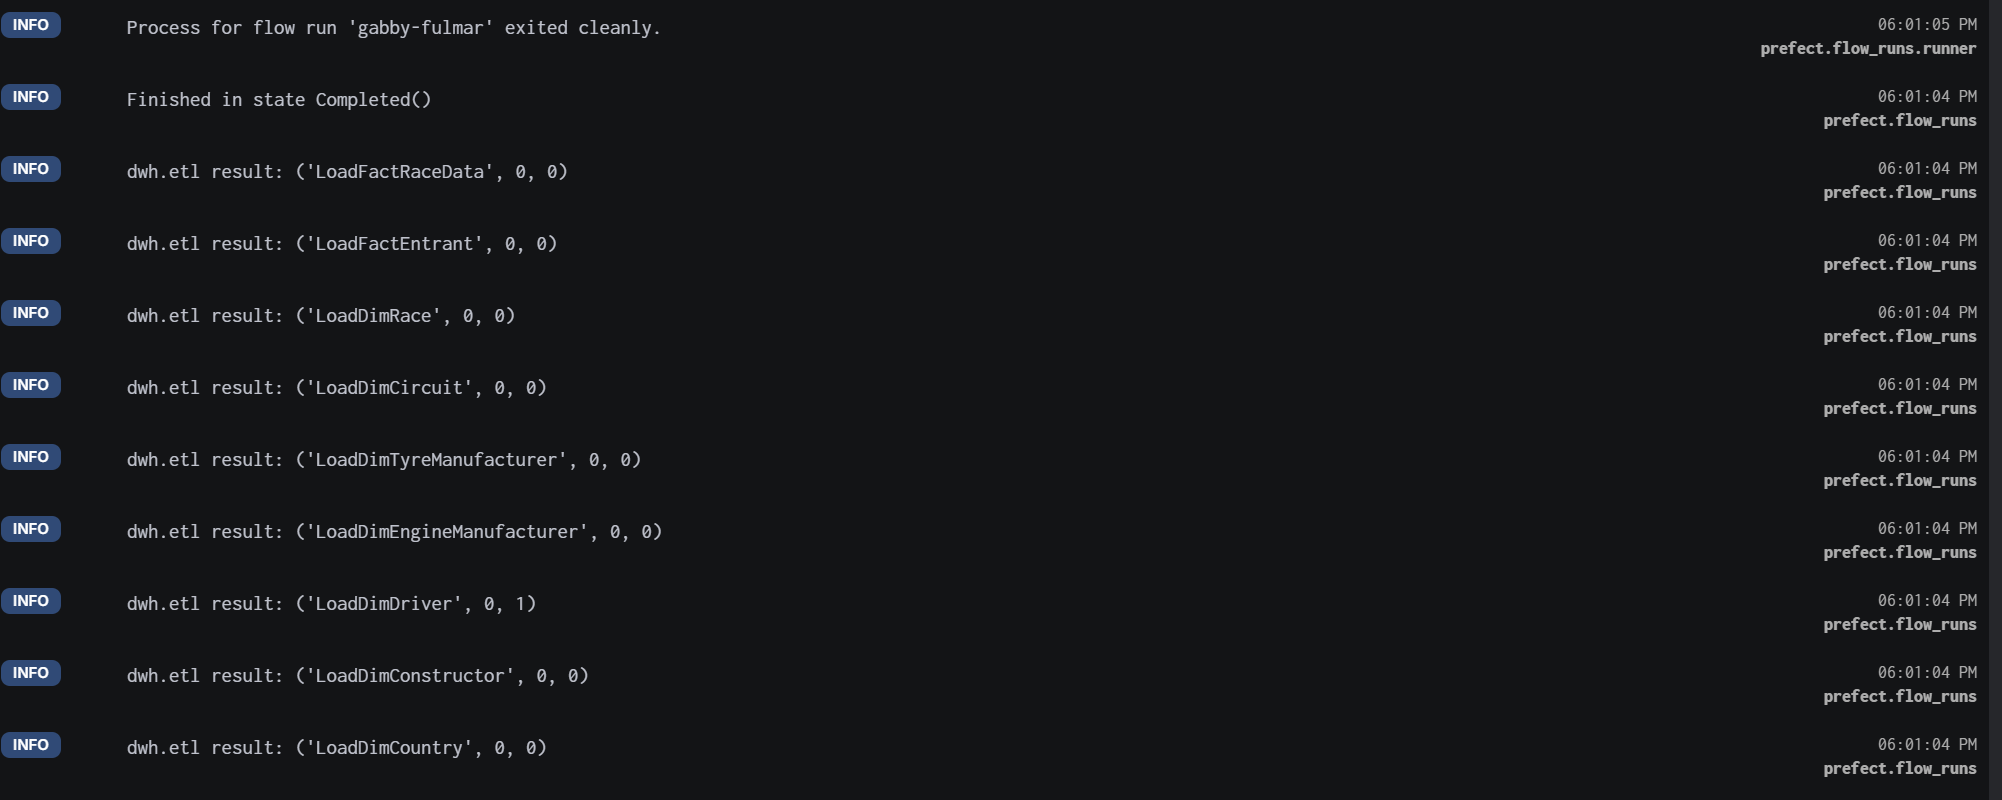
\includegraphics[width=\textwidth]{test20.png}
    \caption{Logi z prefecta pokazujące 1 modyfikację w dim\_driver}
\end{figure}

\begin{figure}[H]
    \centering   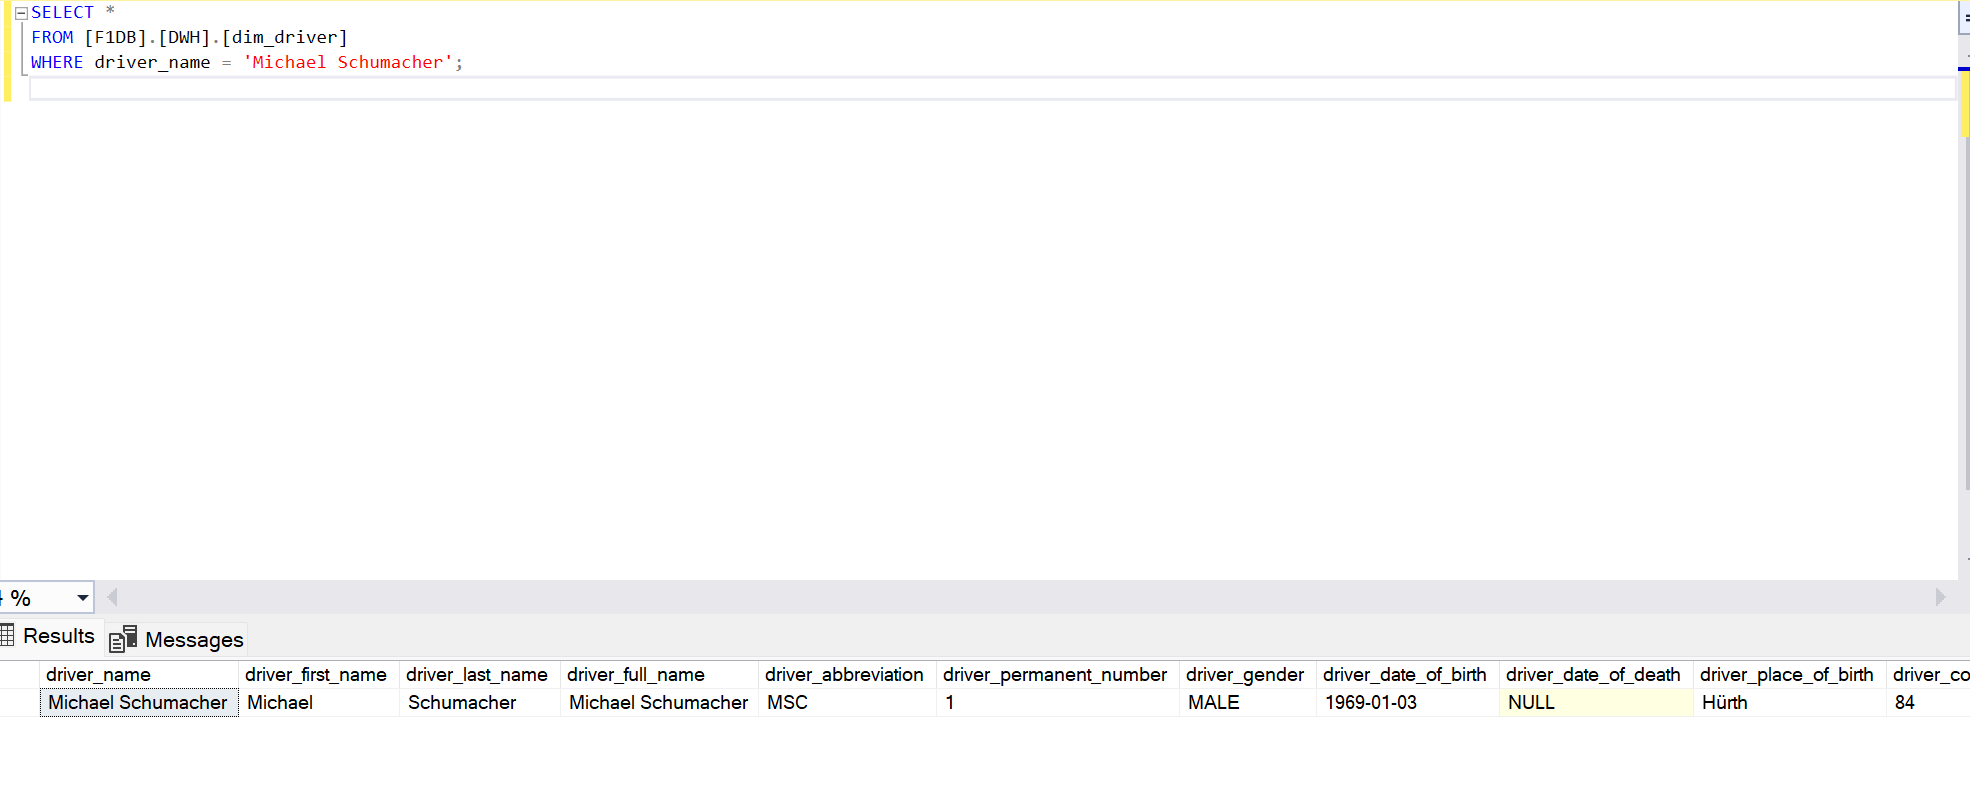
\includegraphics[width=\textwidth]{test21.png}
    \caption{Wynik po modyfikacji}
\end{figure}

\subsection{Testy warstwy raportowej}
\subsubsection*{1 strona raportu}
\begin{itemize}
    \item \textit{Cel:} Test czy dane na wykresach rysują się prawidłowo
    \item \textit{Sposób:}
   Patrzymy co jest na wykresie i wywołamy odpowiednią kwerendę w SQL, żeby potwierdzić zgodność danych
     \item \textit{Oczekiwany wynik:}
     Zarówno w raporcie jak i SQL mamy otrzymać te same wartości.
      \item \textit{Potwierdzenie:}
\end{itemize}

\begin{figure}[H]
    \centering   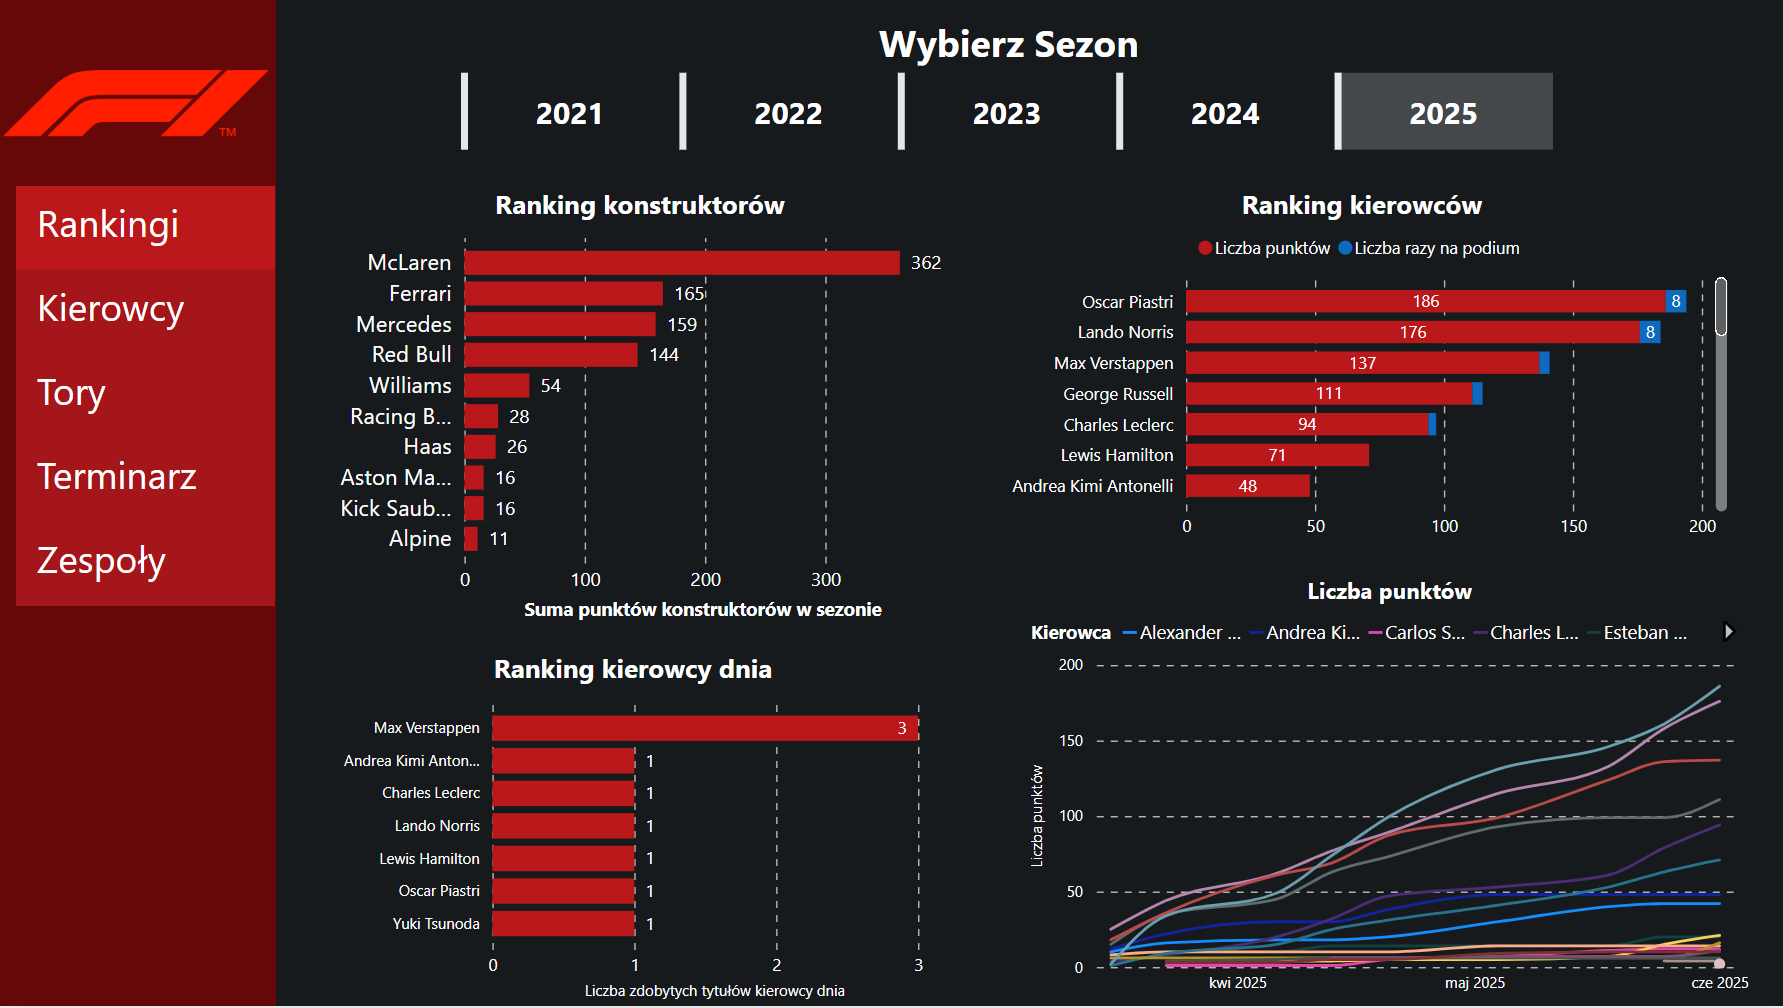
\includegraphics[width=\textwidth]{raport1.png}
    \caption{Testowanie wykresu}
\end{figure}

\begin{figure}[H]
    \centering   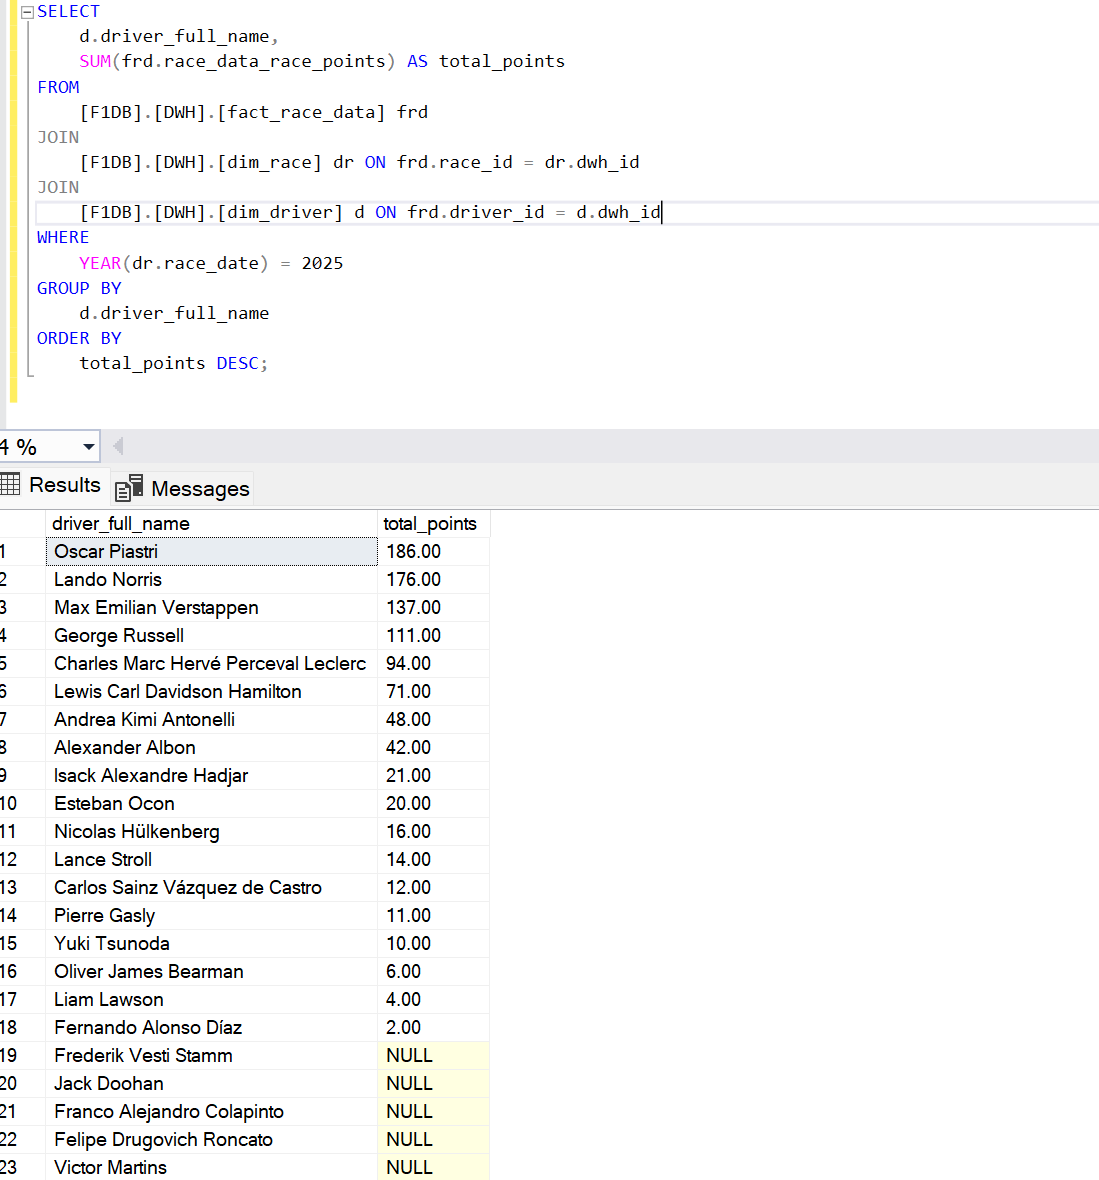
\includegraphics[width=\textwidth]{t1.png}
    \caption{Odpowiednia kwerenda}
\end{figure}

\begin{figure}[H]
    \centering   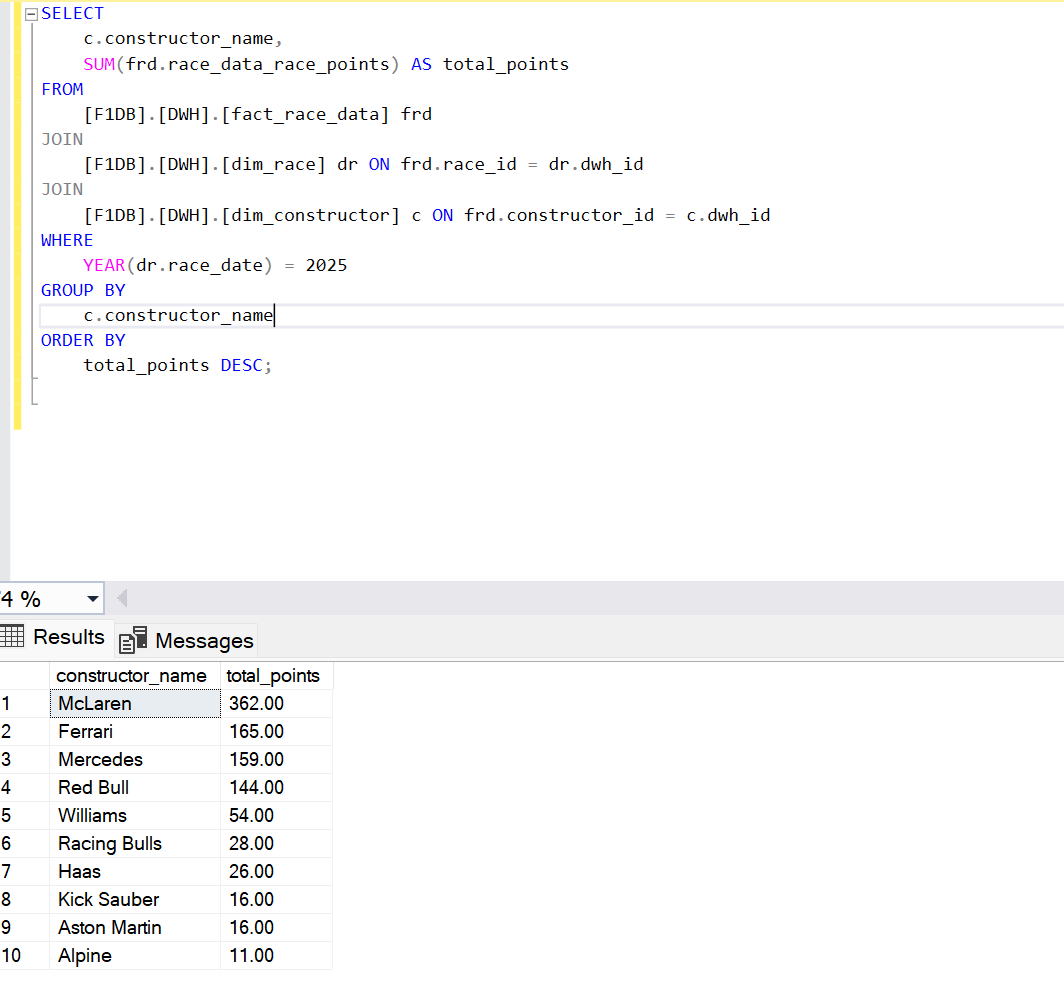
\includegraphics[width=\textwidth]{t2.png}
    \caption{Odpowiednia kwerenda}
\end{figure}

\begin{figure}[H]
    \centering   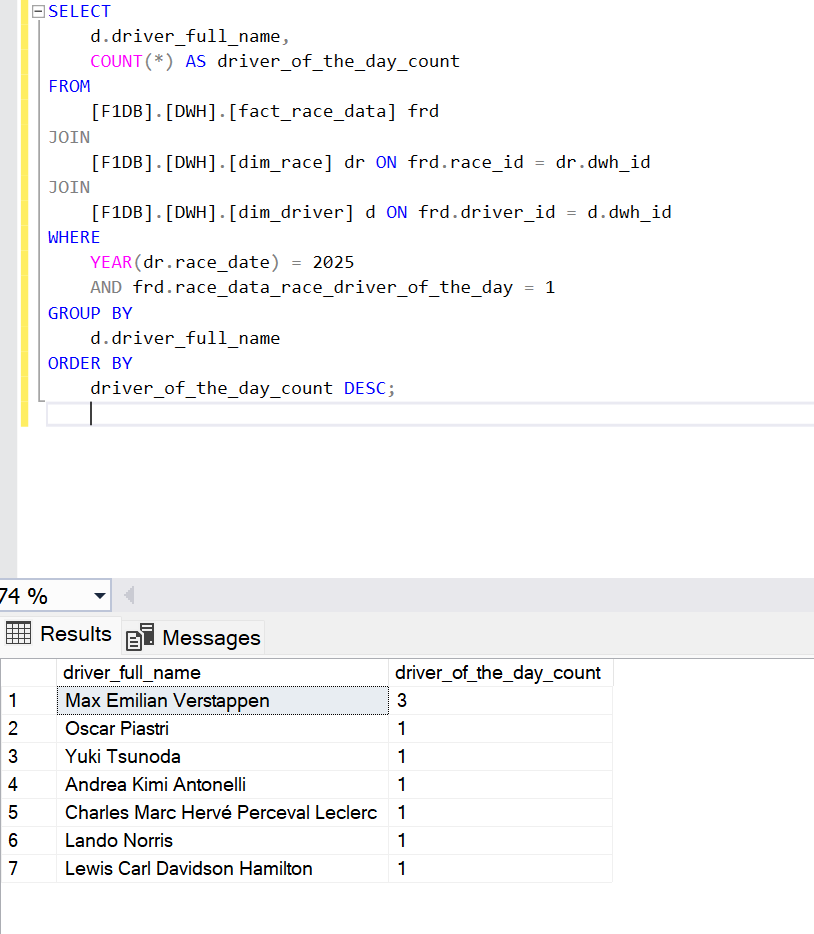
\includegraphics[width=\textwidth]{t3.png}
    \caption{Odpowiednia kwerenda}
\end{figure}

\begin{figure}[H]
    \centering   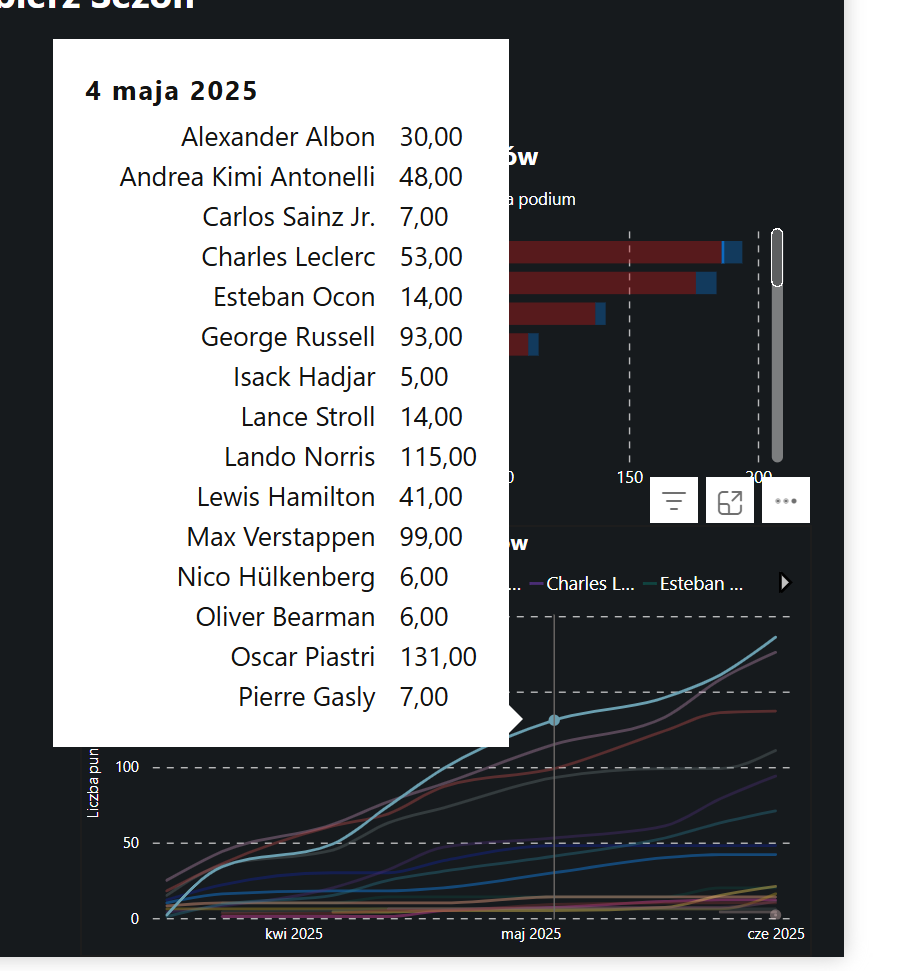
\includegraphics[width=0.6\textwidth]{t4.png}
    \caption{Test wykresu}
\end{figure}

\begin{figure}[H]
    \centering   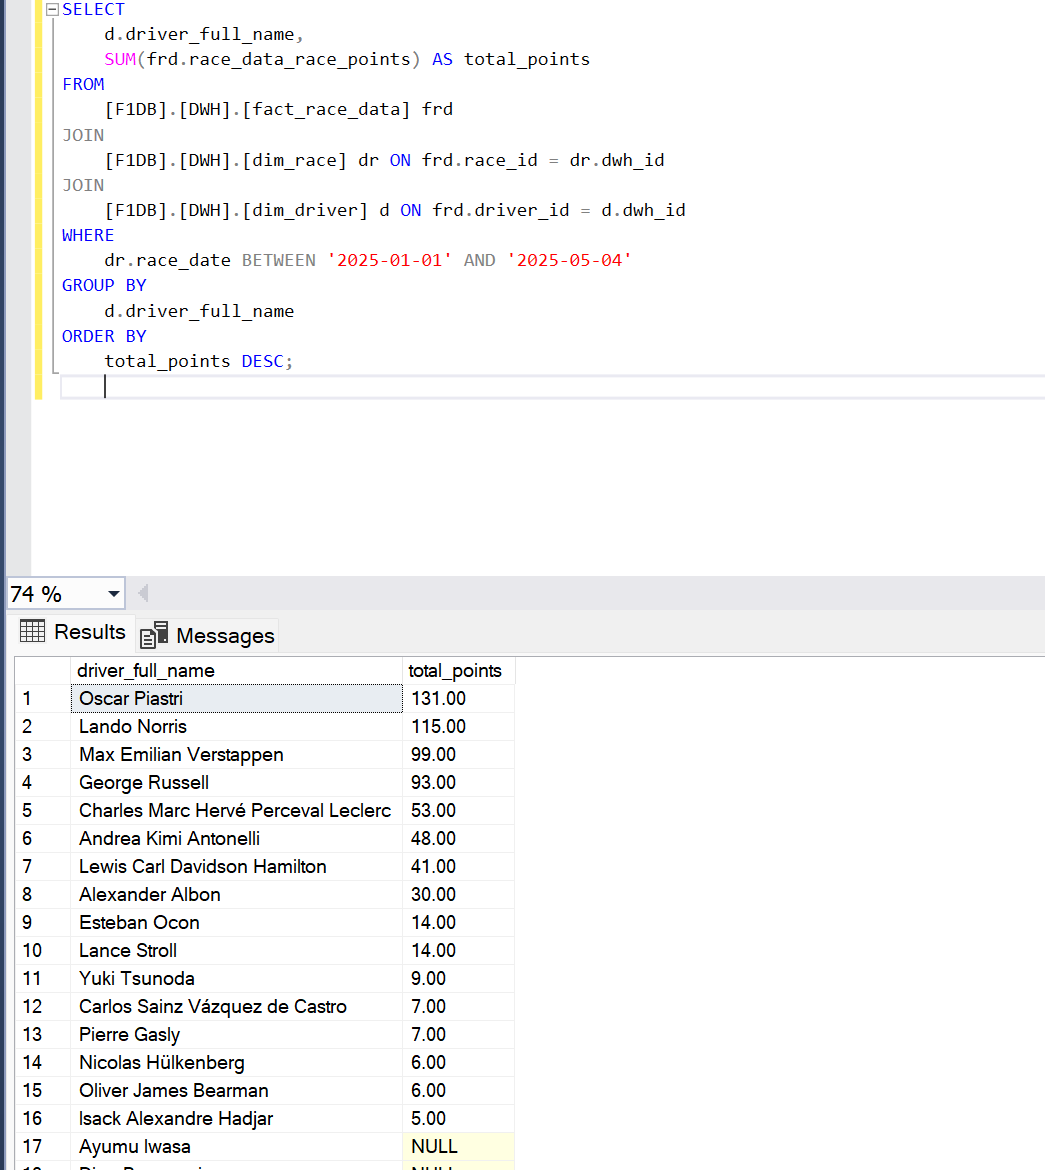
\includegraphics[width=\textwidth]{t5.png}
    \caption{Odpowiednia kwerenda}
\end{figure}

Widzimy, że się wszystko zgadza.

\subsubsection*{2 strona raportu}
Cel i założenia są te same co wyżej.

\begin{figure}[H]
    \centering   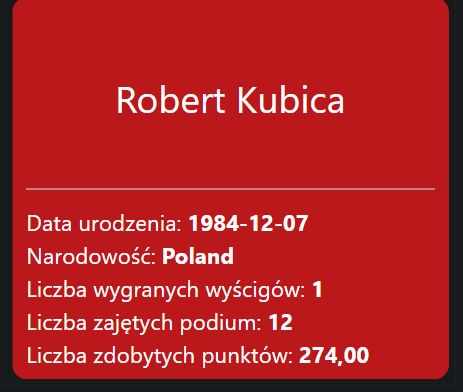
\includegraphics[width=0.4\textwidth]{t6.png}
    \caption{Test wykresu}
\end{figure}

\begin{figure}[H]
    \centering   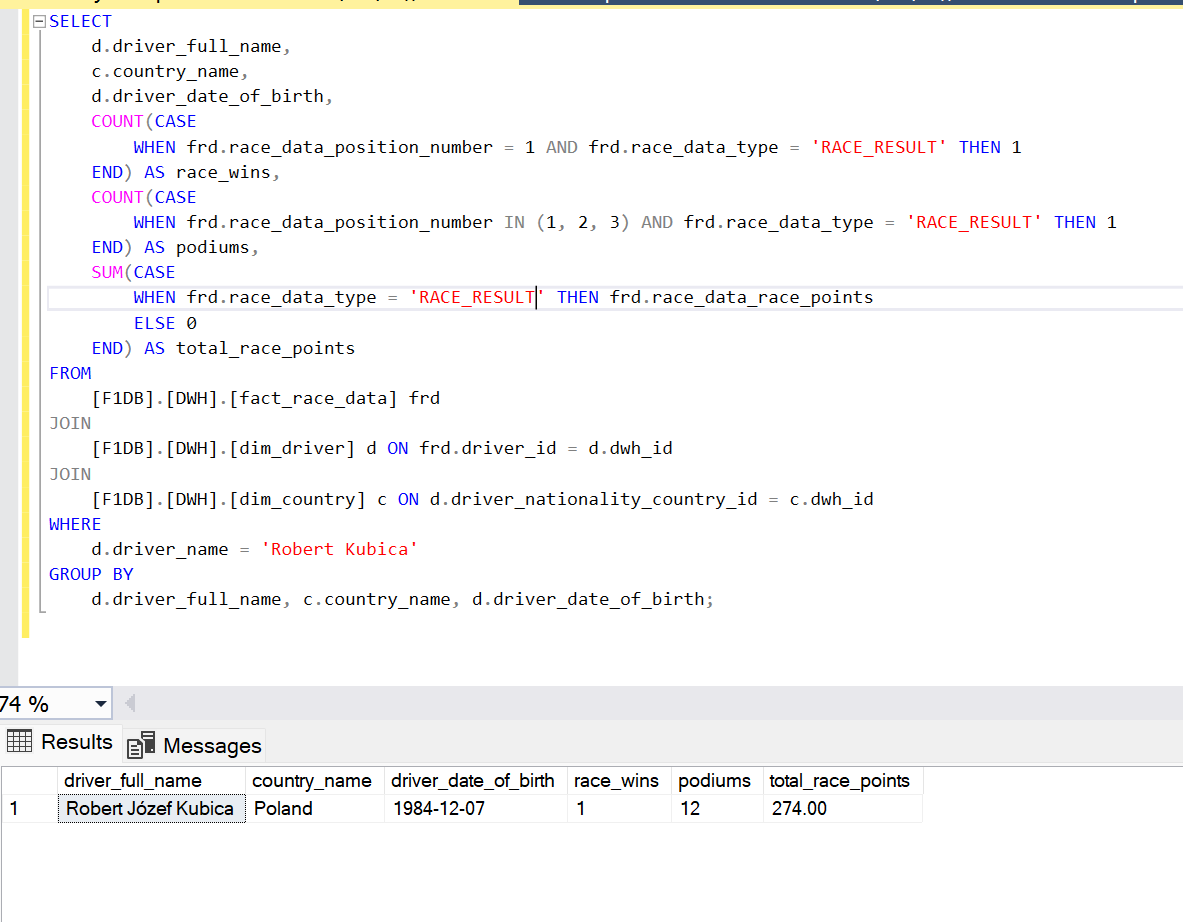
\includegraphics[width=\textwidth]{t7.png}
    \caption{Odpowiednia kwerenda}
\end{figure}

Wszystko zgadza się. Jak wiadomo w czerwcu 2008, podczas Grand Prix Kanady, Robert Kubica odniósł swoje pierwsze i jedyne zwycięstwo w Formule 1, stając się pierwszym Polakiem w historii, który tego dokonał.


\subsubsection*{3 strona raportu}
Cel i założenia są te same co wyżej.

\begin{figure}[H]
    \centering   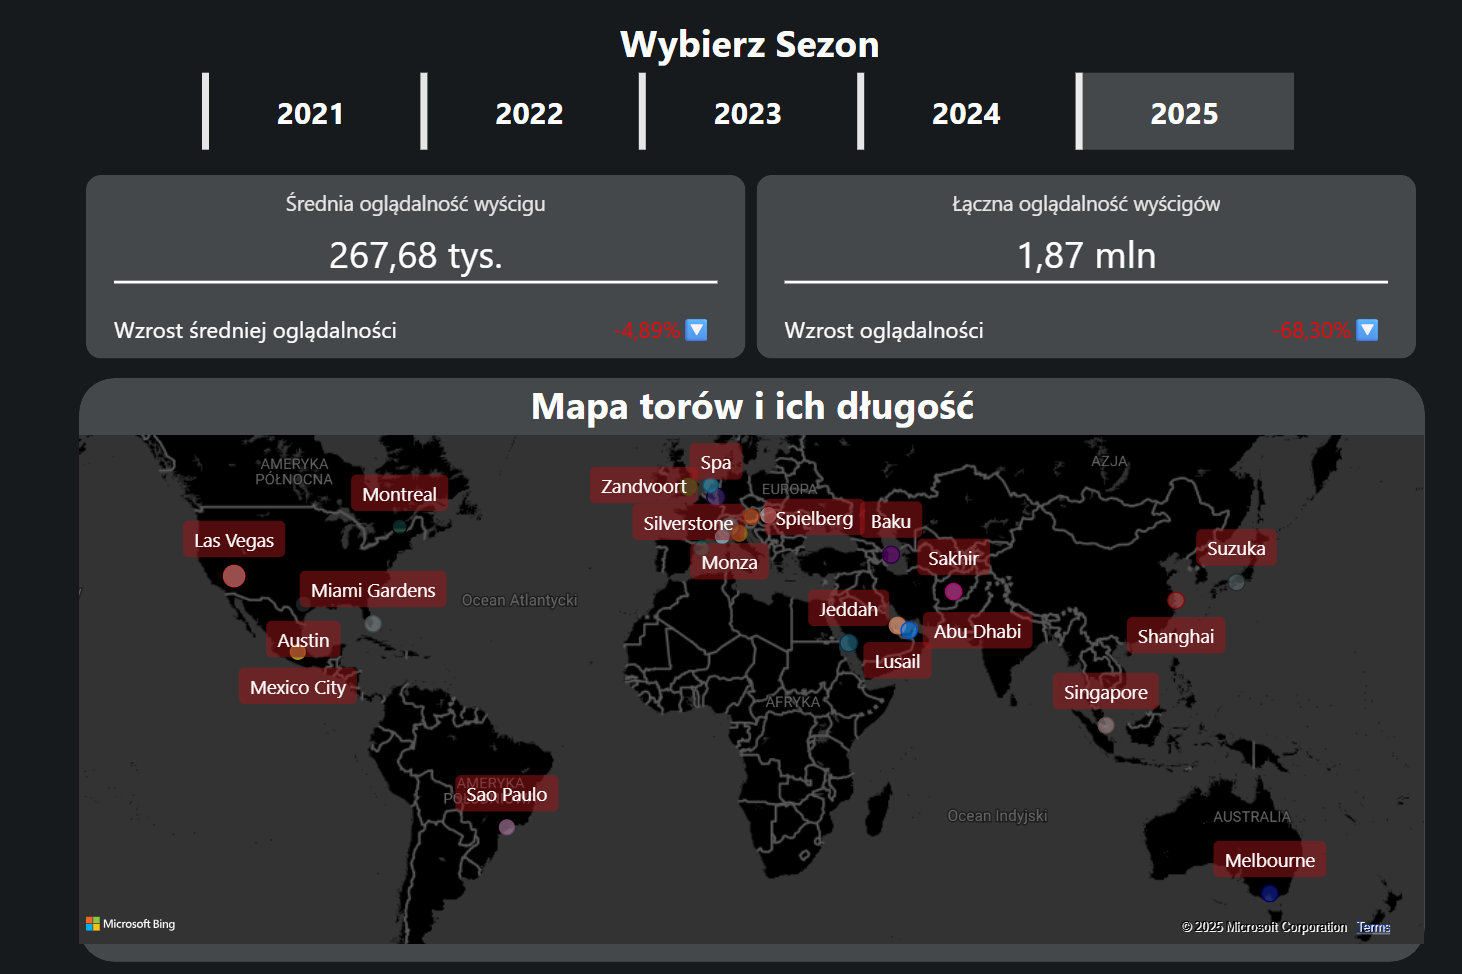
\includegraphics[width=\textwidth]{t8.png}
    \caption{Test wykresu}
\end{figure}

\begin{figure}[H]
    \centering   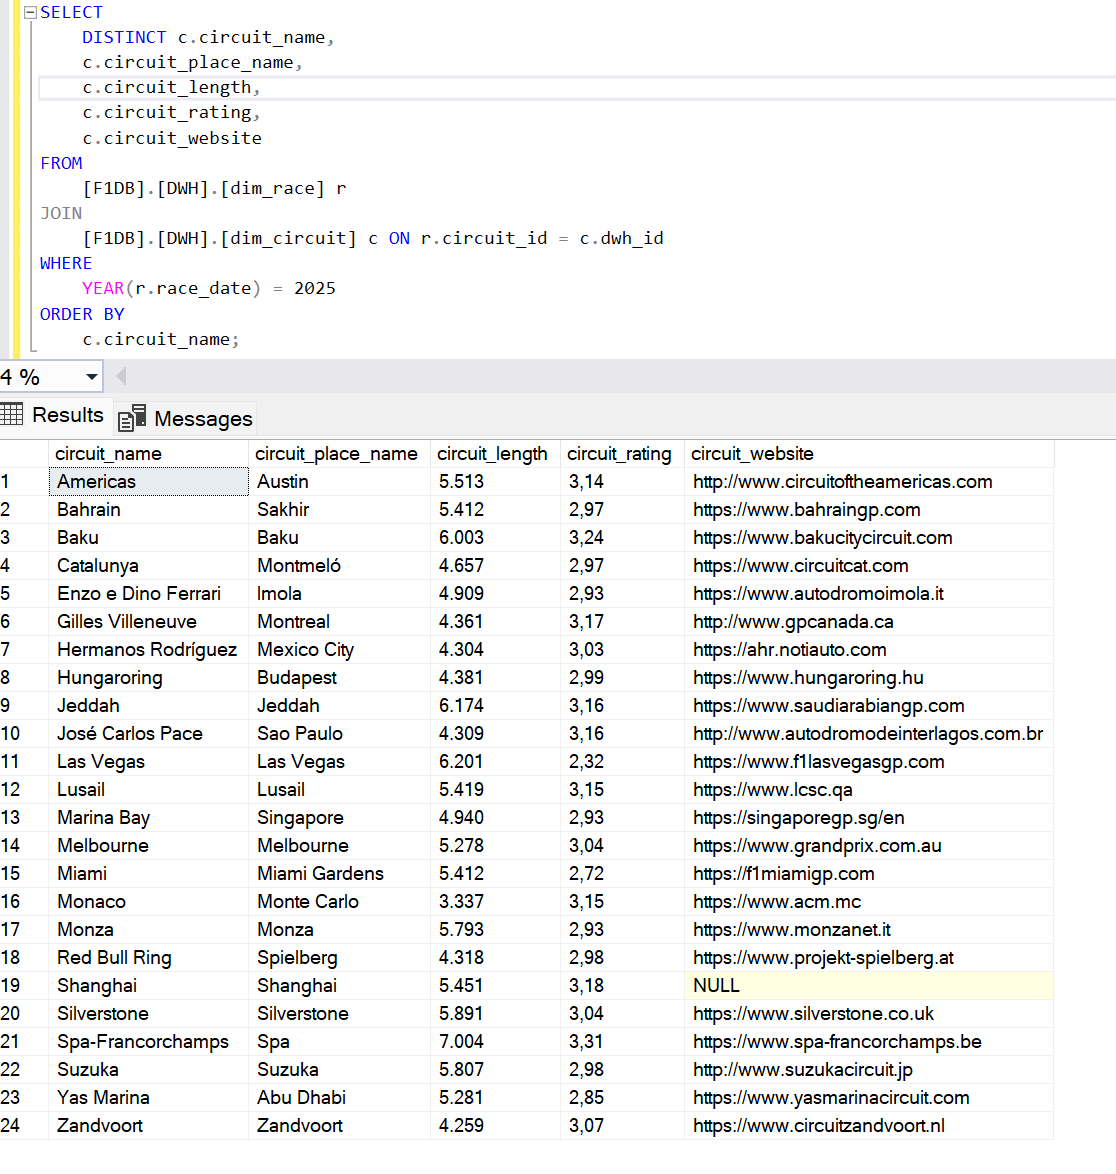
\includegraphics[width=\textwidth]{t9.png}
    \caption{Odpowiednia kwerenda}
\end{figure}

\begin{figure}[H]
    \centering   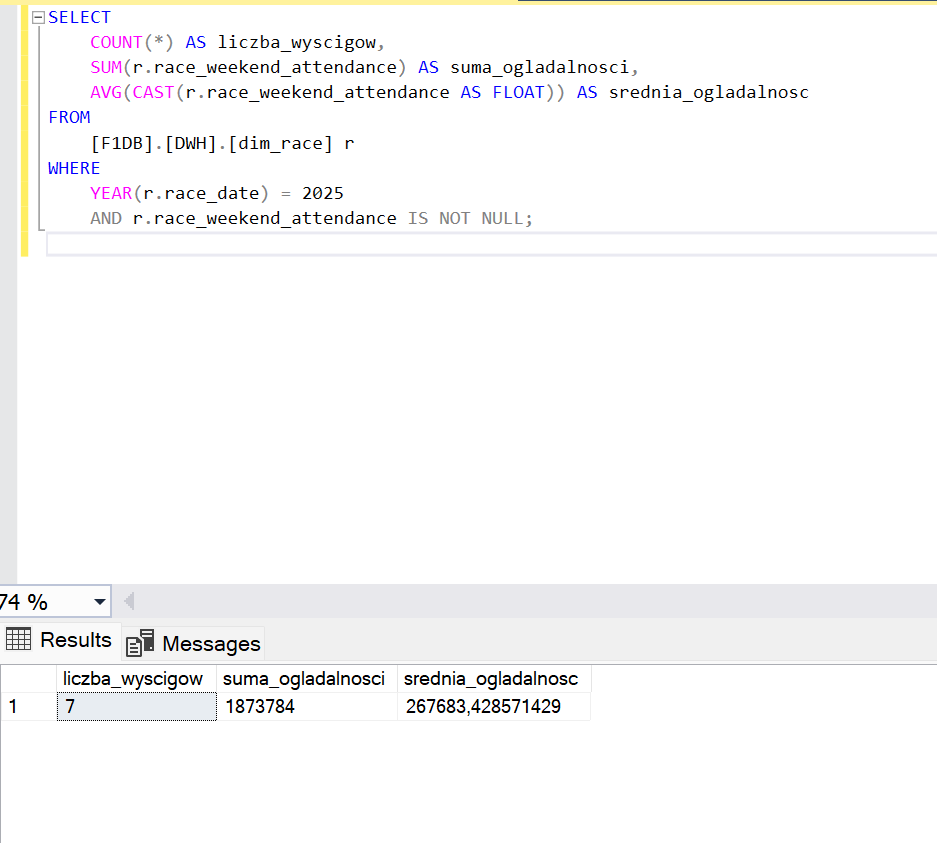
\includegraphics[width=\textwidth]{t10.png}
    \caption{Odpowiednia kwerenda}
\end{figure}

\subsubsection*{4 strona raportu}
Cel i założenia są te same co wyżej.
\begin{figure}[H]
    \centering   \includegraphics[width=\textwidth]{t11.png}
    \caption{Test wykresu}
\end{figure}

\begin{figure}[H]
    \centering   \includegraphics[width=\textwidth]{t12.png}
    \caption{Odpowiednia kwerenda}
\end{figure}

\begin{figure}[H]
    \centering   \includegraphics[width=\textwidth]{t13.png}
    \caption{Odpowiednia kwerenda}
\end{figure}

\begin{figure}[H]
    \centering   \includegraphics[width=\textwidth]{t14.png}
    \caption{Odpowiednia kwerenda}
\end{figure}

\subsubsection*{5 strona raportu}
Cel i założenia są te same co wyżej.
\begin{figure}[H]
    \centering   \includegraphics[width=\textwidth]{t15.png}
    \caption{Test wykresu}
\end{figure}

\begin{figure}[H]
    \centering   \includegraphics[width=\textwidth]{t16.png}
    \caption{Test wykresu}
\end{figure}

\end{document}
